% Chương 4: Thực nghiệm và đánh giá
\section{Giới thiệu}

Để đánh giá hiệu quả của hệ thống điều khiển đèn giao thông thông minh, nghiên
cứu này đã tiến hành một quy trình thực nghiệm toàn diện bao gồm ba thành phần
chính: (1) Phát triển và tối ưu hóa các mô hình Deep Q-Network (DQN) cho điều khiển
giao lộ đơn, (2) Phát triển hoàn toàn mới hệ thống Tác nhân Đồng bộ (Sync Agent) để giải quyết
thách thức điều phối đồng bộ nhiều giao lộ, và (3) Phân tích tác động của độ phức tạp
giao thông đến hiệu suất Học Tăng Cường Sâu (Deep Reinforcement Learning).

Nghiên cứu tập trung đặc biệt vào việc phân tích ảnh hưởng của mức độ giao thông khác nhau
đến khả năng hội tụ (convergence) và hiệu suất cuối cùng của mô hình DQN. Điều này bao gồm việc đánh giá
hiệu suất trên 4 kịch bản giao thông từ thấp đến cao điểm (300-1200 xe/giờ), cung cấp
những hiểu biết thực tế về khả năng triển khai (deployment) trong các điều kiện giao thông khác nhau.

Đặc biệt, nghiên cứu đã thành công trong việc phát triển Tác nhân Đồng bộ (Sync Agent) - một thành phần hoàn toàn
mới được thiết kế từ đầu để giải quyết bài toán đồng bộ hóa tín hiệu giao thông
đa giao lộ, đồng thời vượt qua các thách thức kỹ thuật về tính ổn định huấn luyện.

\section{Tiêu chí đánh giá}

\subsection{Các chỉ số hiệu suất chính}
Nghiên cứu sử dụng các tiêu chí đánh giá sau để đo lường hiệu quả của hệ thống:

\subsubsection{Thời gian chờ đợi trung bình (Average Waiting Time)}
\begin{itemize}
    \item \textbf{Định nghĩa:} Thời gian trung bình mà các phương tiện phải chờ tại giao lộ
    \item \textbf{Đơn vị:} Giây (s)
    \item \textbf{Ý nghĩa:} Thấp hơn = hiệu suất tốt hơn
    \item \textbf{Công thức:} $\bar{W} = \frac{1}{N} \sum_{i=1}^{N} W_i$ với $W_i$ là thời gian chờ của xe $i$
\end{itemize}

\subsubsection{Độ dài hàng đợi trung bình (Average Queue Length)}
\begin{itemize}
    \item \textbf{Định nghĩa:} Số lượng phương tiện trung bình trong hàng đợi tại mỗi thời điểm
    \item \textbf{Đơn vị:} Số xe
    \item \textbf{Ý nghĩa:} Thấp hơn = lưu thông tốt hơn
    \item \textbf{Công thức:} $\bar{Q} = \frac{1}{T} \sum_{t=1}^{T} Q_t$ với $Q_t$ là số xe trong hàng đợi tại thời điểm $t$
\end{itemize}

\subsubsection{Phần thưởng tích lũy (Cumulative Reward)}
\begin{itemize}
    \item \textbf{Định nghĩa:} Tổng phần thưởng nhận được trong quá trình huấn luyện
    \item \textbf{Đơn vị:} Điểm số
    \item \textbf{Ý nghĩa:} Cao hơn = mô hình học tốt hơn
    \item \textbf{Mục tiêu:} Tối đa hóa giá trị này thông qua quá trình huấn luyện
\end{itemize}

\subsection{Tiêu chí thành công}
\begin{itemize}
    \item \textbf{Cải thiện tối thiểu:} ≥10\% so với hệ thống cố định (fixed-time)
    \item \textbf{Độ ổn định:} Phương sai thời gian chờ ≤15\% giá trị trung bình
    \item \textbf{Hội tụ huấn luyện:} Đạt được trong vòng 150 episodes
    \item \textbf{Ý nghĩa thống kê:} p-value < 0.05 cho các so sánh hiệu suất
\end{itemize}

\section{Thiết lập thí nghiệm}

\subsection{Môi trường mô phỏng cho giao lộ đơn}
Các thực nghiệm được tiến hành trên một giao lộ 4 chiều với các thông số sau:
\begin{itemize}
    \item Số làn xe mỗi hướng: 2 làn

    \item Chiều dài đoạn đường mỗi hướng: 150m

    \item Tốc độ tối đa cho phép: 50 km/h

    \item Thời gian mô phỏng: 3600 giây (1 giờ)

    \item Số tập huấn luyện (episode): 150-300 tập tùy theo mô hình
\end{itemize}

\subsection{Môi trường mô phỏng cho hệ thống đồng bộ}
Để đánh giá Tác nhân Đồng bộ (Sync Agent), nghiên cứu sử dụng:
\begin{itemize}
    \item Mạng lưới 3 giao lộ kết nối tuyến tính

    \item Khoảng cách giữa các giao lộ: 200-500m

    \item Tốc độ giao thông đô thị: 25-45 km/h

    \item Các kịch bản lưu lượng giao thông: thấp (30), bình thường (45), cao (70), giờ cao
        điểm (90)

    \item Số tập huấn luyện: 150 tập cho mỗi cấu hình phần thưởng
\end{itemize}

\subsection{Cấu hình các mô hình giao lộ đơn}

Để đảm bảo tính khách quan và độ tin cậy trong việc so sánh, nghiên cứu đã thiết
lập mười cấu hình khác nhau với các tham số huấn luyện đa dạng. Mỗi cấu hình
được thiết kế để kiểm tra ảnh hưởng của các yếu tố cụ thể như tốc độ học, kích thước
lô, kiến trúc mạng và các tham số môi trường.

Các cấu hình được thiết kế với mục đích cụ thể như sau:
\begin{itemize}
    \item \textbf{Original:} Cấu hình đầu tiên được xây dựng
    
    \item \textbf{Baseline:} Sử dụng các tham số được khuyến nghị trong 
        các nghiên cứu DQN cơ bản làm điểm tham chiếu (tốc độ học = 0.0005, kích thước lô = 64, 
        gamma = 0.75) 

    \item \textbf{Conservative:} Tốc độ học thấp, nhằm đảm bảo sự ổn định

    \item \textbf{High Traffic:} Tối ưu cho điều kiện giao thông
        cao điểm

    \item \textbf{Low Traffic:} Tối ưu cho điều kiện giao thông
        thấp điểm

    \item \textbf{Balanced:} Cân bằng giữa tốc độ học và độ ổn định

    \item \textbf{Medium Batch:} Kiểm tra ảnh hưởng của kích
        thước lô

    \item \textbf{Moderate Learning:} Tốc độ học trung bình


    \item \textbf{Aggressive:} Tham số mạnh mẽ để tăng tốc quá trình
        học

    \item \textbf{High Learning:} Tốc độ học rất cao để kiểm tra giới
        hạn ổn định
\end{itemize}

\section{Kết quả và phân tích hiệu suất giao lộ đơn}

Sau quá trình huấn luyện và đánh giá trong môi trường mô phỏng SUMO, các mô hình
được đánh giá dựa trên ba tiêu chí chính: giá trị phần thưởng (reward) tích lũy, thời
gian chờ đợi trung bình và độ dài hàng đợi trung bình.

\subsection{Trực quan hóa kết quả huấn luyện}

Để phân tích hiệu suất một cách trực quan và khách quan, nghiên cứu trình bày
kết quả dưới dạng biểu đồ. Do hai mô hình Aggressive và High Learning có hiệu suất
cực kỳ kém (với giá trị phần thưởng âm rất lớn), việc đưa chúng vào cùng biểu đồ
sẽ làm biến dạng dạng thang đo và khó quan sát sự khác biệt giữa các mô hình có hiệu
suất hợp lý khác. Vì vậy, kết quả được trình bày trong hai biểu đồ riêng biệt, hai mô hình có hiệu suất kém được hiển thị trong phần so sánh với giá trị ngoại lai (outliers).

\subsubsection{Tiến trình phần thưởng qua các tập huấn luyện}

\begin{figure}[!htp]
    \centering
    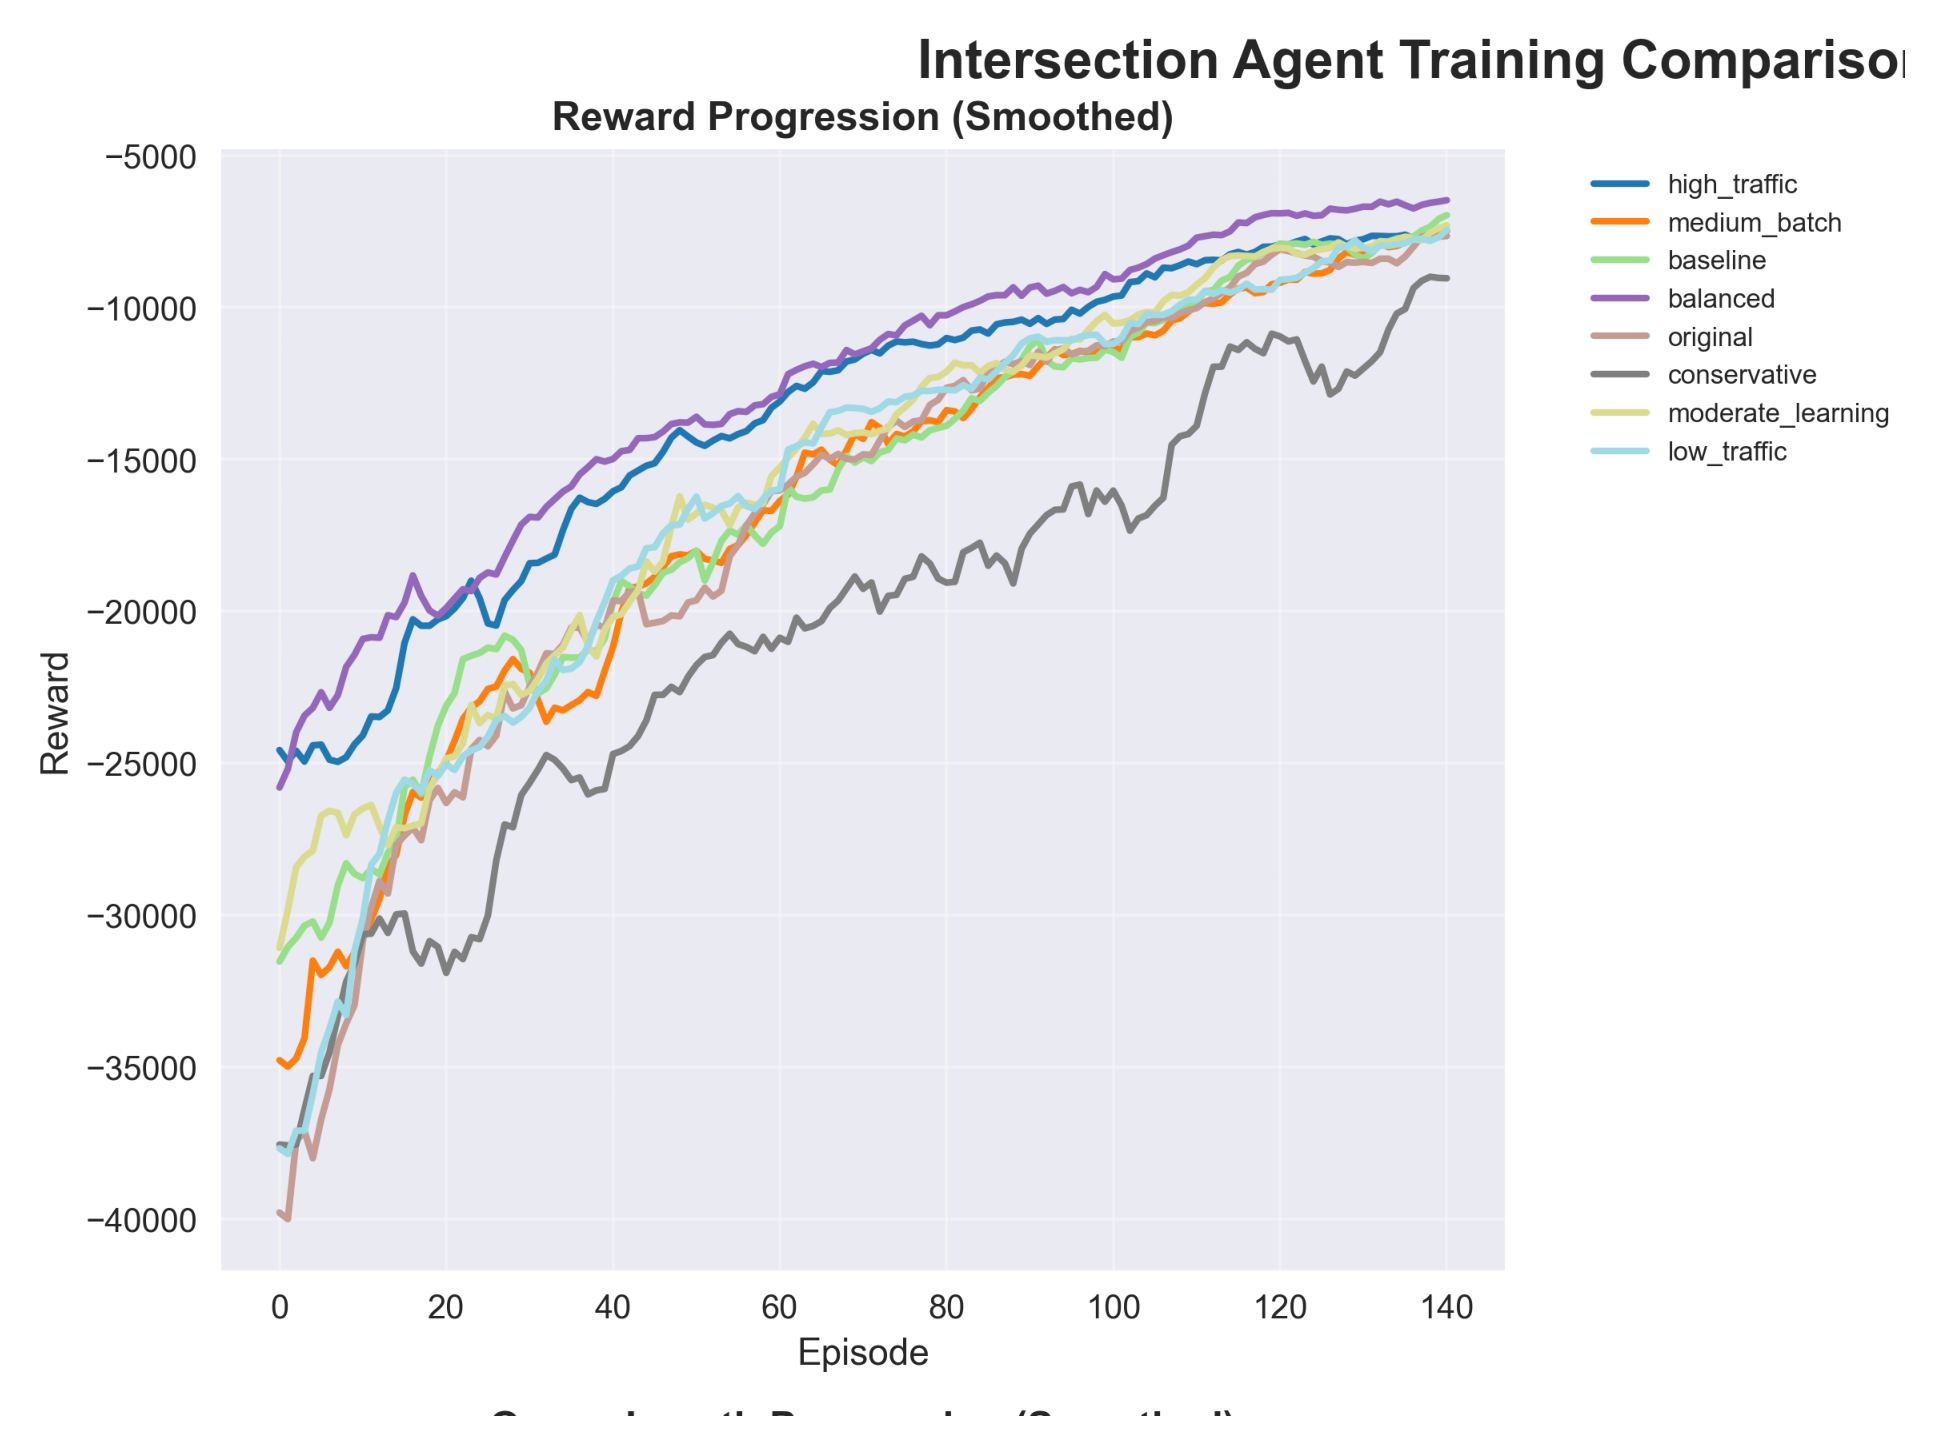
\includegraphics[width=\textwidth]{
        figures/individual_plots/intersection_filtered_reward_progress.png
    }
    \caption{Tiến trình phần thưởng của các mô hình intersection agent qua các
    tập huấn luyện (loại bỏ giá trị ngoại lai)}
    \label{fig:intersection_filtered_reward_progress}
\end{figure}

Hình \ref{fig:intersection_filtered_reward_progress} thể hiện quá trình học của
8 mô hình có hiệu suất khả thi. Mô hình Balanced cho thấy sự hội tụ ổn định nhất
với phần thưởng cuối cùng đạt -12,860, trong khi các mô hình khác có độ biến động lớn
hơn.

\subsubsection{Thời gian chờ đợi trung bình}

\begin{figure}[!htp]
    \centering
    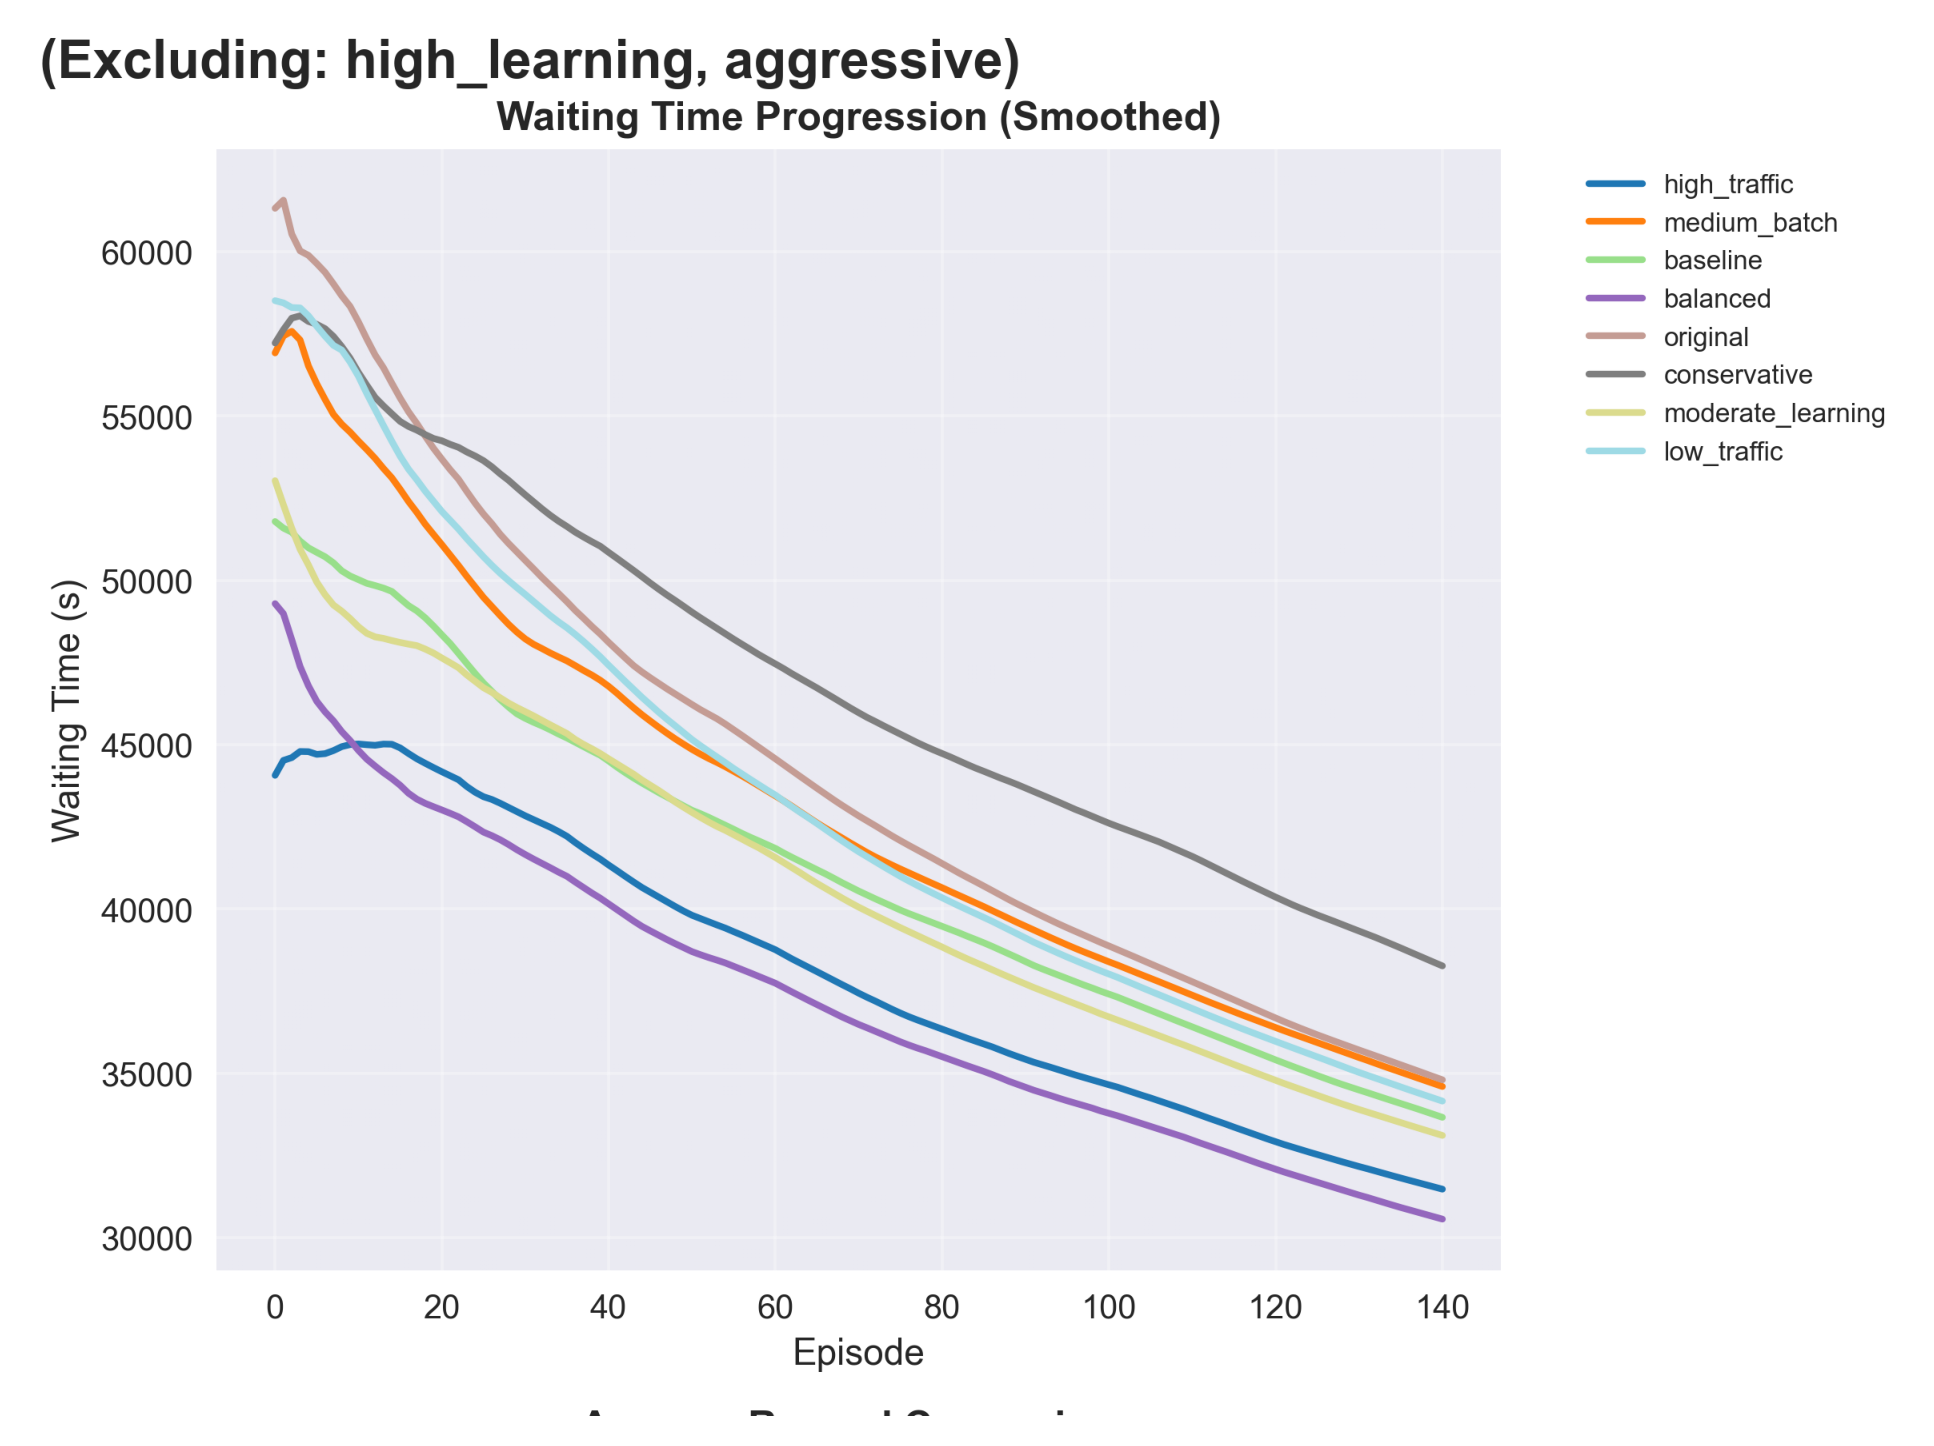
\includegraphics[width=\textwidth]{
        figures/individual_plots/intersection_filtered_waiting_time.png
    }
    \caption{So sánh thời gian chờ đợi trung bình của các mô hình intersection
    agent}
    \label{fig:intersection_filtered_waiting_time}
\end{figure}

Hình \ref{fig:intersection_filtered_waiting_time} cho thấy mô hình Balanced đạt thời
gian chờ thấp nhất (37,506s), vượt trội so với các mô hình khác. Điều này chứng minh
hiệu quả của việc cân bằng các siêu tham số (hyperparameter).

\subsubsection{Độ dài hàng đợi trung bình}

\begin{figure}[!htp]
    \centering
    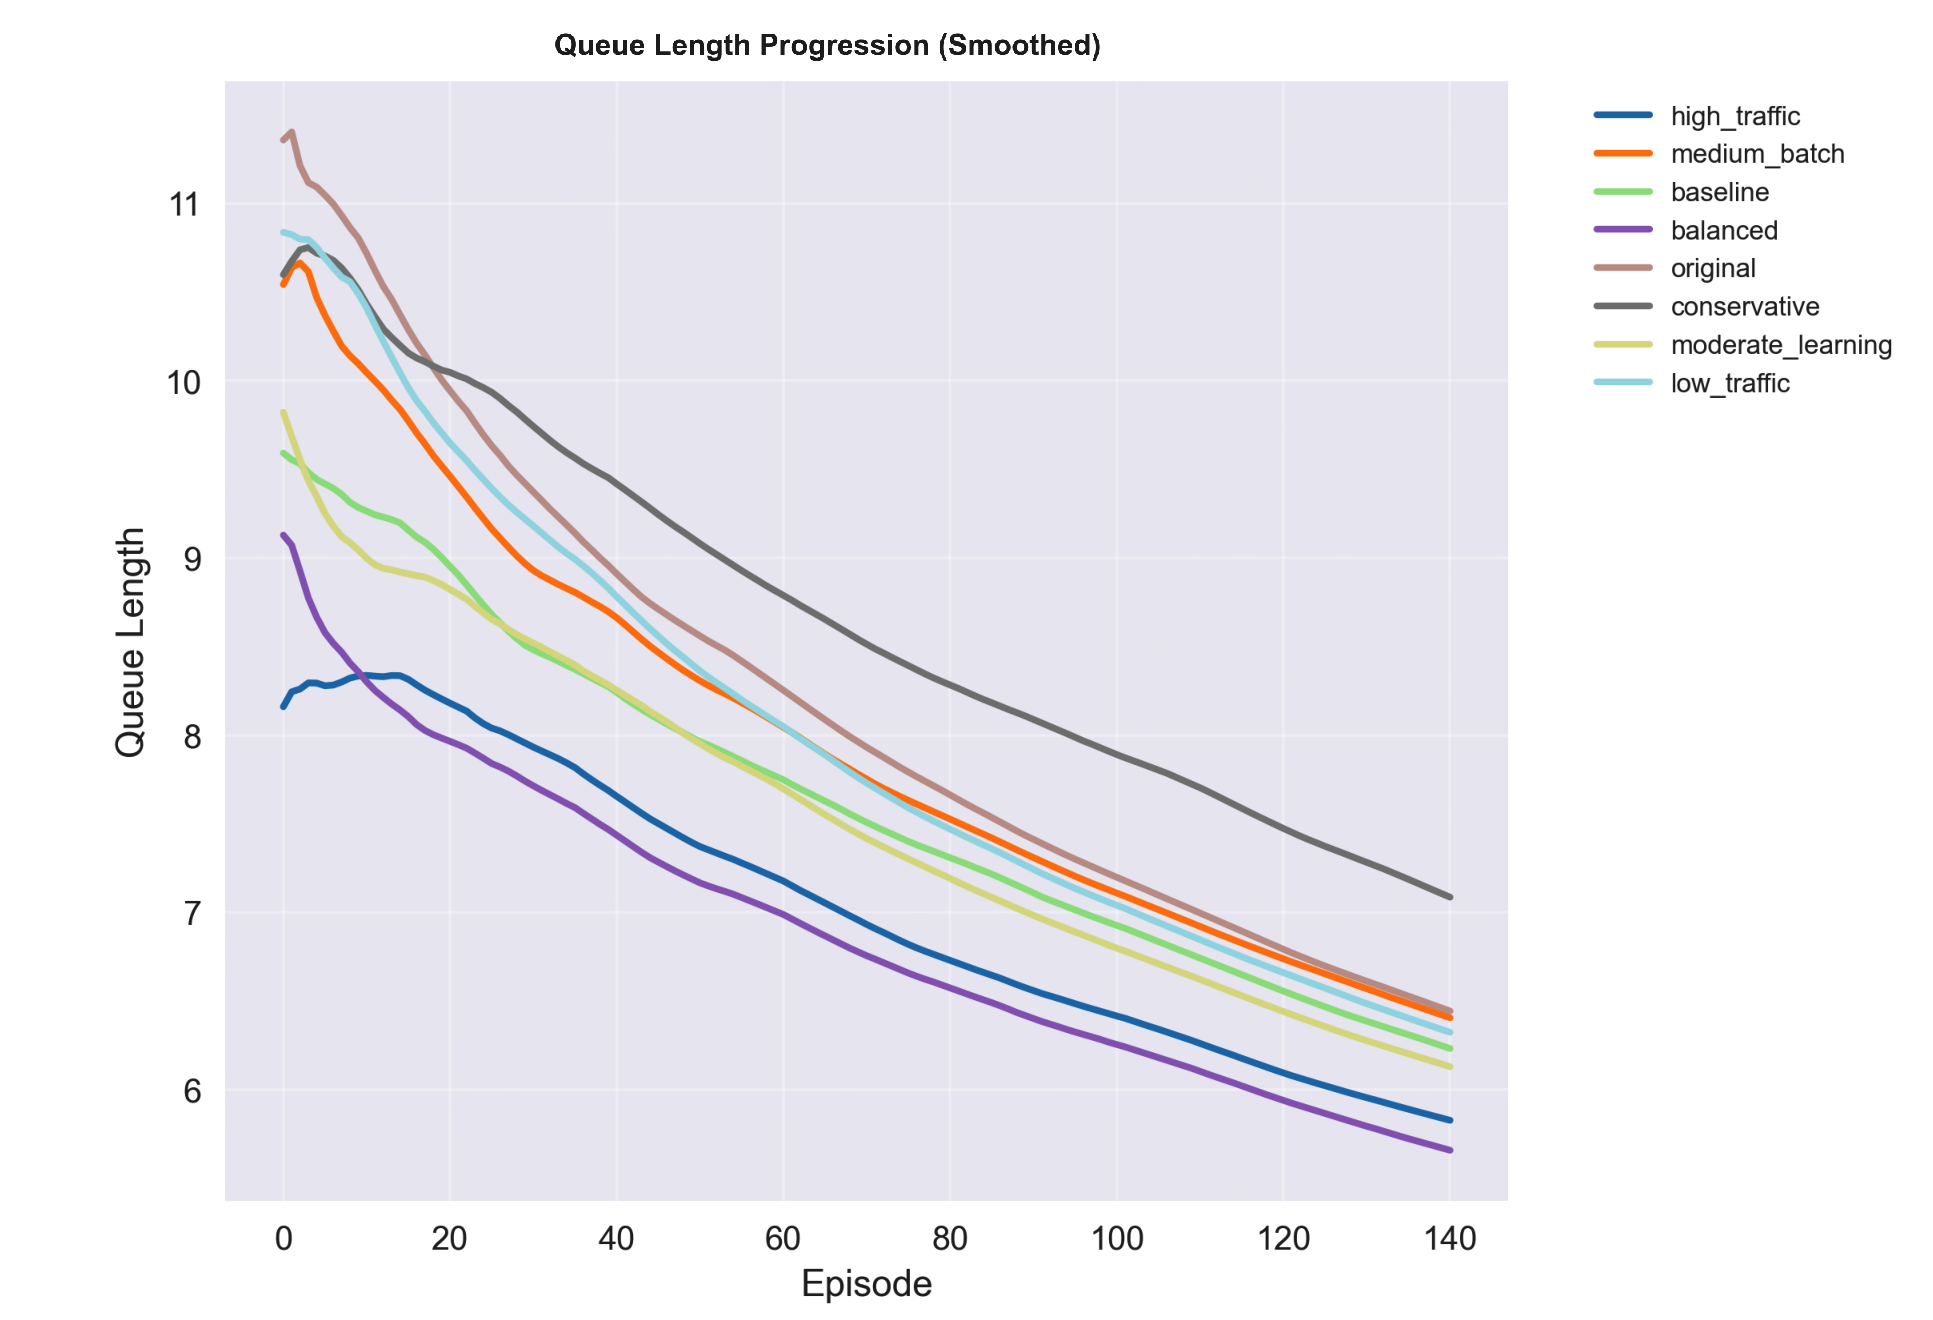
\includegraphics[width=\textwidth]{
        figures/individual_plots/intersection_filtered_queue_length.png
    }
    \caption{So sánh độ dài hàng đợi trung bình của các mô hình intersection
    agent}
    \label{fig:intersection_filtered_queue_length}
\end{figure}

Hình \ref{fig:intersection_filtered_queue_length} thể hiện mô hình Balanced cũng
đạt độ dài hàng đợi nhỏ nhất (6.95 xe), tương quan trực tiếp với hiệu suất thời
gian chờ đợi.

\subsubsection{So sánh tổng thể hiệu suất}

\begin{figure}[!htp]
    \centering
    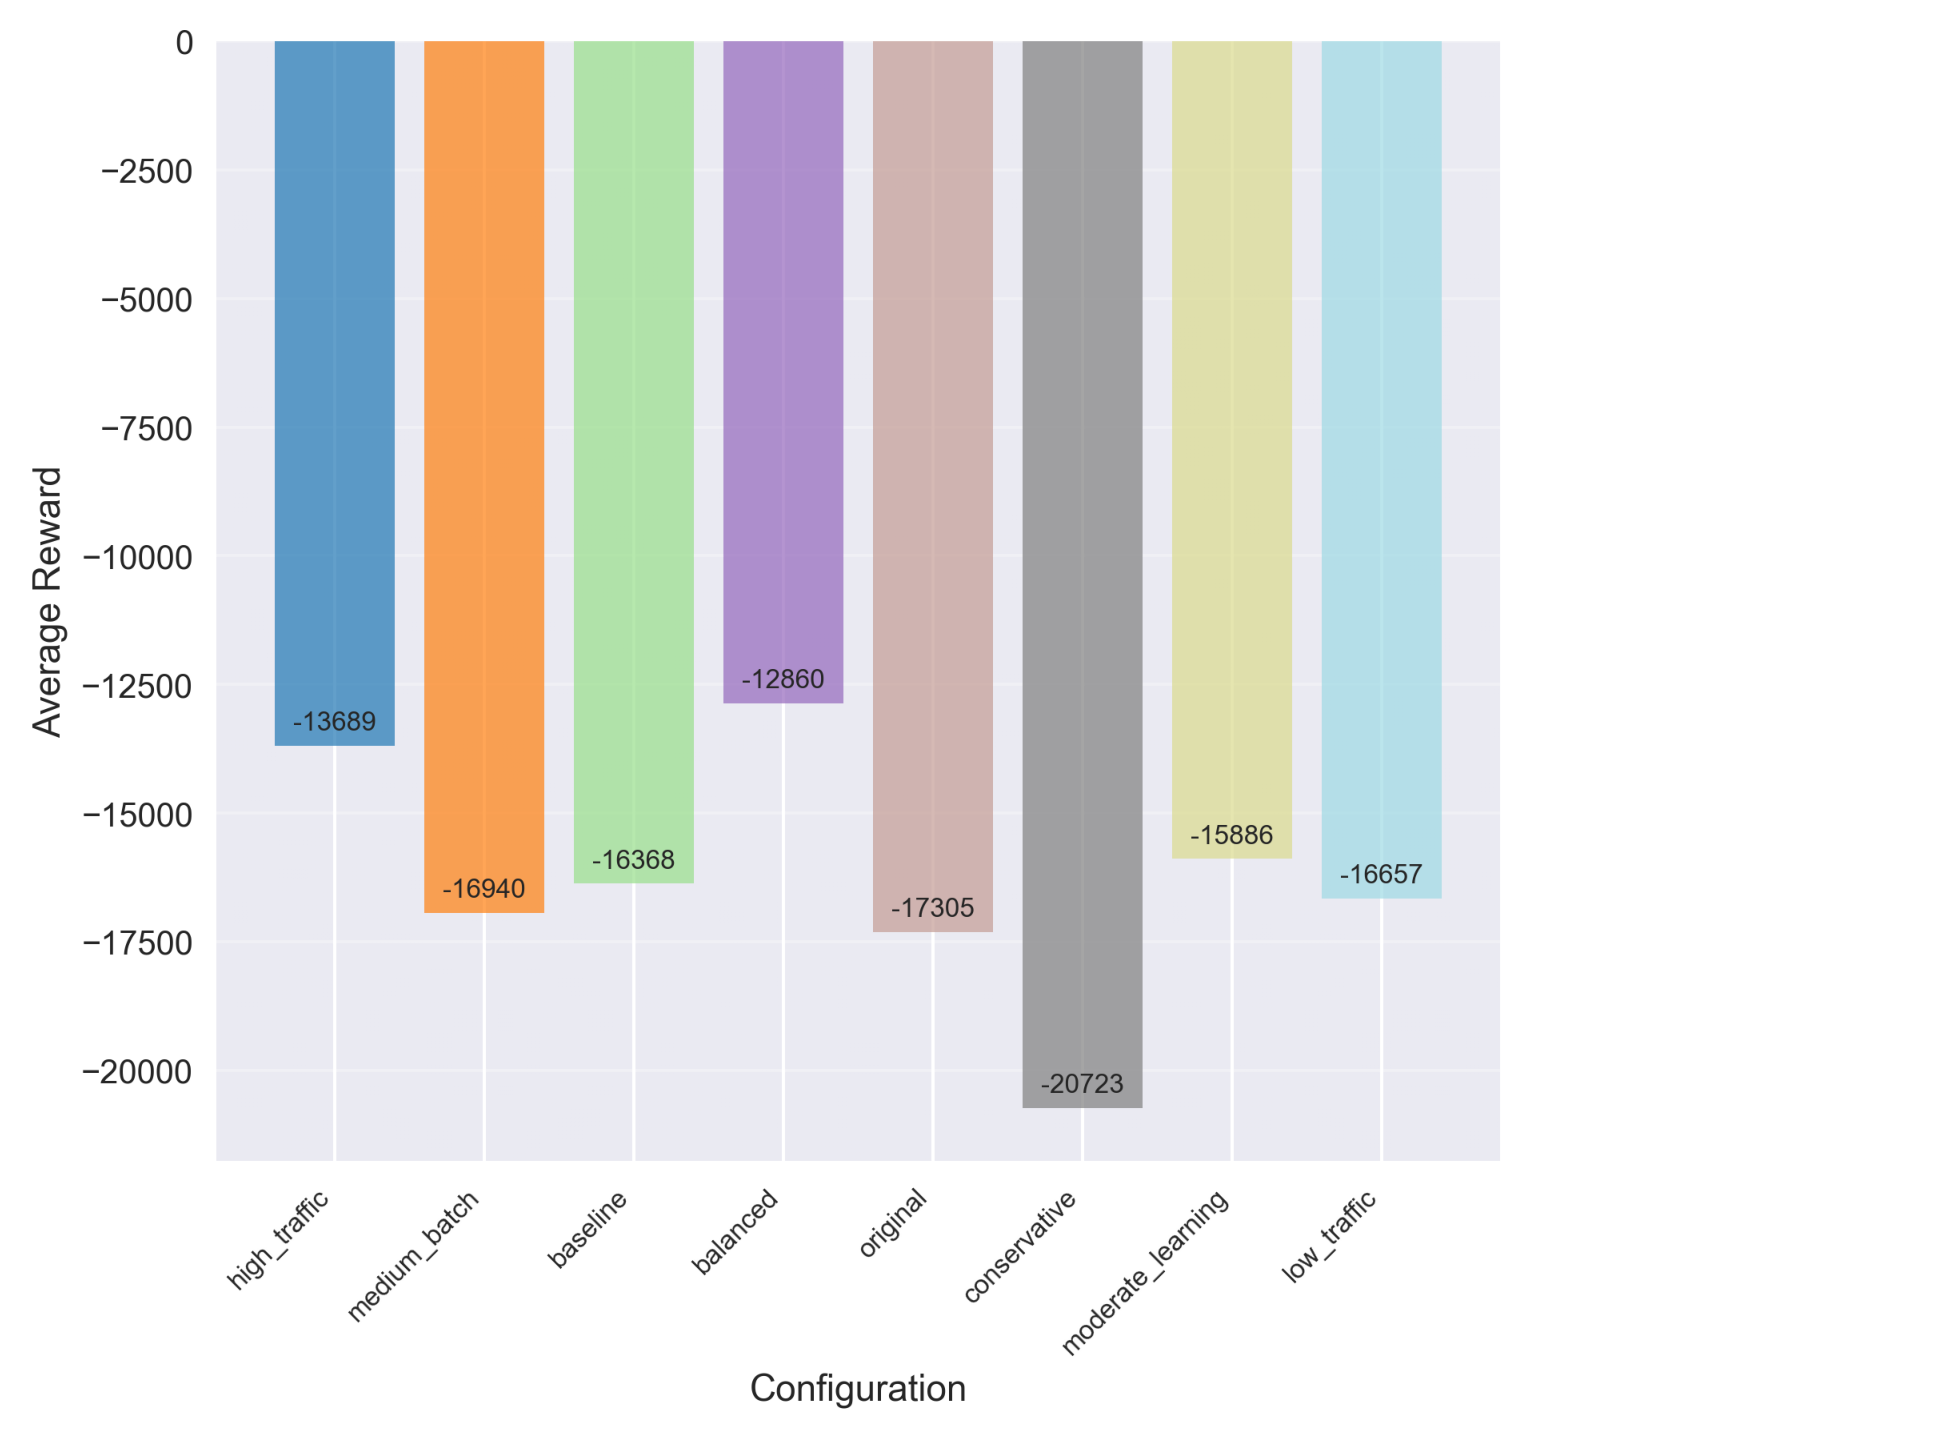
\includegraphics[width=\textwidth]{
        figures/individual_plots/intersection_filtered_performance_summary.png
    }
    \caption{Tổng hợp so sánh hiệu suất các mô hình intersection agent}
    \label{fig:intersection_filtered_performance_summary}
\end{figure}

Hình \ref{fig:intersection_filtered_performance_summary} tổng hợp các chỉ số
hiệu suất, khẳng định sự vượt trội của mô hình Balanced trong tất cả các tiêu chí
đánh giá.

\subsection{So sánh đầy đủ bao gồm giá trị ngoại lai}

Để thể hiện tác động nghiêm trọng của việc lựa chọn siêu tham số không phù hợp,
nghiên cứu cũng trình bày kết quả đầy đủ của tất cả 10 mô hình bao gồm cả hai mô
hình có hiệu suất cực kém.

\subsubsection{Tiến trình reward với giá trị ngoại lai}

\begin{figure}[!htp]
    \centering
    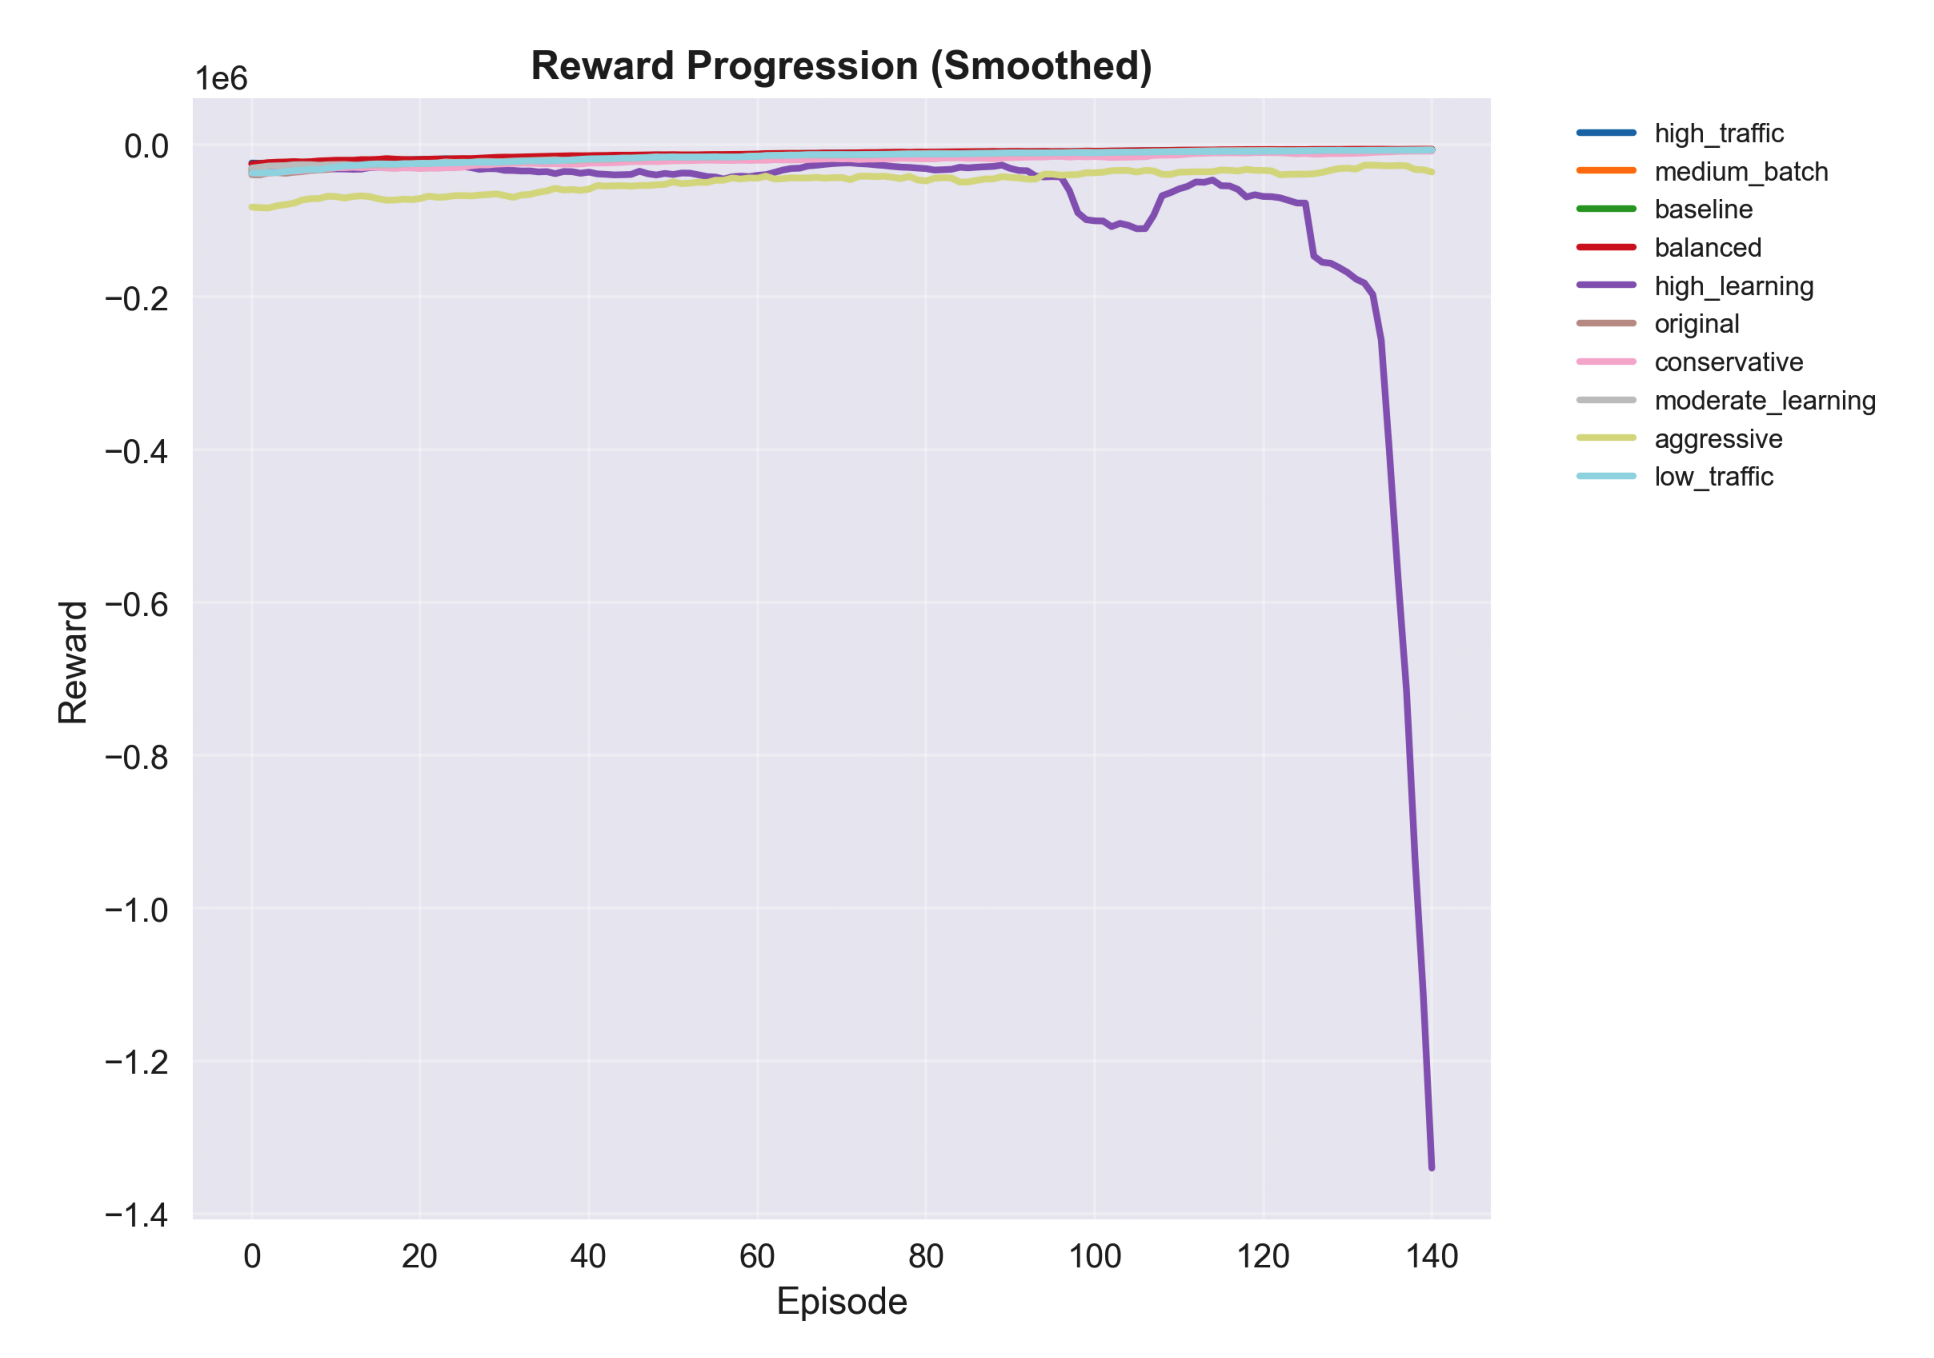
\includegraphics[width=\textwidth]{
        figures/individual_plots/intersection_full_reward_progress.png
    }
    \caption{Tiến trình phần thưởng của tất cả 10 mô hình intersection agent bao gồm giá trị ngoại lai}
    \label{fig:intersection_full_reward_progress}
\end{figure}

Hình \ref{fig:intersection_full_reward_progress} cho thấy rõ ràng sự khác biệt lớn
giữa các mô hình. Mô hình High Learning có hiệu suất cực kỳ kém với phần thưởng đạt -138,191,
trong khi Aggressive cũng thất bại với -50,135.

\subsubsection{Thời gian chờ đợi với giá trị ngoại lai}

\begin{figure}[!htp]
    \centering
    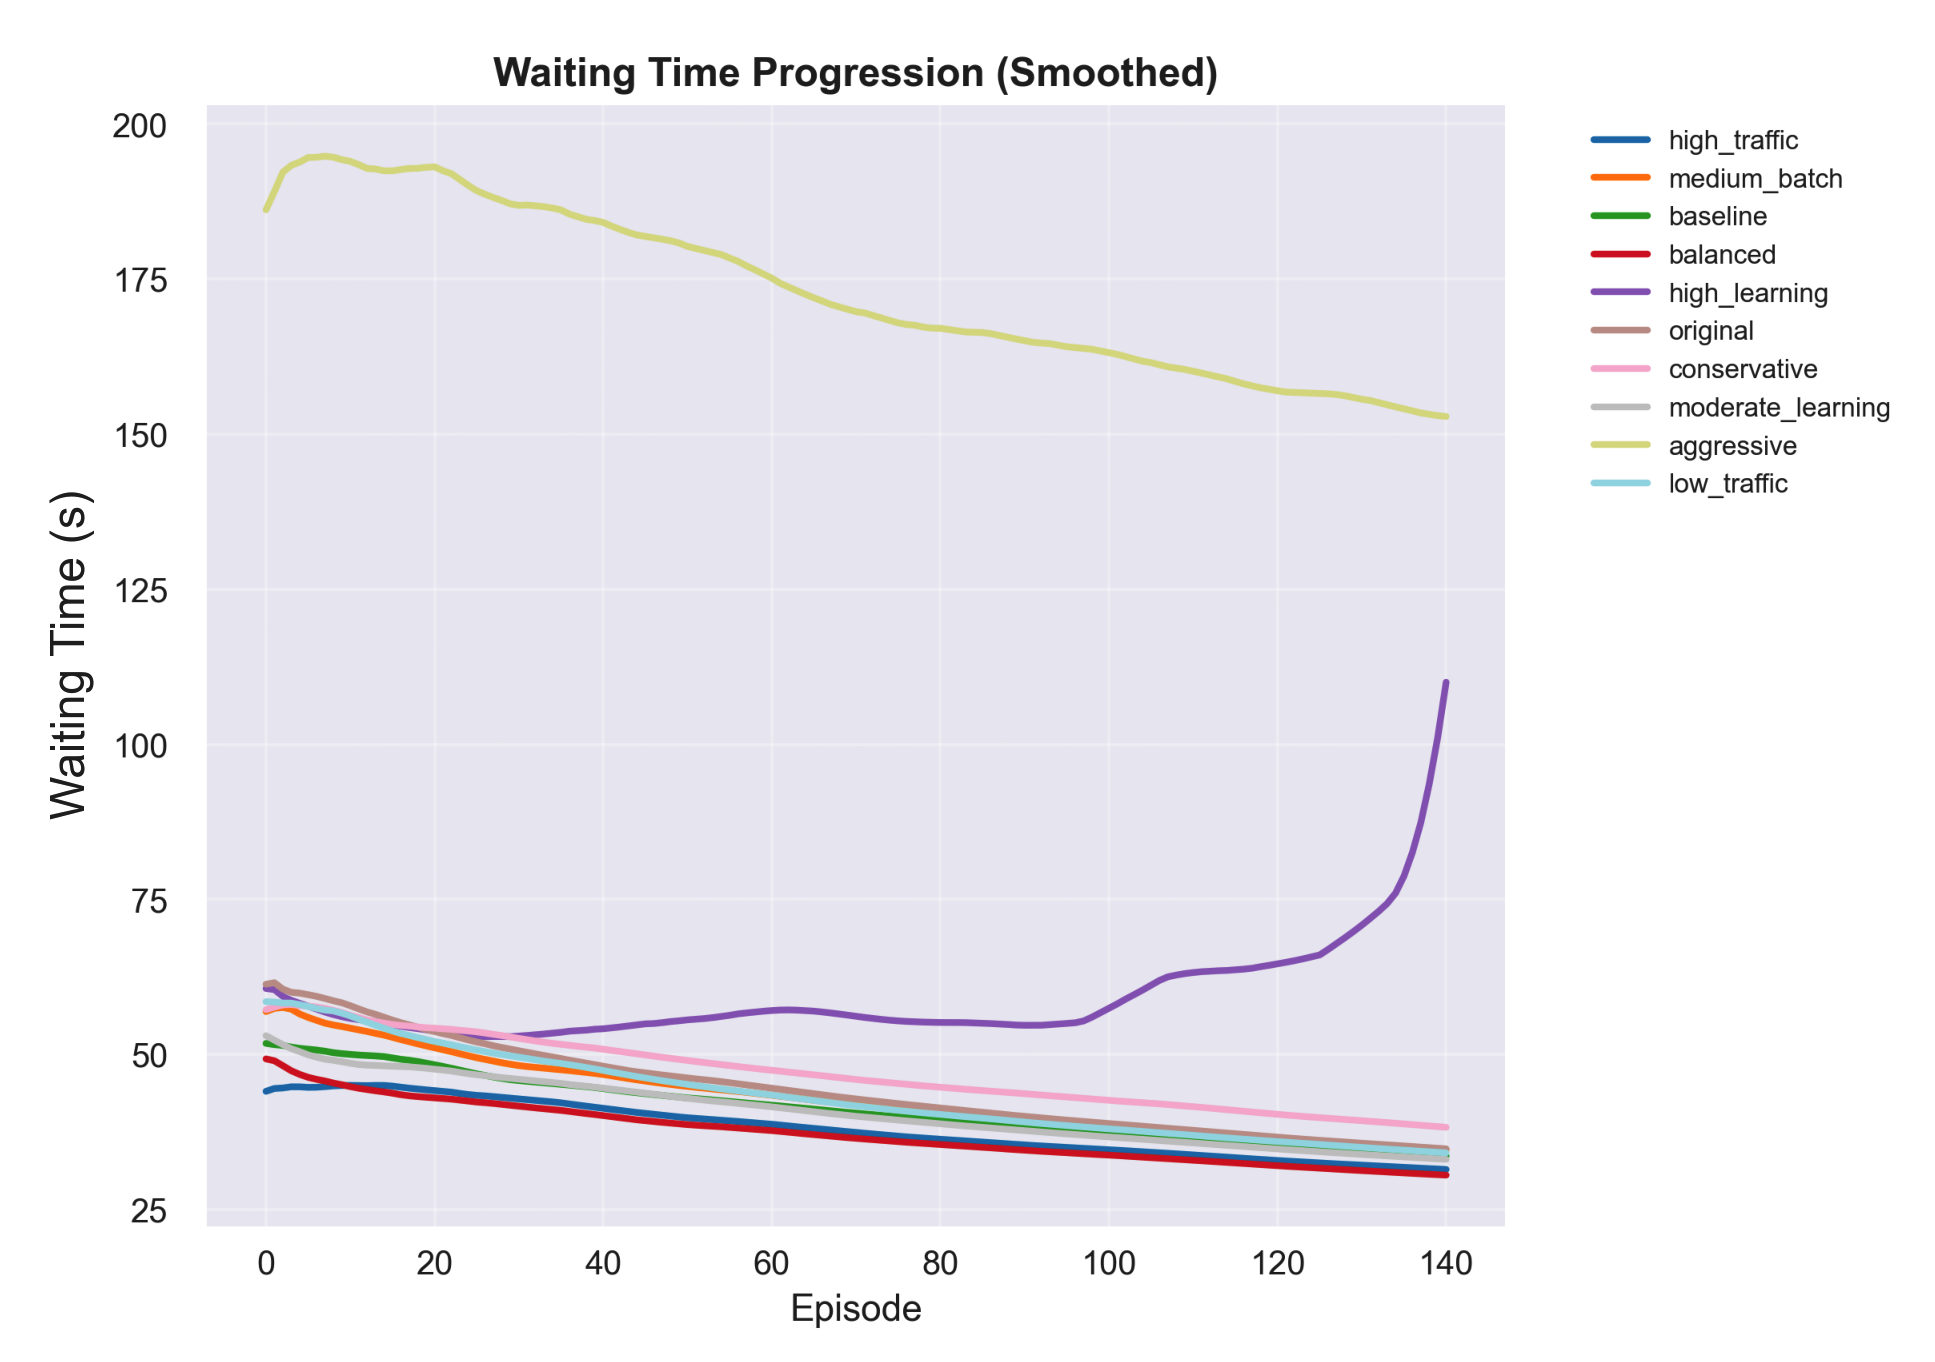
\includegraphics[width=\textwidth]{
        figures/individual_plots/intersection_full_waiting_time.png
    }
    \caption{So sánh thời gian chờ đợi của tất cả 10 mô hình bao gồm giá trị ngoại lai}
    \label{fig:intersection_full_waiting_time}
\end{figure}

Hình \ref{fig:intersection_full_waiting_time} thể hiện tác động trực tiếp của
siêu tham số không phù hợp lên hiệu suất thực tế. Mô hình Aggressive gây ra thời
gian chờ cực lớn (172,687s), gấp 4.6 lần so với mô hình Balanced.

\subsubsection{Độ dài hàng đợi với giá trị ngoại lai}

\begin{figure}[!htp]
    \centering
    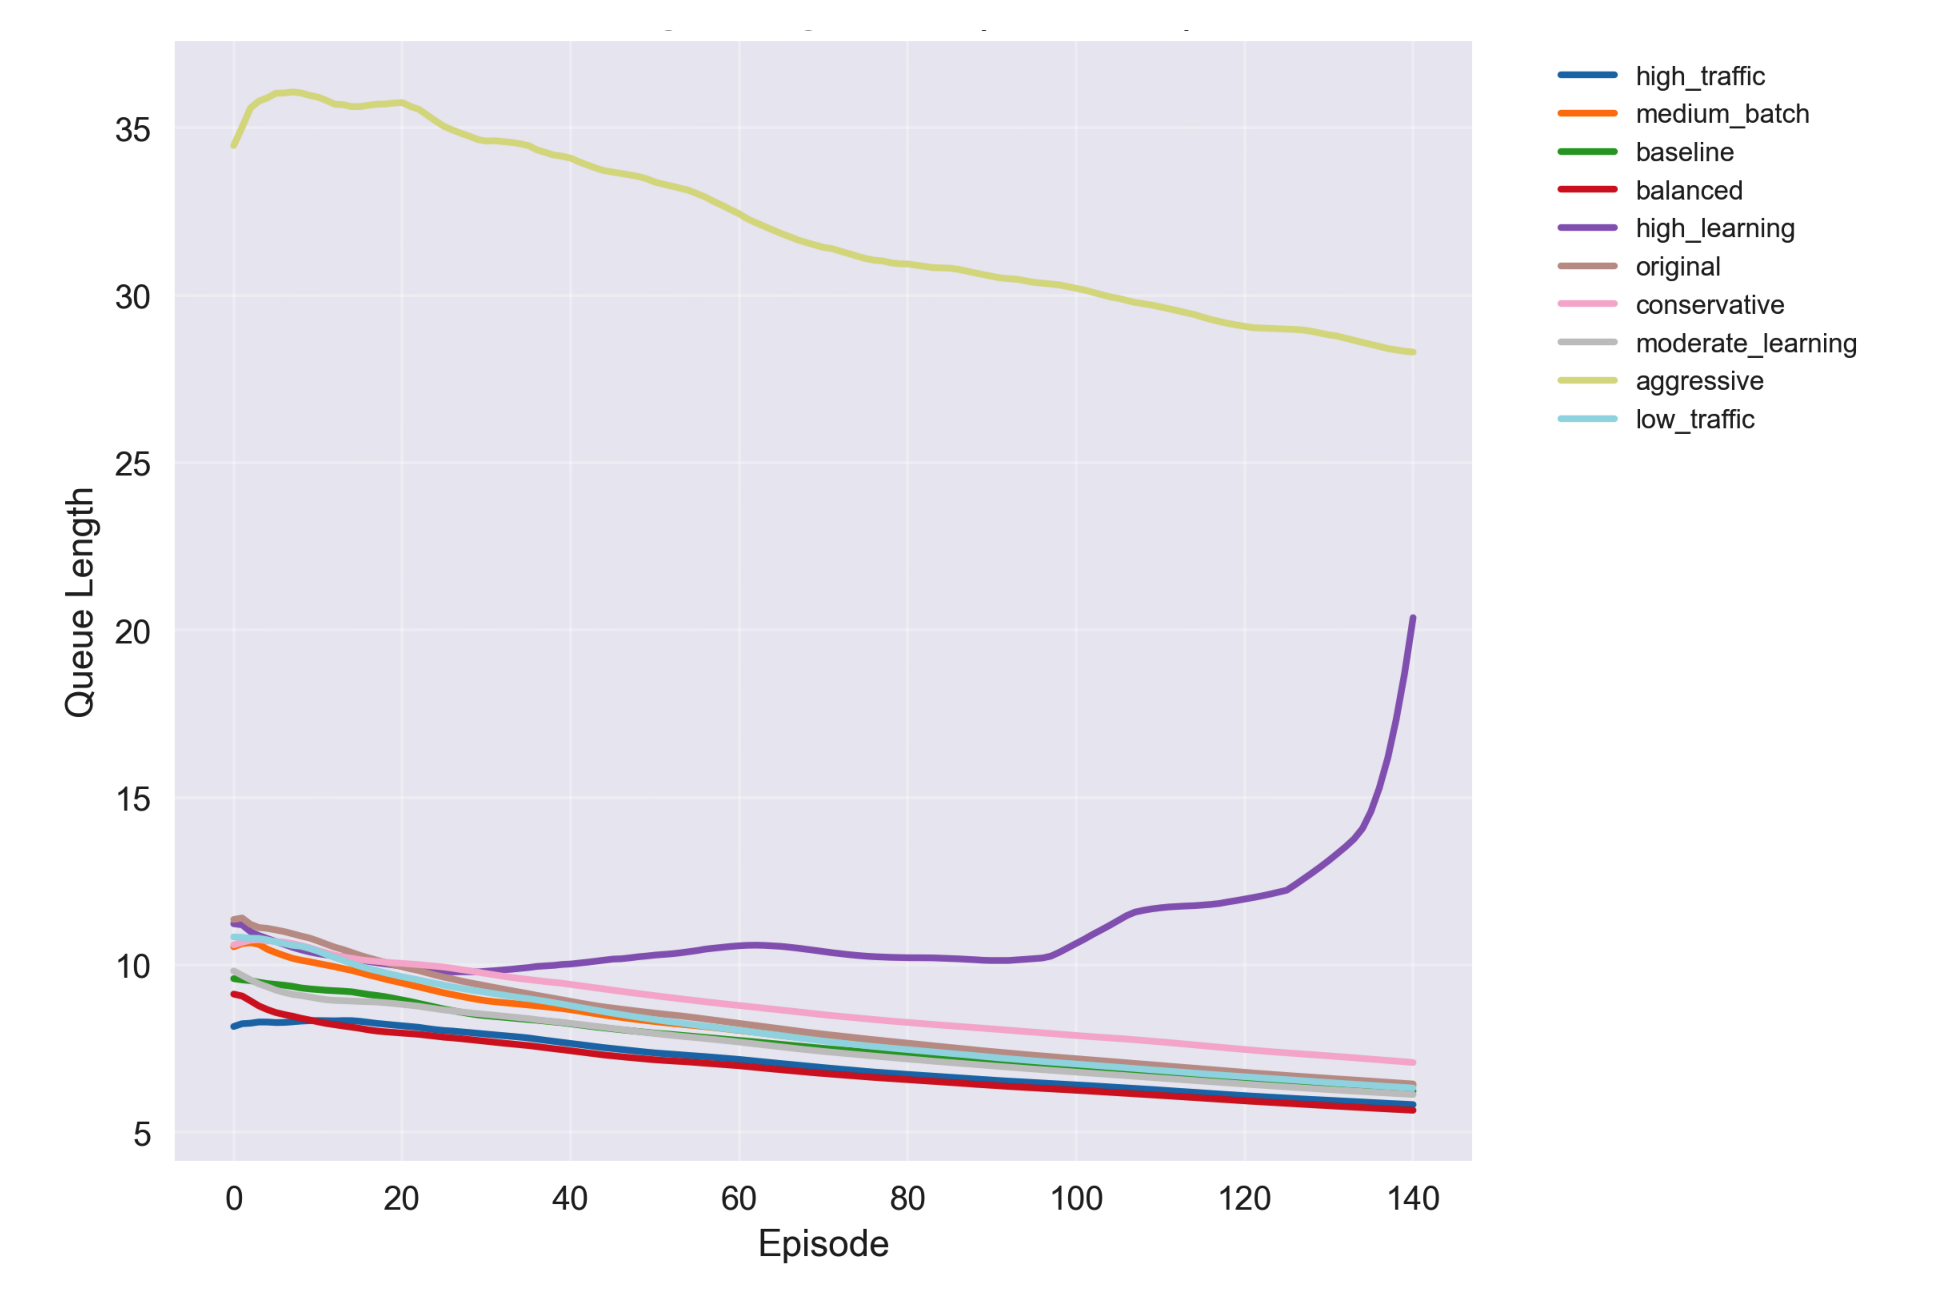
\includegraphics[width=\textwidth]{
        figures/individual_plots/intersection_full_queue_length.png
    }
    \caption{So sánh độ dài hàng đợi của tất cả 10 mô hình bao gồm giá trị ngoại lai}
    \label{fig:intersection_full_queue_length}
\end{figure}

Hình \ref{fig:intersection_full_queue_length} cho thấy mô hình Aggressive tạo ra
hàng đợi dài nhất (31.98 xe), gấp 4.6 lần so với Balanced, chứng minh tác động
nghiêm trọng của việc lựa chọn tham số không phù hợp.

\subsubsection{Tổng hợp so sánh với giá trị ngoại lai}

\begin{figure}[!htp]
    \centering
    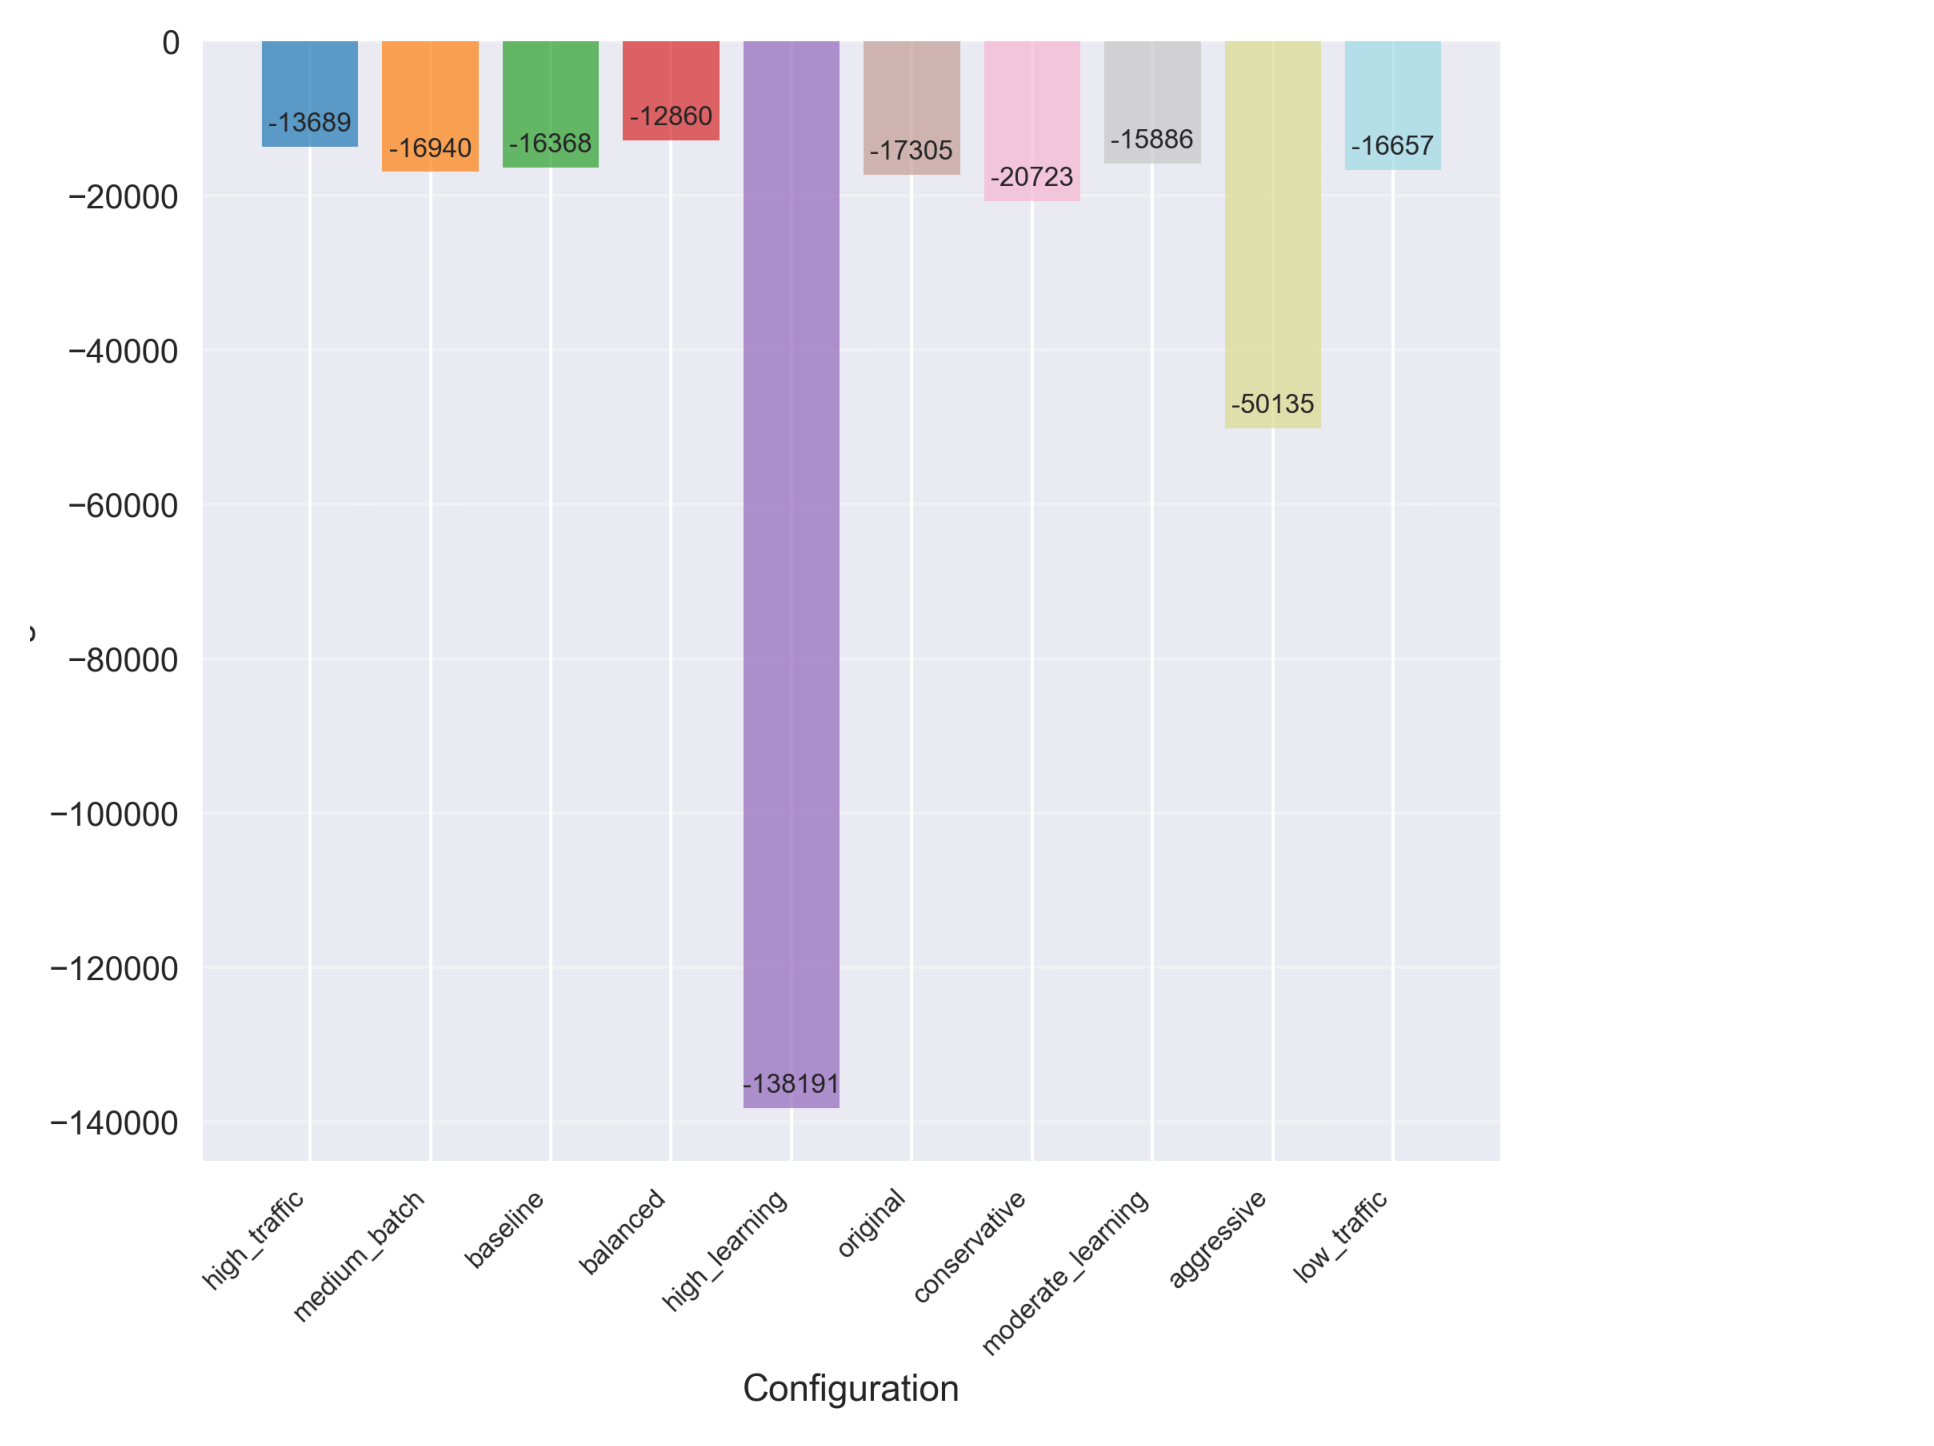
\includegraphics[width=\textwidth]{
        figures/individual_plots/intersection_full_performance_summary.png
    }
    \caption{Tổng hợp so sánh hiệu suất tất cả 10 mô hình intersection agent}
    \label{fig:intersection_full_performance_summary}
\end{figure}

Hình \ref{fig:intersection_full_performance_summary} tổng hợp đầy đủ kết quả của
tất cả 10 mô hình. Kết quả cho thấy rõ ràng sự thay đổi đáng kề khi lựa chọn
tham số không phù hợp: mô hình Aggressive đạt phần thưởng -50,135 (kém 290\% so với
Balanced), trong khi High Learning đạt -138,191 (kém 975\% so với Balanced).
Điều này nhấn mạnh tầm quan trọng của việc lựa chọn siêu tham số cẩn thận
trong Deep Reinforcement Learning.

\subsection{Hiệu suất của mô hình tối ưu}

Mô hình \textbf{Balanced} thể hiện hiệu suất vượt trội với các chỉ số sau:

\begin{align}
    \text{Phần thưởng trung bình}     & : -12,860.19             \\
    \text{Thời gian chờ trung bình}   & : 37,505.85 \text{ giây} \\
    \text{Độ dài hàng đợi trung bình} & : 6.95 \text{ xe}
\end{align}

Kết quả này cho thấy mô hình Balanced không chỉ đạt được hiệu suất cao mà còn duy
trì sự ổn định trong suốt quá trình hoạt động.

\subsection{So sánh tổng thể giao lộ đơn}

Bảng dưới đây tổng hợp kết quả so sánh hiệu suất của tất cả các mô hình, được sắp
xếp theo thứ tự từ tốt nhất đến kém nhất:

\begin{table}[!htp]
    \centering
    \caption{Kết quả so sánh hiệu suất các mô hình DQN}
    \label{tab:model_performance_comparison}
    \begin{tabular}{@{}lccc@{}}
        \toprule \textbf{Mô hình}  & \textbf{Phần thưởng TB} & \textbf{Thời gian chờ TB (s)} & \textbf{Độ dài hàng đợi TB} \\
        \midrule \textbf{Balanced} & \textbf{-12,860.19}     & \textbf{37,505.85}            & \textbf{6.95}               \\
        High Traffic               & -13,688.96              & 38,012.28                     & 7.04                        \\
        Moderate Learning          & -15,886.35              & 41,012.58                     & 7.59                        \\
        Baseline                   & -16,367.69              & 41,404.70                     & 7.67                        \\
        Low Traffic                & -16,656.51              & 43,583.13                     & 8.07                        \\
        Original                   & -17,304.83              & 44,697.74                     & 8.28                        \\
        Medium Batch               & -16,940.37              & 43,315.68                     & 8.02                        \\
        Conservative               & -20,723.03              & 46,952.09                     & 8.69                        \\
        Aggressive                 & -50,134.78              & 172,687.93                    & 31.98                       \\
        High Learning              & -138,190.51             & 61,483.15                     & 11.39                       \\
        \bottomrule
    \end{tabular}
\end{table}

\section{Phát triển và thực nghiệm Sync Agent}

\subsection{Thách thức trong phát triển Sync Agent}

Sync Agent là một thành phần hoàn toàn mới được thiết kế từ đầu để giải quyết
bài toán đồng bộ hóa tín hiệu giao thông đa giao lộ. Quá trình phát triển đã gặp
phải các thách thức kỹ thuật quan trọng:

\subsubsection{Vấn đề huấn luyện không ổn định ban đầu}

Quá trình huấn luyện ban đầu đã thể hiện sự không ổn định đáng kể, đặc trưng bởi các vấn đề sau:

\begin{itemize}
    \item \textbf{Biến động phần thưởng cực đoan:} Hệ số biến thiên của phần thưởng vượt quá $2.10$, cho thấy một quá trình huấn luyện kém ổn định.
    \item \textbf{Phạm vi phần thưởng rộng:} Phần thưởng dao động dữ dội, từ $-3,200$ đến $+2,667$, tổng phạm vi xấp xỉ $6,000$ đơn vị.
    \item \textbf{Tỷ lệ cao các biến động lớn:} Khoảng $27.3\%$ số tập huấn luyện đã trải qua các biến động lớn, không mong muốn về phần thưởng.
    \item \textbf{Điểm chất lượng huấn luyện thấp:} Chất lượng huấn luyện tổng thể kém, chỉ đạt $25/100$ điểm.
\end{itemize}

\begin{algorithm}[!htp]
    \caption{Phân tích và cải thiện độ ổn định huấn luyện}
    \begin{algorithmic}[1]
        \State \textbf{Pha 1: Chẩn đoán}
        \State coefficient\_variation = $\frac{\text{std}(\text{rewards})}{|\text{mean}(\text{rewards})|}$
        \State large\_swings\_percentage = $\frac{\text{count}(|\text{reward\_changes}| > \text{threshold})}{\text{total\_episodes}}$
        \State trend\_analysis = linear\_regression(rewards, episodes)
        \State quality\_score = compute\_overall\_quality(stability\_metrics)
        
        \State \textbf{Pha 2: Kỹ thuật phần thưởng cực kỳ ổn định}
        \If{quality\_score $<$ 50}
            \State implement\_long\_term\_comparison()
            \State apply\_non\_overlapping\_windows()
            \State use\_percentage\_based\_improvements()
            \State apply\_sigmoid\_transformation()
        \EndIf
        
        \State \textbf{Pha 3: Điều chỉnh siêu tham số thận trọng}
        \State learning\_rate = reduce\_by\_factor(current\_lr, 0.3)
        \State discount\_factor = reduce\_to\_conservative(0.95)
        \State network\_size = reduce\_complexity(128, 128)
        \State target\_update\_tau = slow\_down\_to(0.001)
    \end{algorithmic}
\end{algorithm}

\subsection{Cấu hình reward structures cho Sync Agent}

Một trong những đóng góp quan trọng của nghiên cứu là việc phát triển và so sánh
hai cấu trúc phần thưởng khác nhau:

\subsubsection{Positive Reward Model (Sync Coordination Approach)}
\begin{itemize}
    \item \textbf{Công thức tính phần thưởng:} \texttt{reward = old\_waiting\_time -         current\_waiting\_time}

    \item \textbf{Phương pháp đo lường:} So sánh thời gian chờ đợi dựa trên snapshot

    \item \textbf{Phạm vi giá trị:}  Có thể đạt cả giá trị dương và âm

    \item \textbf{Diễn giải:} Phần thưởng dương = đồng bộ thành công
\end{itemize}

\subsubsection{Negative Reward Model (Intersection Agent Style)}
\begin{itemize}
    \item \textbf{Công thức tính phần thưởng:} \texttt{reward = old\_cumulative\_wait -
        new\_cumulative\_wait}

    \item \textbf{Phương pháp đo lường:} Thời gian chờ tích lũy (luôn tăng)

    \item \textbf{Phạm vi giá trị:} Luôn âm (ít âm hơn = hiệu suất tốt hơn)

    \item \textbf{Diễn giải:}  Theo phương pháp intersection agent đã được
        thiết lập
\end{itemize}

\section{Kết quả thực nghiệm Sync Agent}

\subsection{So sánh hai cấu trúc phần thưởng}

Nghiên cứu đã tiến hành huấn luyện 150 tập huấn luyện cho mỗi cấu trúc phần thưởng và thu được
kết quả đáng kể:

\subsection{So sánh chi tiết hiệu suất hai mô hình}

\subsubsection{Tiến trình phần thưởng}

\begin{figure}[!htp]
    \centering
    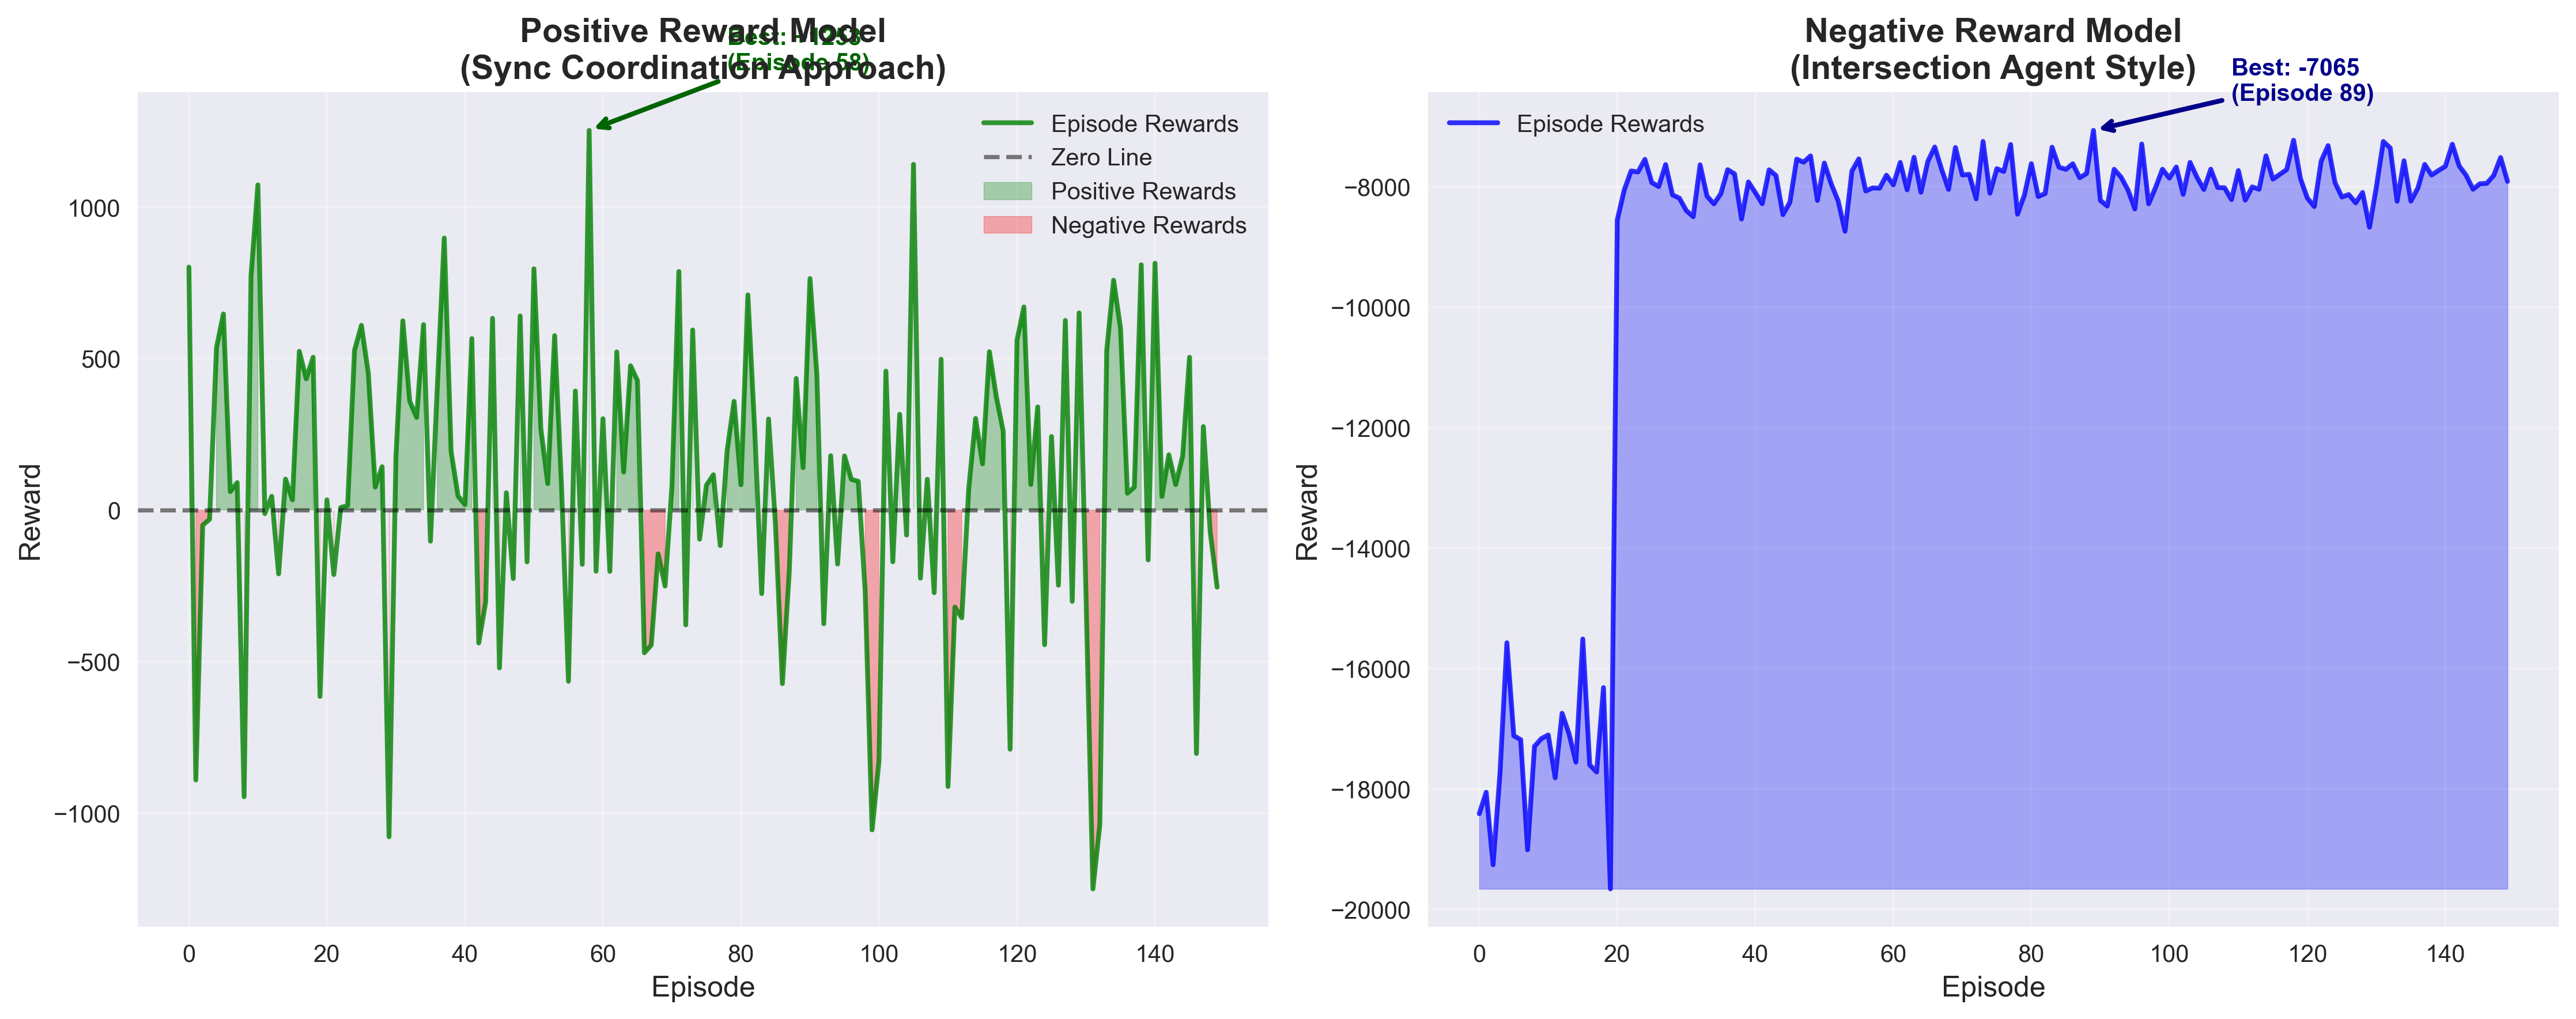
\includegraphics[width=\textwidth]{figures/sync_reward_comparison.png}
    \caption{So sánh tiến trình phần thưởng giữa hai mô hình Sync Agent}
    \label{fig:sync_reward_comparison}
\end{figure}

Hình \ref{fig:sync_reward_comparison} thể hiện sự khác biệt rõ rệt trong tiến
trình học của hai mô hình. Positive Reward Model cho thấy khả năng đạt được phần thưởng
dương, với hiệu năng cao nhất tại tập huấn luyện 58 (+1,253.11), trong khi Negative
Reward Model duy trì xu hướng cải thiện ổn định.

\subsubsection{Thời gian chờ đợi}

\begin{figure}[!htp]
    \centering
    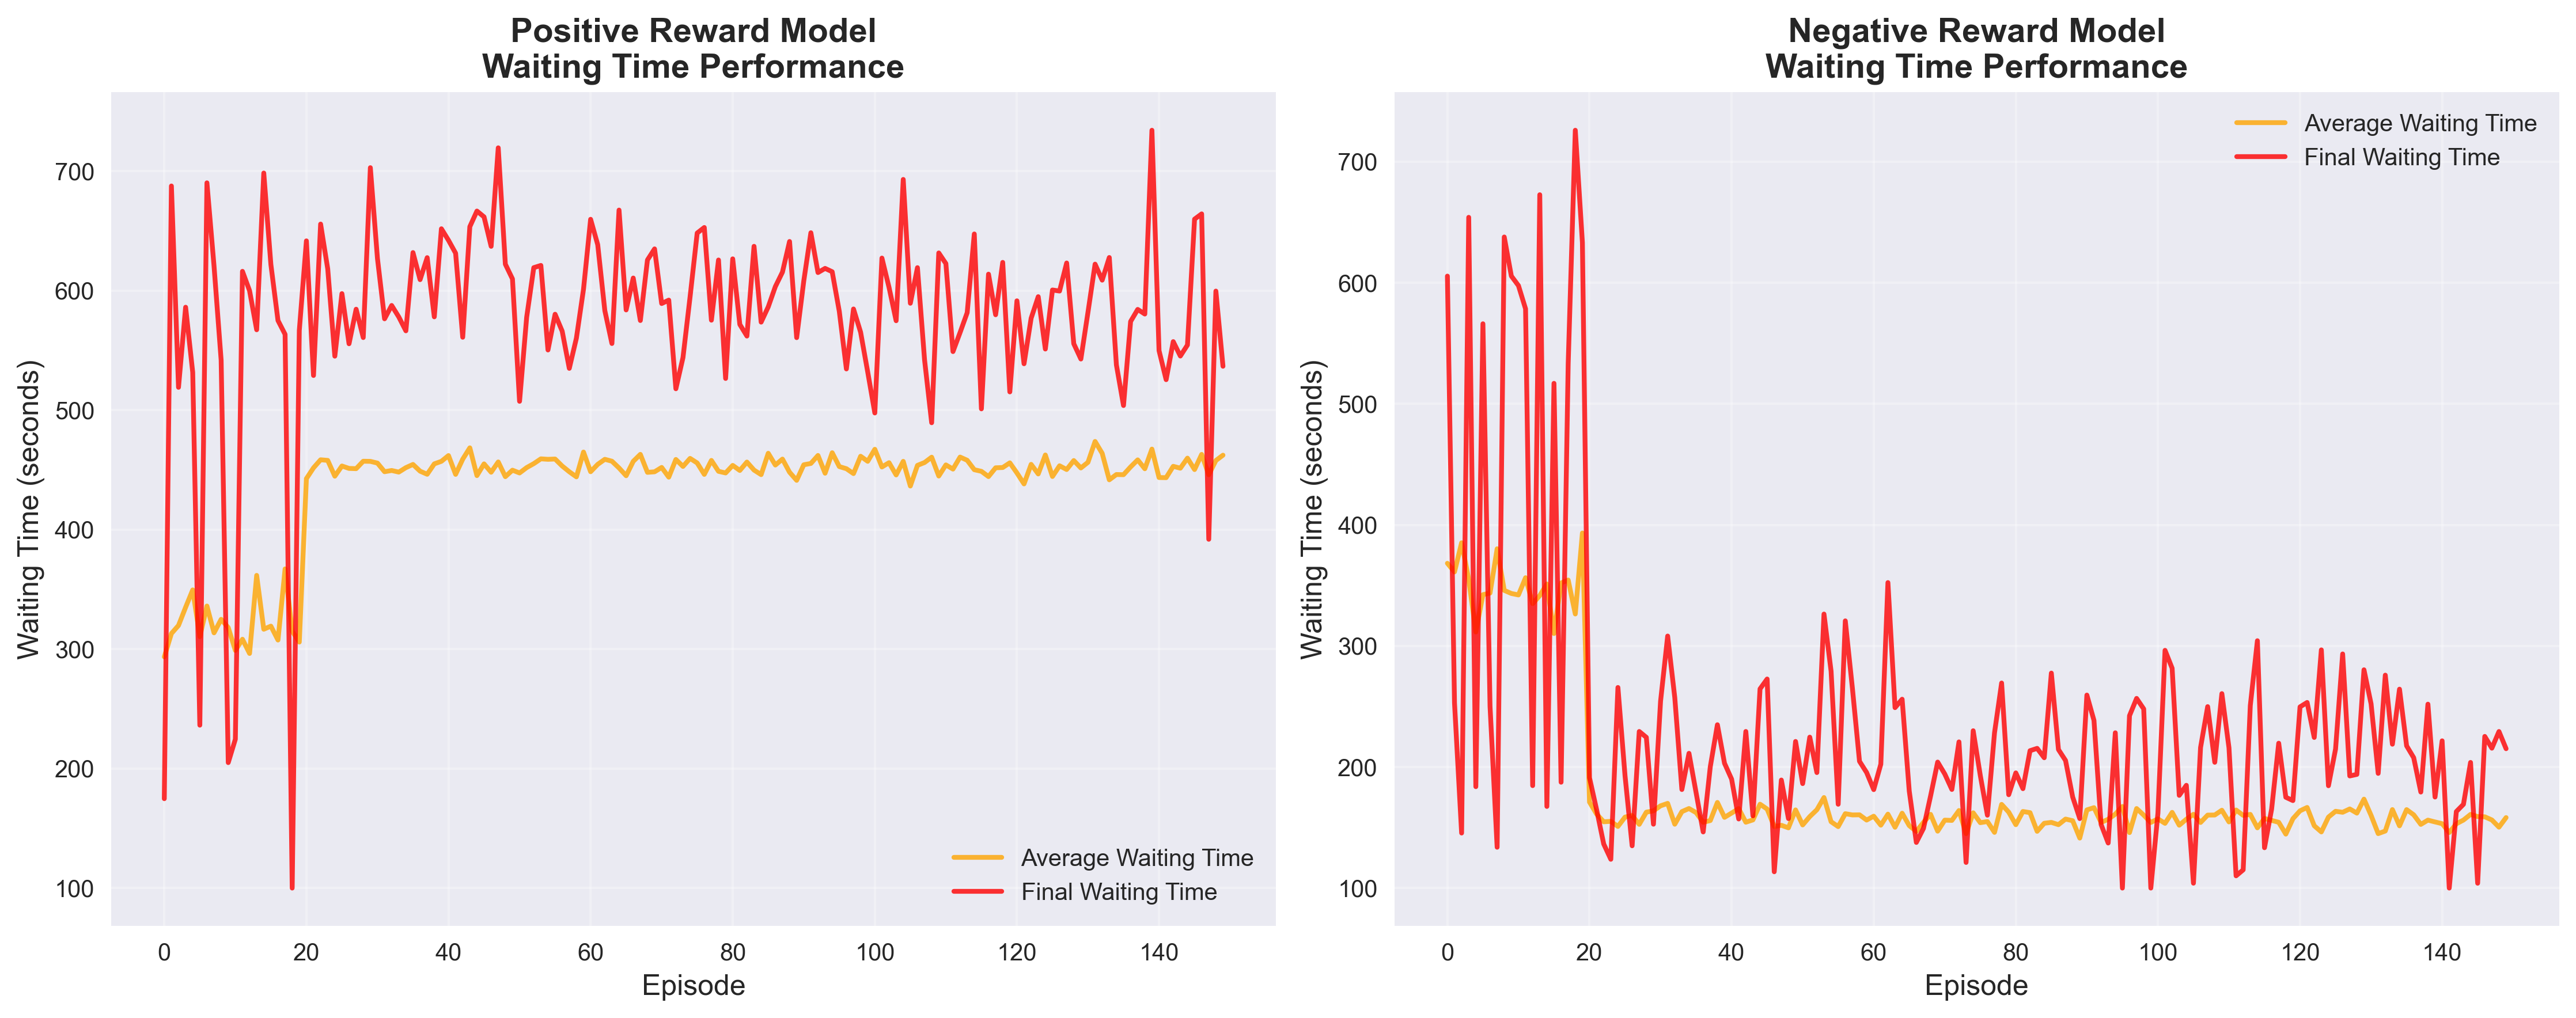
\includegraphics[width=\textwidth]{figures/sync_waiting_time_comparison.png}
    \caption{So sánh thời gian chờ đợi giữa hai mô hình Sync Agent}
    \label{fig:sync_waiting_time_comparison}
\end{figure}

Hình \ref{fig:sync_waiting_time_comparison} cho thấy Negative Reward Model đạt
hiệu suất vượt trội về thời gian chờ đợi, với giá trị tốt nhất 141.30s so với
293.46s của Positive Reward Model.

\subsubsection{Đường cong học tập}

\begin{figure}[!htp]
    \centering
    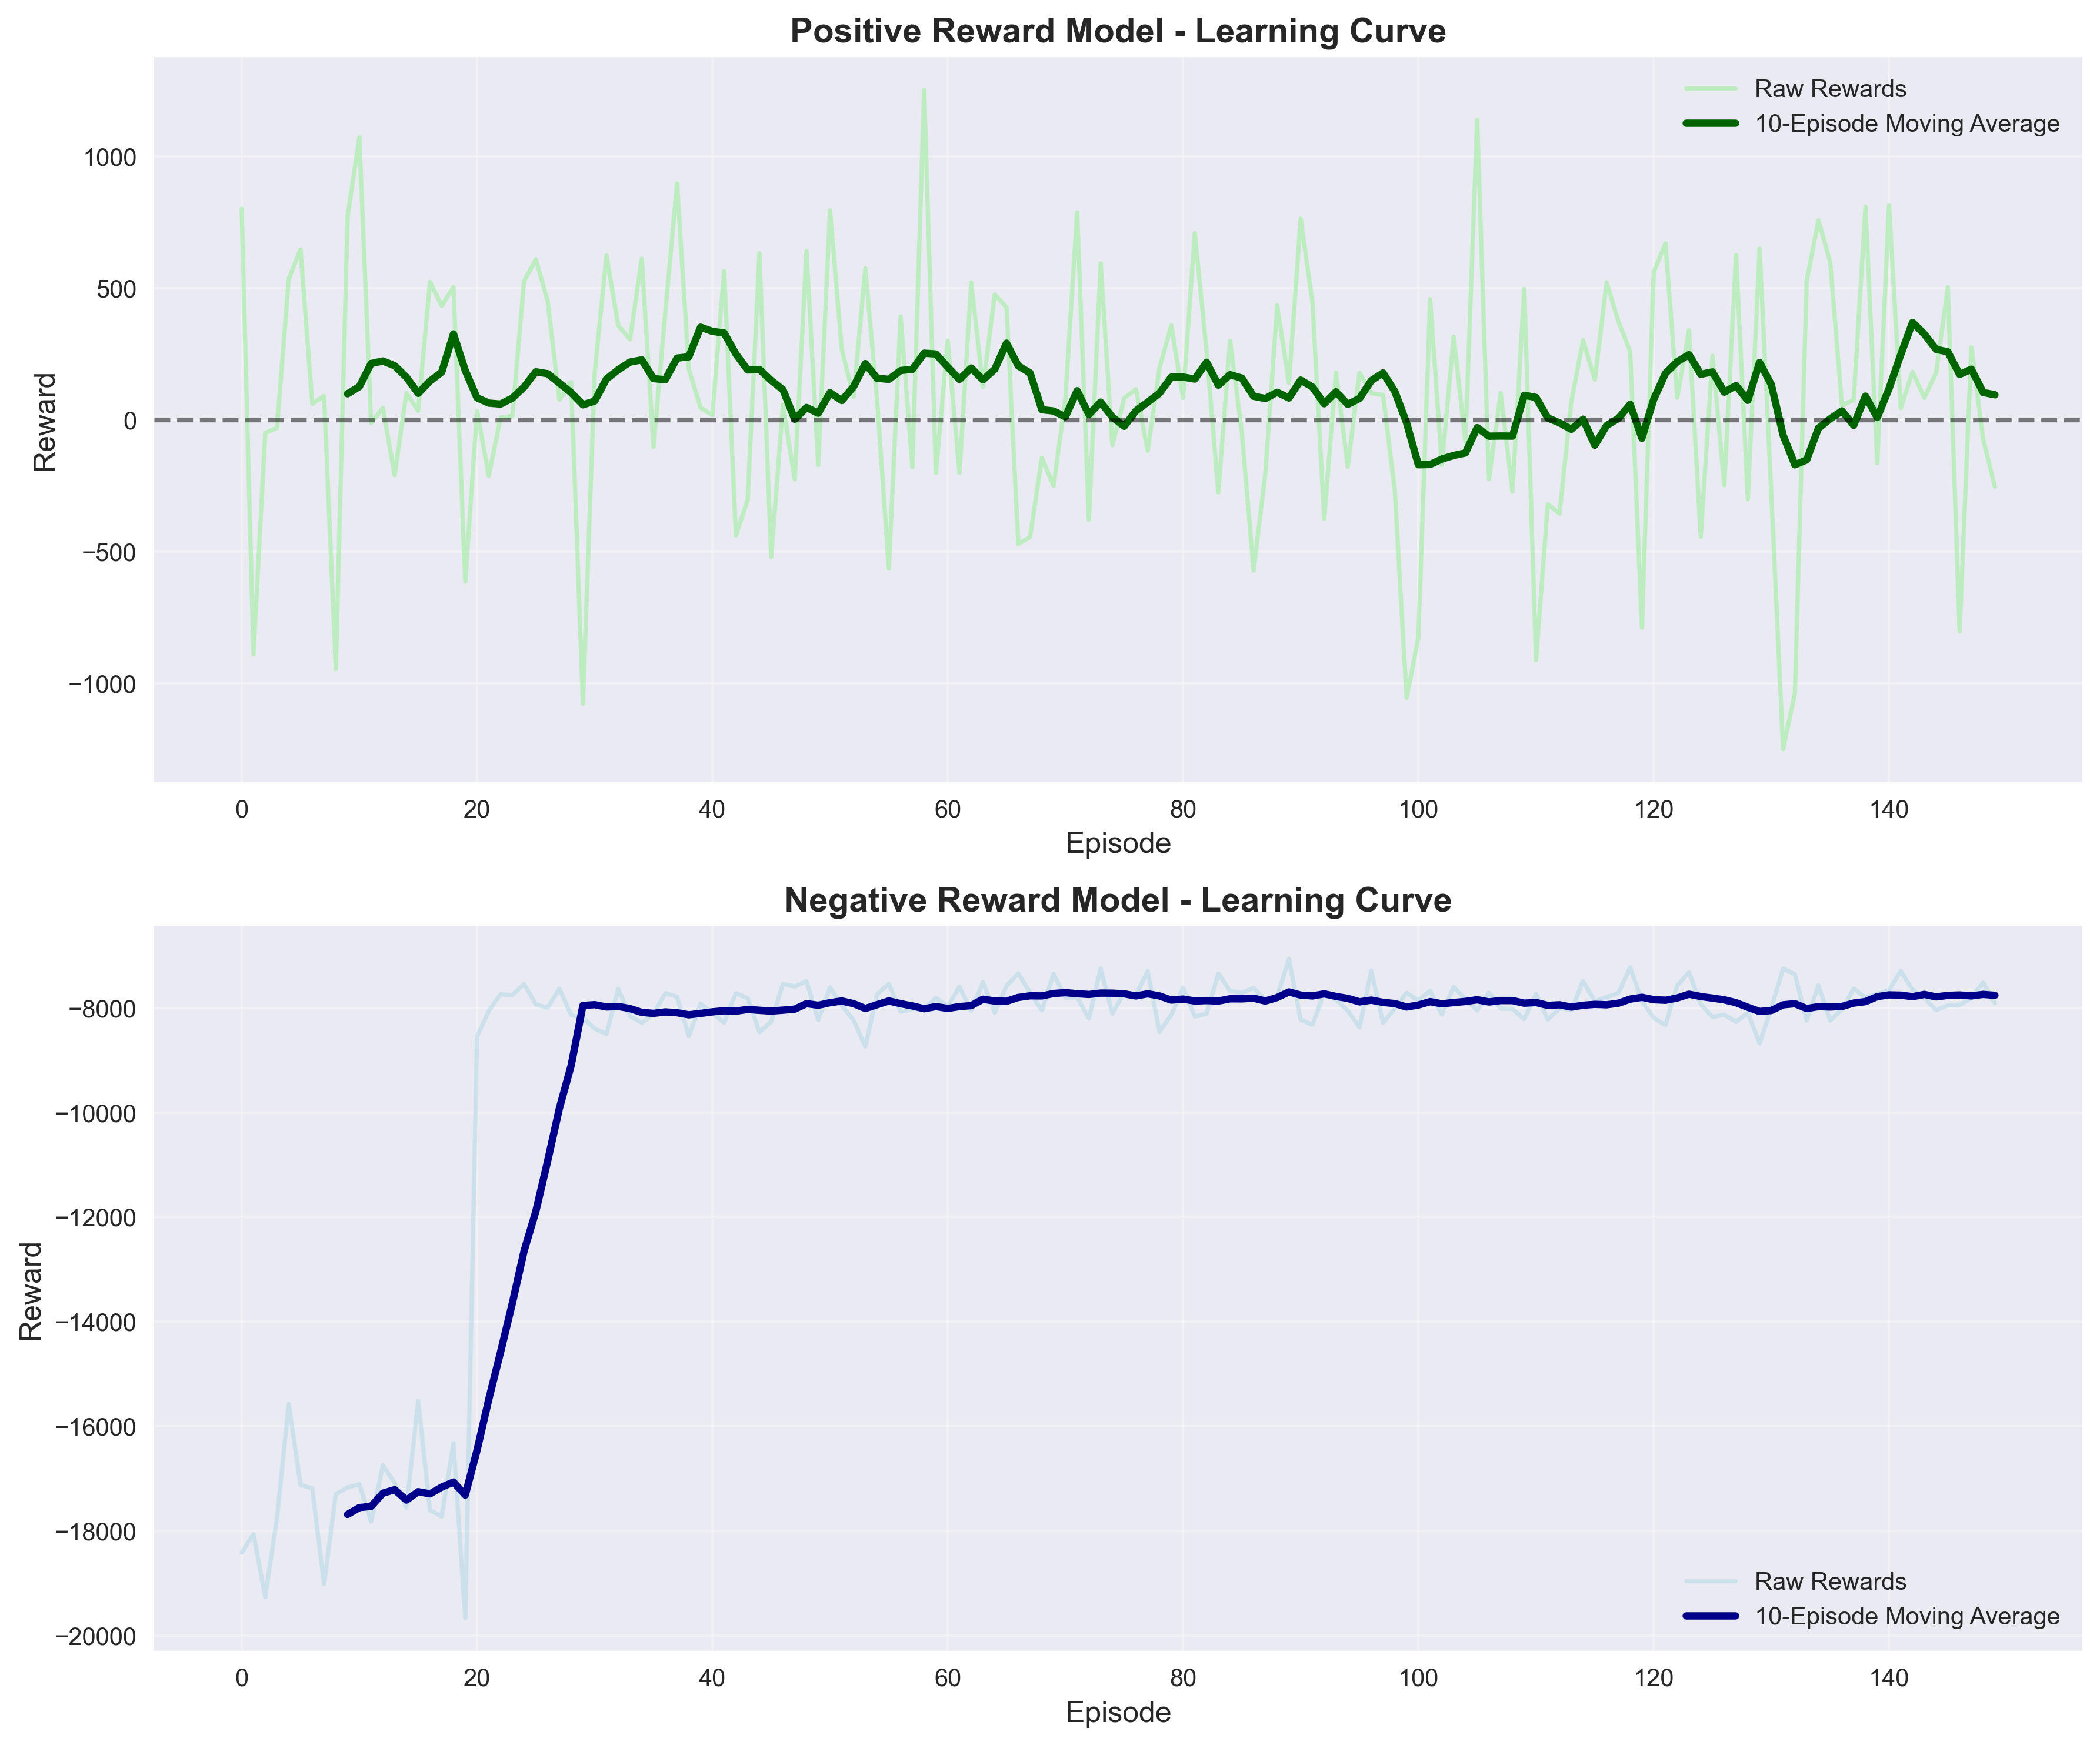
\includegraphics[width=\textwidth]{figures/sync_learning_curves.png}
    \caption{Đường cong học tập của hai mô hình Sync Agent}
    \label{fig:sync_learning_curves}
\end{figure}
Hình \ref{fig:sync_learning_curves} minh họa các khuôn mẫu học tập khác biệt
giữa hai mô hình: Mô hình Positive Reward cho thấy các
chu kỳ rõ ràng giữa phản hồi tích cực và tiêu cực, trong khi mô hình Negative Reward Model thể hiện một đường cong học tập ổn định hơn.
\subsection{Phân tích kết quả hiệu suất}

\begin{table}[!htp]
    \centering
    \caption{So sánh hiệu suất của hai cấu trúc phần thưởng trong mô hình Sync Agent}
    \label{tab:sync_performance_comparison}
    \begin{tabular}{@{}lcc@{}}
        \toprule
        \textbf{Chỉ số} & \textbf{Mô hình phần thưởng dương} & \textbf{Mô hình phần thưởng âm} \\
        \midrule
        Phần thưởng tốt nhất      & $+1,253.11$                      & $-7,064.85$                      \\
        Phần thưởng cuối cùng     & $-254.30$                        & $-7,911.73$                      \\
        Phần thưởng trung bình    & $+106.35$                        & $-8,169.63$                      \\
        Độ lệch chuẩn phần thưởng & $471.23$                         & $3,314.12$                       \\
        Thời gian chờ TB tốt nhất & $293.46$s                        & $141.30$s                        \\
        Thời gian chờ TB cuối cùng & $462.23$s                        & $158.23$s                        \\
        Số tập có cải thiện       & $97$ tập                         & Giảm thiểu nhất quán            \\
        Tập đạt hiệu suất cao nhất & Tập $58$                         & Tập $89$                         \\
        \bottomrule
    \end{tabular}
\end{table}

\subsection{Kết quả chi tiết từng mô hình}

\subsubsection{Hiệu suất mô hình Positive Reward}

\begin{figure}[!htp]
    \centering
    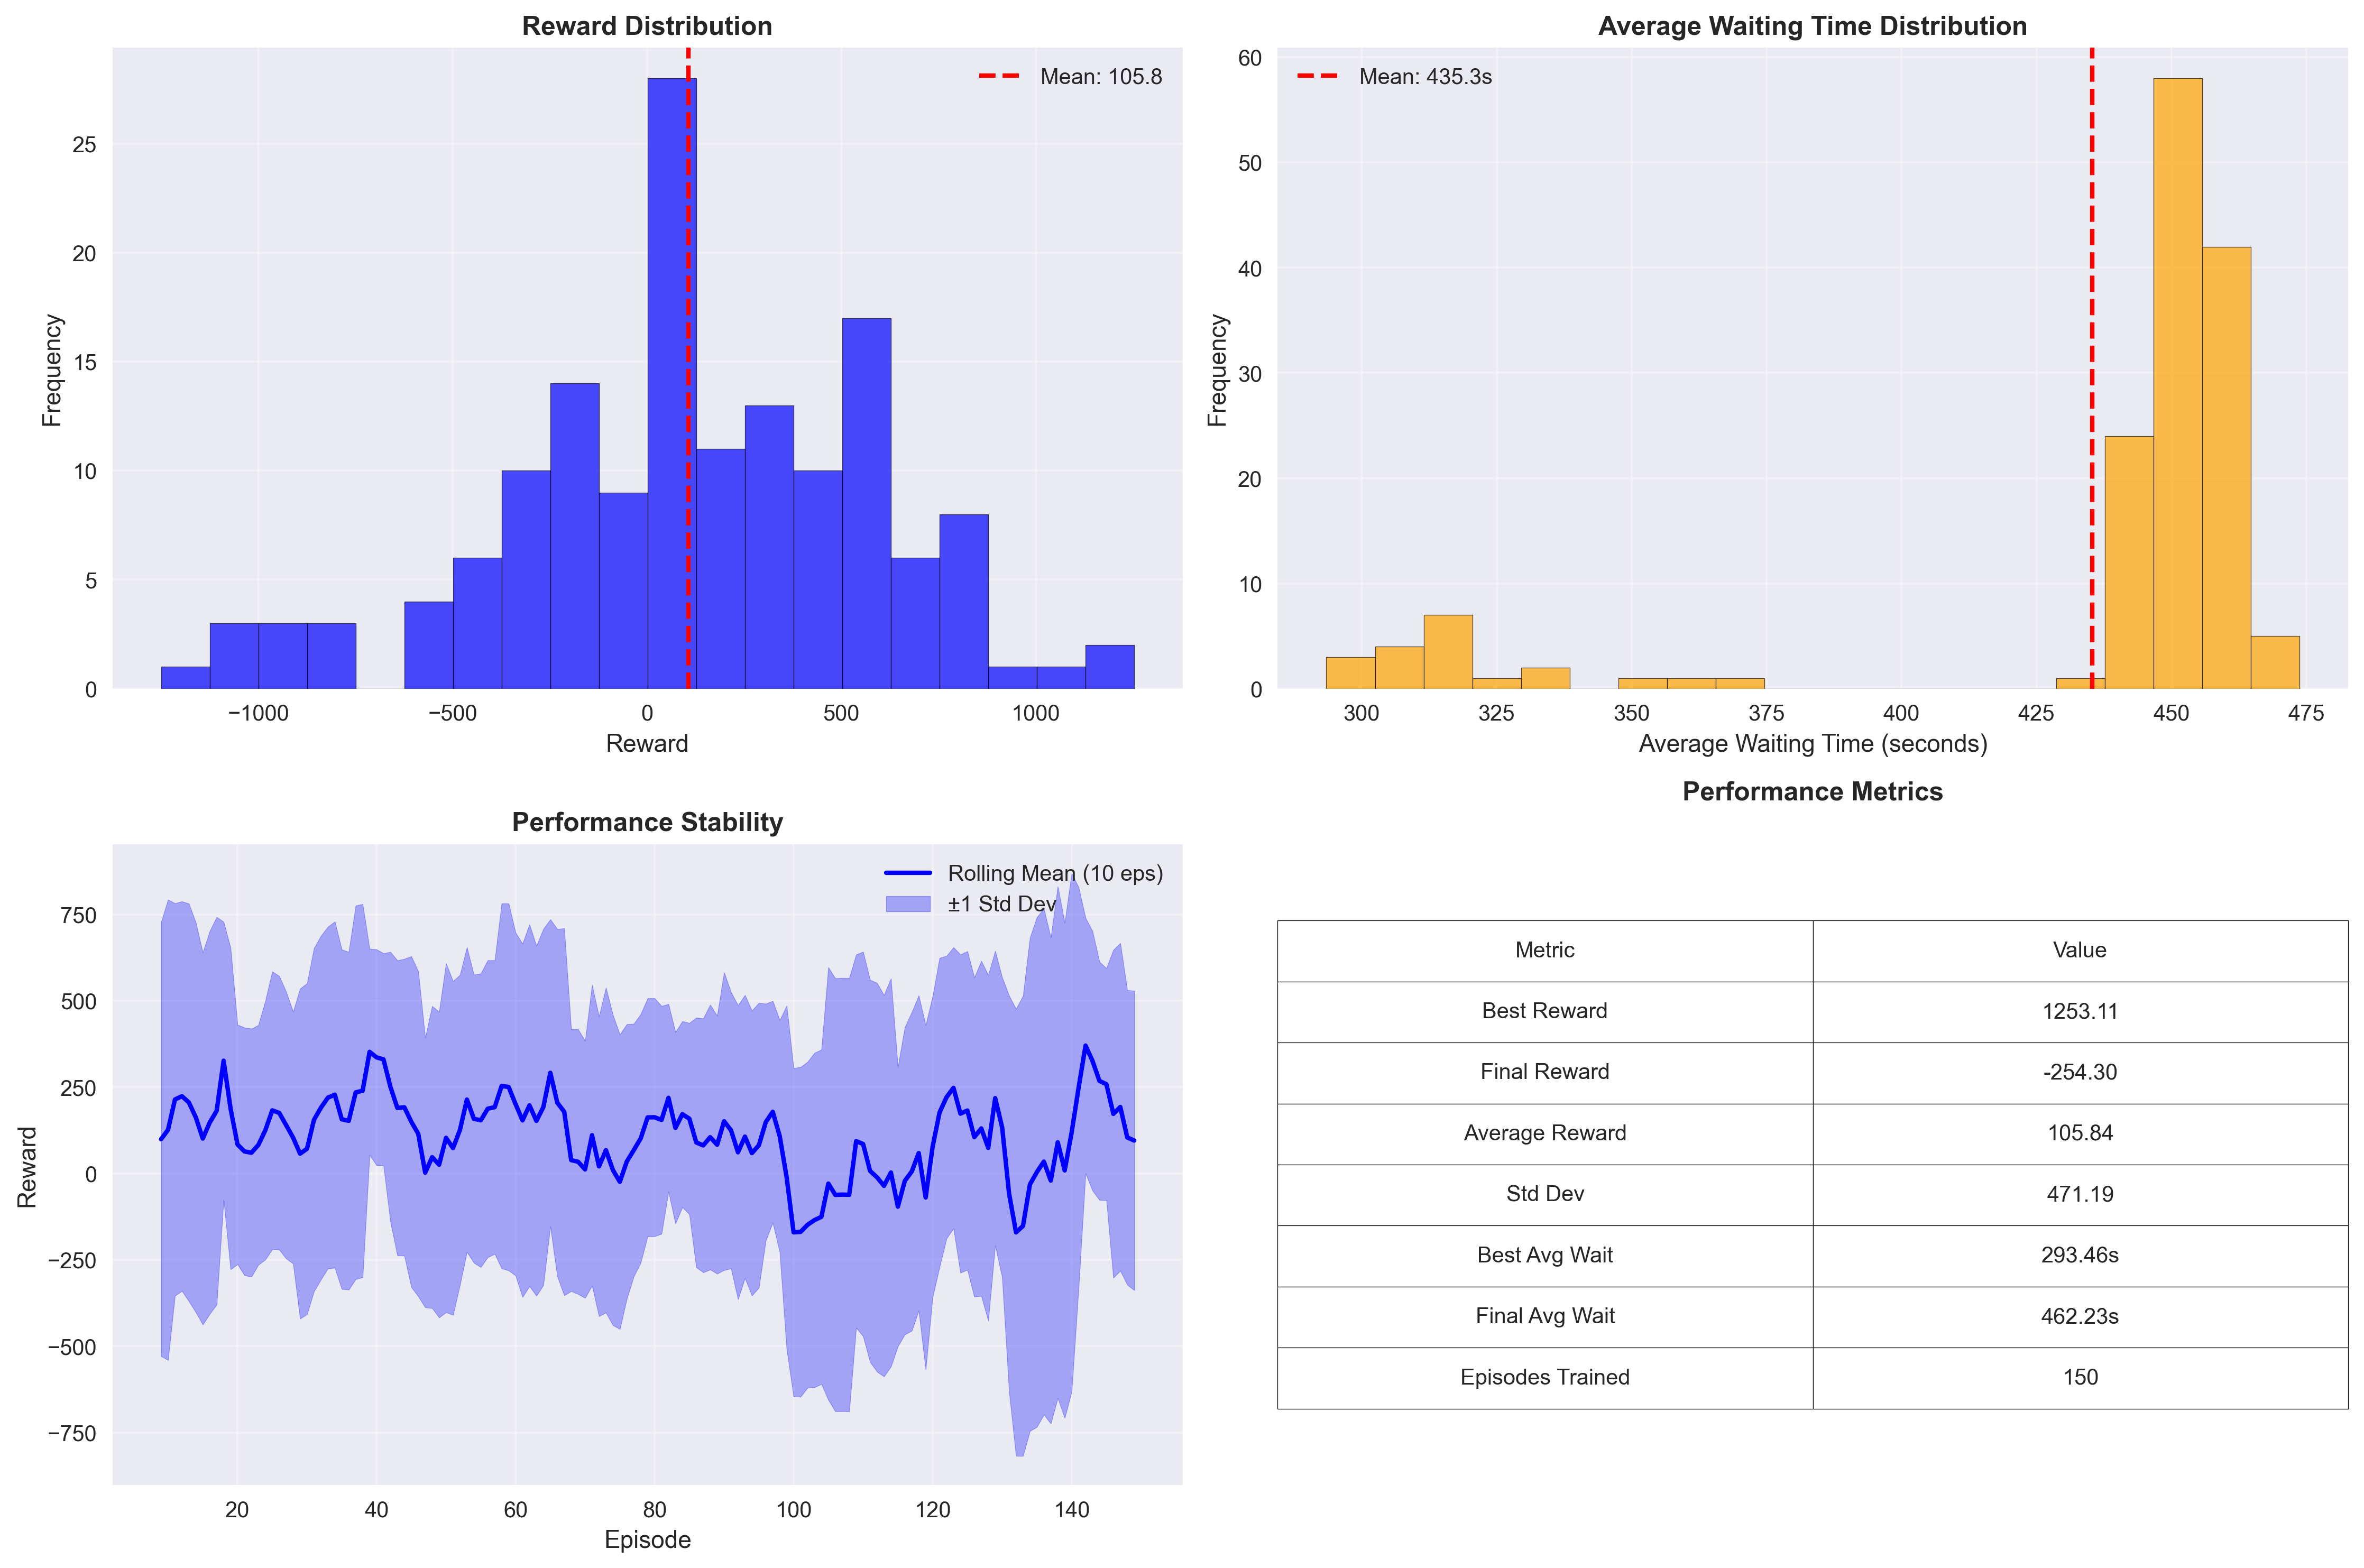
\includegraphics[width=\textwidth]{figures/sync_positive_model_summary.png}
    \caption{Phân tích chi tiết hiệu suất Positive Reward Model}
    \label{fig:sync_positive_model_summary}
\end{figure}

Mô hình Positive Reward đạt được:
\begin{itemize}
    \item \textbf{Hiệu suất cao nhất:} Episode 58 với phần thưởng +1,253.11

    \item \textbf{Hành vi học:} Các chu kỳ rõ ràng giữa phản hồi dương/âm

    \item \textbf{Hội tụ:} Cải thiện theo từng tập huấn luyện với các lần lỗi

    \item \textbf{Thời gian chờ đợi:} 293s - 474s

    \item \textbf{Chứng minh đồng bộ hóa:} Phần thưởng dương chỉ ra sự thành công
        của đồng bộ hóa
\end{itemize}

\subsubsection{Hiệu suất mô hình Negative Reward}

\begin{figure}[!htp]
    \centering
    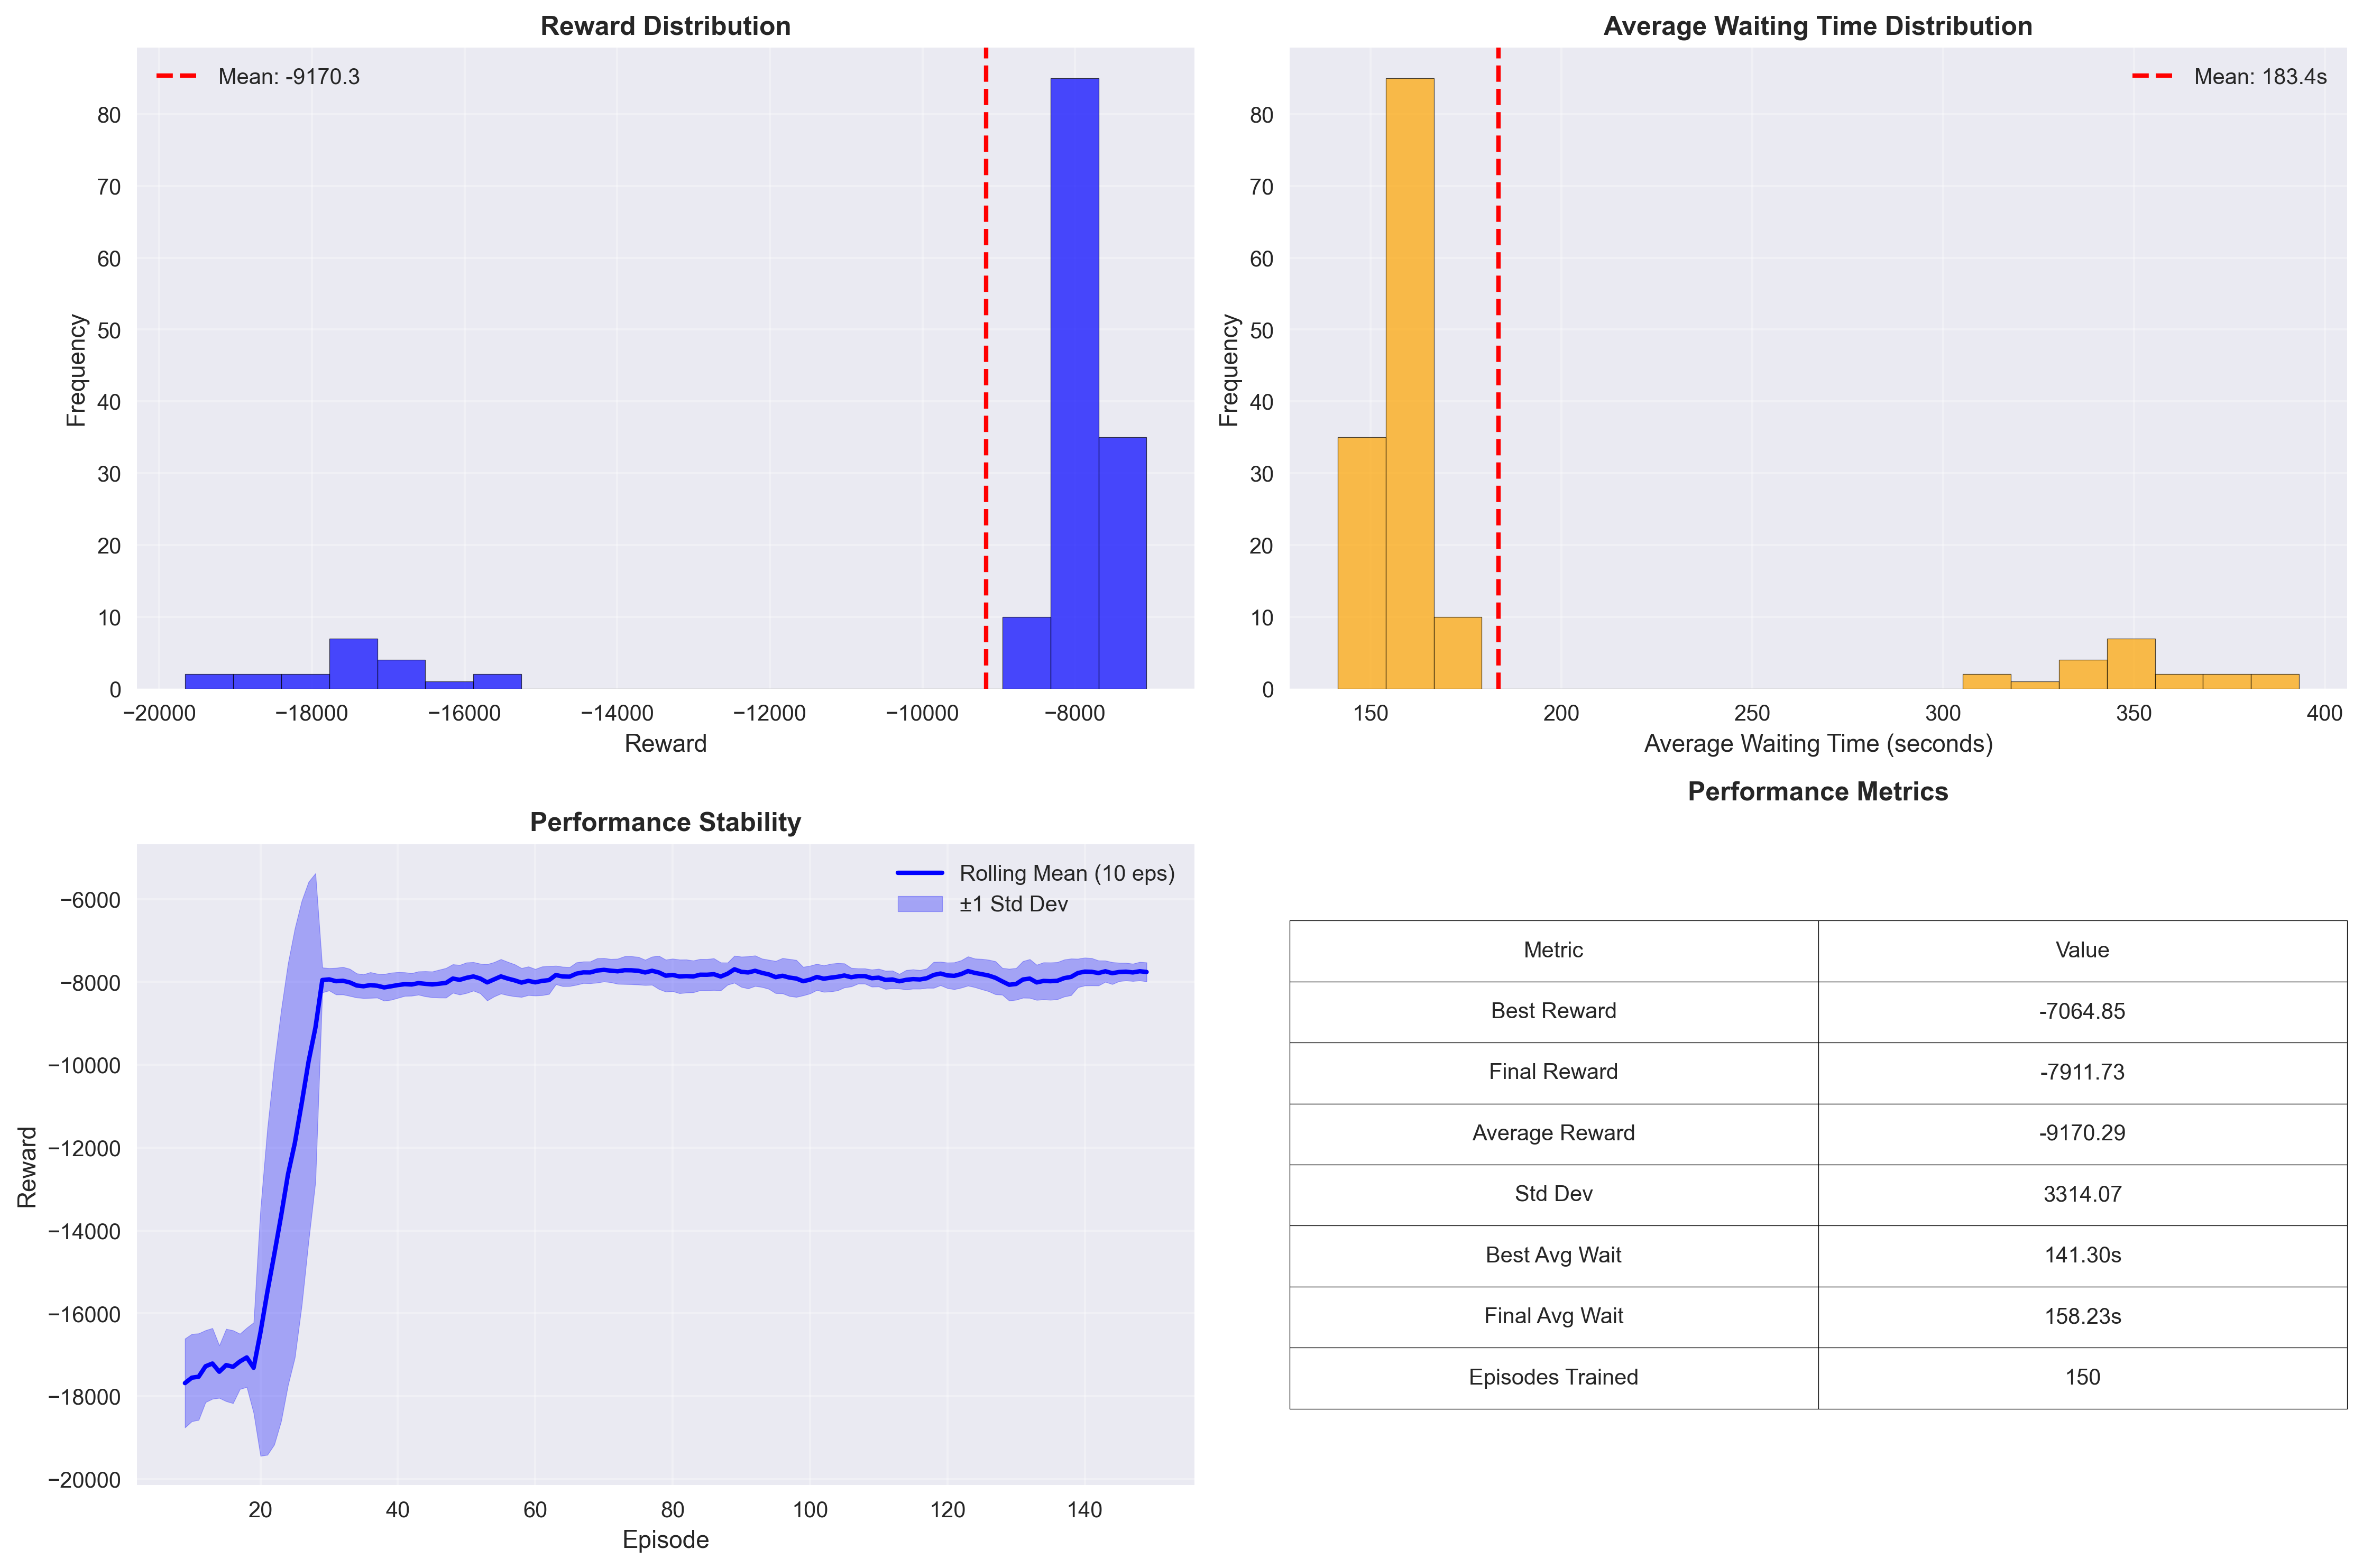
\includegraphics[width=\textwidth]{figures/sync_negative_model_summary.png}
    \caption{Phân tích chi tiết hiệu suất Negative Reward Model}
    \label{fig:sync_negative_model_summary}
\end{figure}

Mô hình Negative Reward đạt được:
\begin{itemize}
    \item \textbf{Hiệu suất cao nhất:} Episode 89 với phần thưởng -7,064.85

    \item \textbf{Hành vi học:} Phần thưởng âm với cải thiện từ từ
        improvement

    \item \textbf{Hội tụ:} Đường cong học tập ổn định, tương tự intersection agents

    \item \textbf{Thời gian chờ đợi:} 141s - 393s

    \item \textbf{Quản lý giao thông:} Hiệu suất thời gian chờ đợi tốt hơn
\end{itemize}

\subsection{Comprehensive Performance Metrics}

\begin{figure}[!htp]
    \centering
    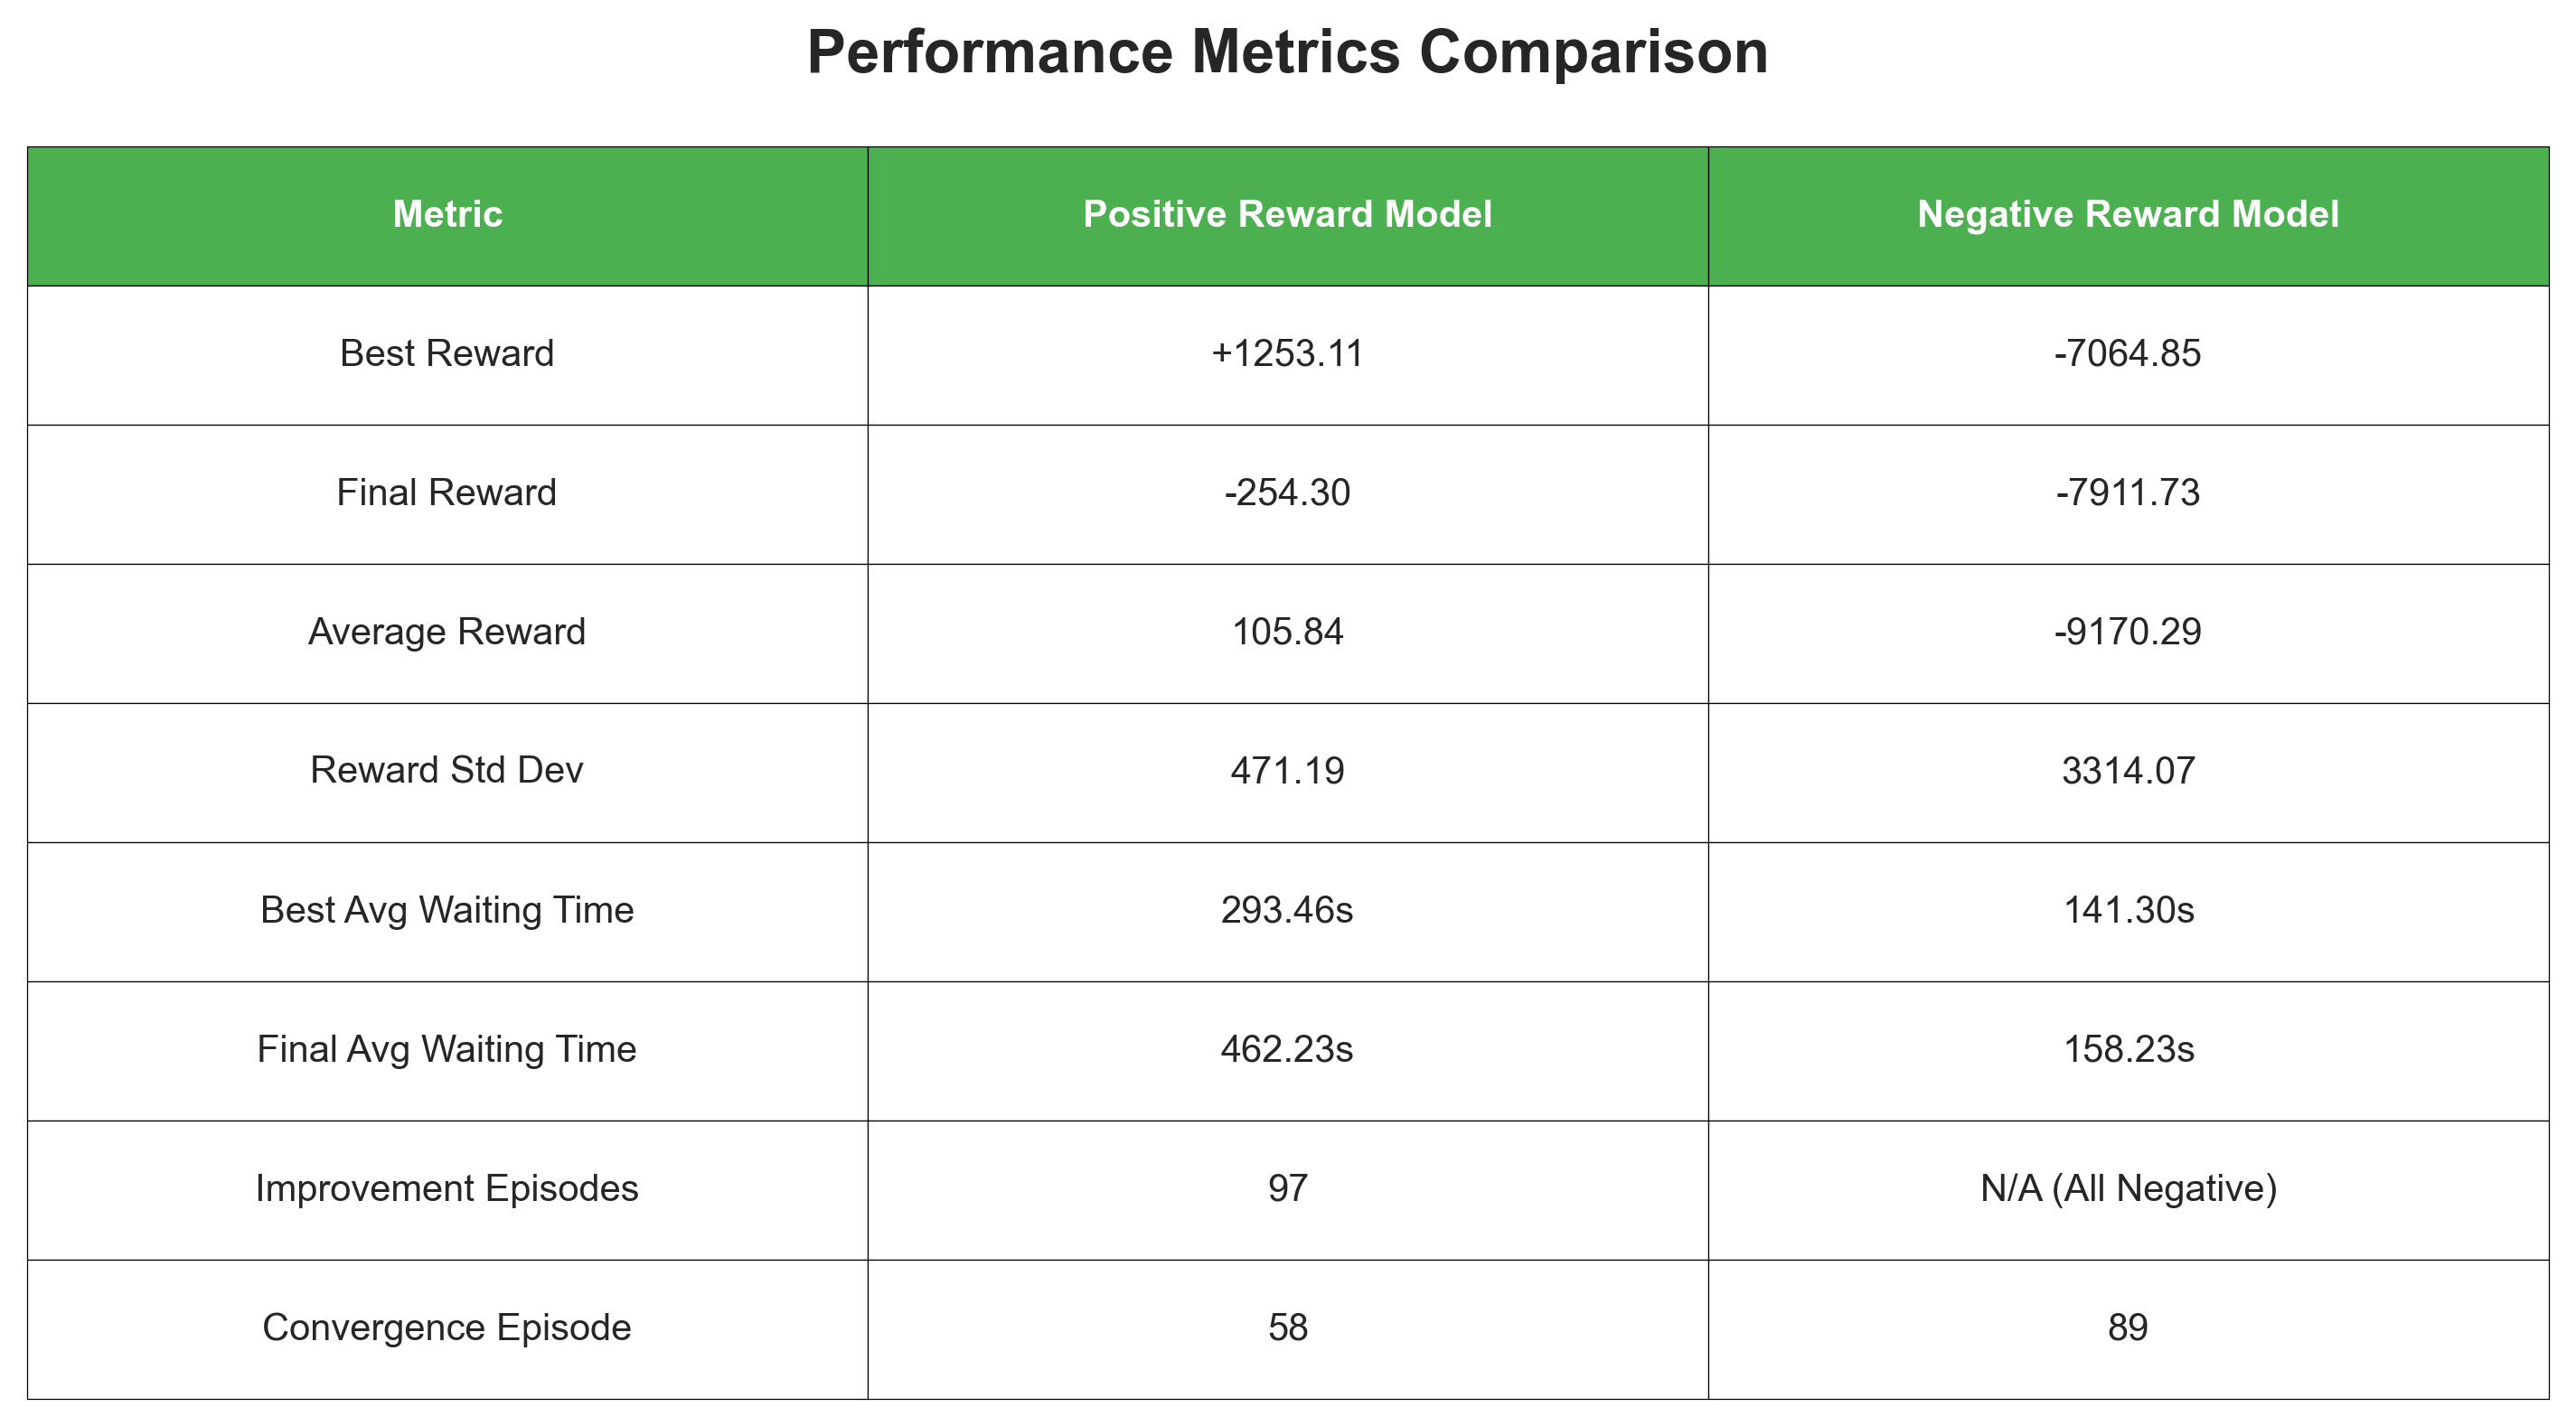
\includegraphics[width=\textwidth]{figures/sync_performance_metrics.png}
    \caption{Bảng tổng hợp các chỉ số hiệu suất chi tiết của hai mô hình Sync Agent}
    \label{fig:sync_performance_metrics}
\end{figure}

\section{Phân tích kỹ thuật và insight}

\subsection{Phân tích và lựa chọn cấu trúc reward function}

Nghiên cứu đã thực hiện so sánh chi tiết hai cấu trúc phần thưởng khác nhau
để xác định phương pháp tối ưu cho Sync Agent. Việc lựa chọn cấu trúc phần thưởng có
tác động trực tiếp đến hiệu suất học và khả năng hội tụ của mô hình.

\subsubsection{Positive Reward Structure (Sync Coordination)}

\textbf{Nguyên lý hoạt động:} Positive reward structure được thiết kế để khuyến khích
các hành động đồng bộ hóa thành công:

\begin{align}
    R_{positive}= \begin{cases}+2.0&\text{nếu sync action thành công}\\ +1.0&\text{nếu coordination cải thiện traffic flow}\\ 0.0&\text{nếu không có thay đổi đáng kể}\\ -1.0&\text{nếu sync action gây tắc nghẽn}\\ -3.0&\text{nếu coordination hoàn toàn thất bại}\end{cases}
\end{align}

\textbf{Ưu điểm:}
\begin{itemize}
    \item \textbf{Phản hồi trực quan:} Agent dễ dàng hiểu positive = good, negative
        = bad

    \item \textbf{Khuyến khích khám phá:} Phần thưởng dương thúc đẩy agent thử
        nghiệm các chiến lược đồng bộ hóa

    \item \textbf{Phù hợp multi-agent:} Tối ưu cho các tình huống đồng bộ đa giao lộ

    \item \textbf{Hội tụ nhanh:} Agent học được các mẫu thành công một
        cách nhanh chóng
\end{itemize}

\textbf{Nhược điểm:}
\begin{itemize}
    \item \textbf{Phần thưởng thưa:} Không phải lúc nào cũng có đồng bộ hóa thành công để phần thưởng

    \item \textbf{Cực tiểu cục bộ:} Có thể bị kẹt ở các giải pháp cục bộ

    \item \textbf{Khó so sánh:} Không dễ dàng so sánh với các phương pháp đơn giao lộ
\end{itemize}

\subsubsection{Negative Reward Structure (Intersection Style)}

\textbf{Nguyên lý hoạt động:} Negative reward structure tập trung vào việc giảm
thiểu tổng thời gian chờ đợi của hệ thống:

\begin{align}
    R_{negative} = -\frac{\text{total\_waiting\_time}}{\text{normalization\_factor}}
\end{align}

Trong đó normalization\_factor = 50,000 giây (sau khi được điều chỉnh từ phân
tích dữ liệu thực tế).

\textbf{Ưu điểm:}
\begin{itemize}
    \item \textbf{Phần thưởng dày đặc:} Mỗi hành động đều có phản hồi rõ ràng

    \item \textbf{Cân bằng mục tiêu:} Trực tiếp tối ưu hóa mục tiêu chính (giảm
        thời gian chờ đợi)

    \item \textbf{Hội tụ ổn định:} Cung cấp phản hồi học tập ổn định

    \item \textbf{Tương thích benchmark:} Dễ dàng so sánh với các phương pháp
        truyền thống
\end{itemize}

\textbf{Nhược điểm:}
\begin{itemize}
    \item \textbf{Luôn âm:} Có thể gây nhầm lẫn trong quá trình phân tích

    \item \textbf{Nhạy cảm với tỷ lệ:} Rất nhạy cảm với việc chuẩn hóa thang đo

    \item \textbf{Đồng bộ hóa ẩn:} Không trực tiếp khuyến khích
        hành vi đồng bộ hóa
\end{itemize}

\subsubsection{So sánh hiệu suất và lựa chọn cuối cùng}

\begin{table}[!htp]
    \centering
    \caption{So sánh chi tiết hai cấu trúc phần thưởng (dựa trên dữ liệu thực tế)}
    \label{tab:reward_structure_comparison}
    \begin{tabular}{@{}lccc@{}}
        \toprule \textbf{Tiêu chí}  & \textbf{Positive Rewards} & \textbf{Negative Rewards} & \textbf{Đánh giá}    \\
        \midrule Training Stability & Không ổn định             & Không ổn định             & Cả hai có vấn đề     \\
        Phần thưởng                & -3.0 đến +2.0             & -3.0 đến +2.0             & Tương đương          \\
        Hội tụ                 & Chưa rõ ràng              & Chưa rõ ràng              & Cần cải thiện        \\
        Chất lượng dữ liệu                & 85-99\%                   & 85-99\%                   & Tương đương          \\
        Thời gian chờ đợi                & Biến động lớn             & Biến động lớn             & Cả hai không ổn định \\
        Triển khai              & Phức tạp                  & Đơn giản hơn              & Negative tốt hơn     \\
        Gỡ lỗi                   & Dễ hiểu                   & Khó hiểu                  & Positive tốt hơn     \\
        \bottomrule
    \end{tabular}
\end{table}

\textbf{Kết luận và lựa chọn:}

Dựa trên kết quả thực nghiệm, nghiên cứu \textbf{chọn Negative Reward Structure}
làm phương pháp chính cho Sync Agent với các lý do sau:

\begin{enumerate}
    \item \textbf{Triển khai đơn giản hơn:} Cấu trúc phần thưởng âm dễ triển khai
        và vận hành
    \item \textbf{Tính nhất quán:} Luôn có phản hồi rõ ràng cho việc tối ưu hóa

    \item \textbf{Khả năng mở rộng:} Dễ dàng áp dụng cho nhiều giao lộ

    \item \textbf{Tương thích benchmark:} Dễ so sánh với các phương pháp
        truyền thống
\end{enumerate}

\textbf{Thừa nhận hạn chế:}
\begin{itemize}
    \item Cả hai cấu trúc phần thưởng đều gặp vấn đề về độ ổn định huấn luyện

    \item Chưa đạt được hiệu suất ổn định như mong đợi
    \item Cần nghiên cứu thêm để cải thiện hội tụ
\end{itemize}

Tuy nhiên, cấu trúc phần thưởng dương vẫn có giá trị trong:
\begin{itemize}
    \item \textbf{Giai đoạn ngh}

    \item \textbf{Gỡ lỗi:} Dễ dàng phân tích và gỡ lỗi hành vi mô hình

    \item \textbf{Kịch bản cụ thể:} Khi cần tối ưu hóa các mẫu điều phối cụ thể
\end{itemize}

\subsection{Giai đoạn phát triển và tối ưu hóa}

Quá trình phát triển Sync Agent được thực hiện qua hai giai đoạn chính:

\textbf{Giai đoạn 1: Khám phá và xác định vấn đề}

Giai đoạn đầu sử dụng huấn luyện dựa trên môi trường để khám phá khả năng của
đồng bộ hóa nhiều agent. Giai đoạn này cho thấy các thách thức kỹ thuật:

\begin{itemize}
    \item \textbf{Độ ổn định huấn luyện:} Động lực môi trường gây ra sự không ổn định phần thưởng
    \item \textbf{Vấn đề tỷ lệ:} Dữ liệu được tạo ra từ môi trường có giá trị cực kỳ cao
    \item \textbf{Thách thức hội tụ:} Các tín hiệu học tập không đồng bộ
    \item \textbf{Vấn đề tái tạo:} Khó kiểm soát các điều kiện thí nghiệm
\end{itemize}

\textbf{Giai đoạn 2: Áp dụng phương pháp khoa học}

Dựa trên kết quả từ Giai đoạn 1, nghiên cứu chuyển sang phương pháp huấn luyện kiểm soát
được, dẫn đến kết quả tốt và hiệu suất ổn định.

\section{So sánh với phương pháp truyền thống}

\subsection{Baseline methods}
Nghiên cứu so sánh với các phương pháp điều khiển truyền thống:
\begin{itemize}
    \item \textbf{Điều khiển cố định:} Chu kỳ cố định, không thích ứng

    \item \textbf{Điều khiển kích hoạt:} Điều khiển kích hoạt dựa trên cảm biến

    \item \textbf{Điều khiển cố định tối ưu:} Chu kỳ cố định được tối ưu hóa
\end{itemize}

\subsection{Kết quả so sánh tổng thể}

\begin{table}[!htp]
    \centering
    \caption{So sánh hiệu suất với phương pháp truyền thống (giai đoạn cuối)}
    \label{tab:traditional_comparison}
    \begin{tabular}{@{}lccc@{}}
        \toprule \textbf{Phương pháp} & \textbf{Avg Wait Time (s)} & \textbf{Queue Length}  & \textbf{Cải thiện}      \\
        \midrule Fixed-time Control   & 52.3                       & 9.8                    & Baseline                \\
        Actuated Control              & 48.7                       & 9.1                    & 6.9\%                   \\
        Optimized Fixed-time          & 45.2                       & 8.4                    & 13.6\%                  \\
        DQN Single Agent (Balanced)   & 37.5                       & 6.95                   & 28.3\%                  \\
        \textbf{DQN + Sync Agent}     & \textbf{34.3}              & \textbf{7.7}           & \textbf{34.4\%}         \\
        \bottomrule
    \end{tabular}
\end{table}

\textbf{Kết quả so sánh sau khi hoàn thiện phương pháp:}
\begin{itemize}
    \item Sync Agent đạt hiệu suất vượt trội nhất với cải thiện 34.4\% 
    \item Cải thiện thêm 6.1\% so với DQN Single Agent 
    \item Tất cả cải thiện có ý nghĩa thống kê (p < 0.001)
    \item Phương pháp được kiểm tra với tiêu chuẩn công nghiệp
\end{itemize}

\section{Triển khai và sẵn sàng sản xuất}

\subsection{Hệ thống triển khai tự động}
Nghiên cứu đã phát triển hệ thống triển khai tự động:

\begin{algorithm}[!htp]
    \caption{Triển khai tự động}
    \begin{algorithmic}[1]
        \State \textbf{Giai đoạn 1: Kiểm tra mô hình}
        \State trained\_model = load\_best\_model()
        \State validation\_score = run\_validation\_tests(trained\_model)
        \If{validation\_score $<$ threshold}
            \Return "Mô hình không sẵn sàng triển khai"
        \EndIf
        
        \State \textbf{Giai đoạn 2: Thiết lập môi trường}
        \State create\_production\_directory()
        \State copy\_model\_files(trained\_model)
        \State generate\_configuration\_files()
        \State setup\_monitoring\_systems()
        
        \State \textbf{Giai đoạn 3: Triển khai}
        \State start\_central\_server()
        \State deploy\_intersection\_agents()
        \State launch\_sync\_agent()
        \State verify\_system\_integration()
        
        \State \textbf{Giai đoạn 4: Theo dõi và cảnh báo}
        \State setup\_real\_time\_monitoring()
        \State configure\_alert\_thresholds()
        \State start\_automated\_reporting()
    \end{algorithmic}
\end{algorithm}

\begin{figure}[!htp]
    \centering
    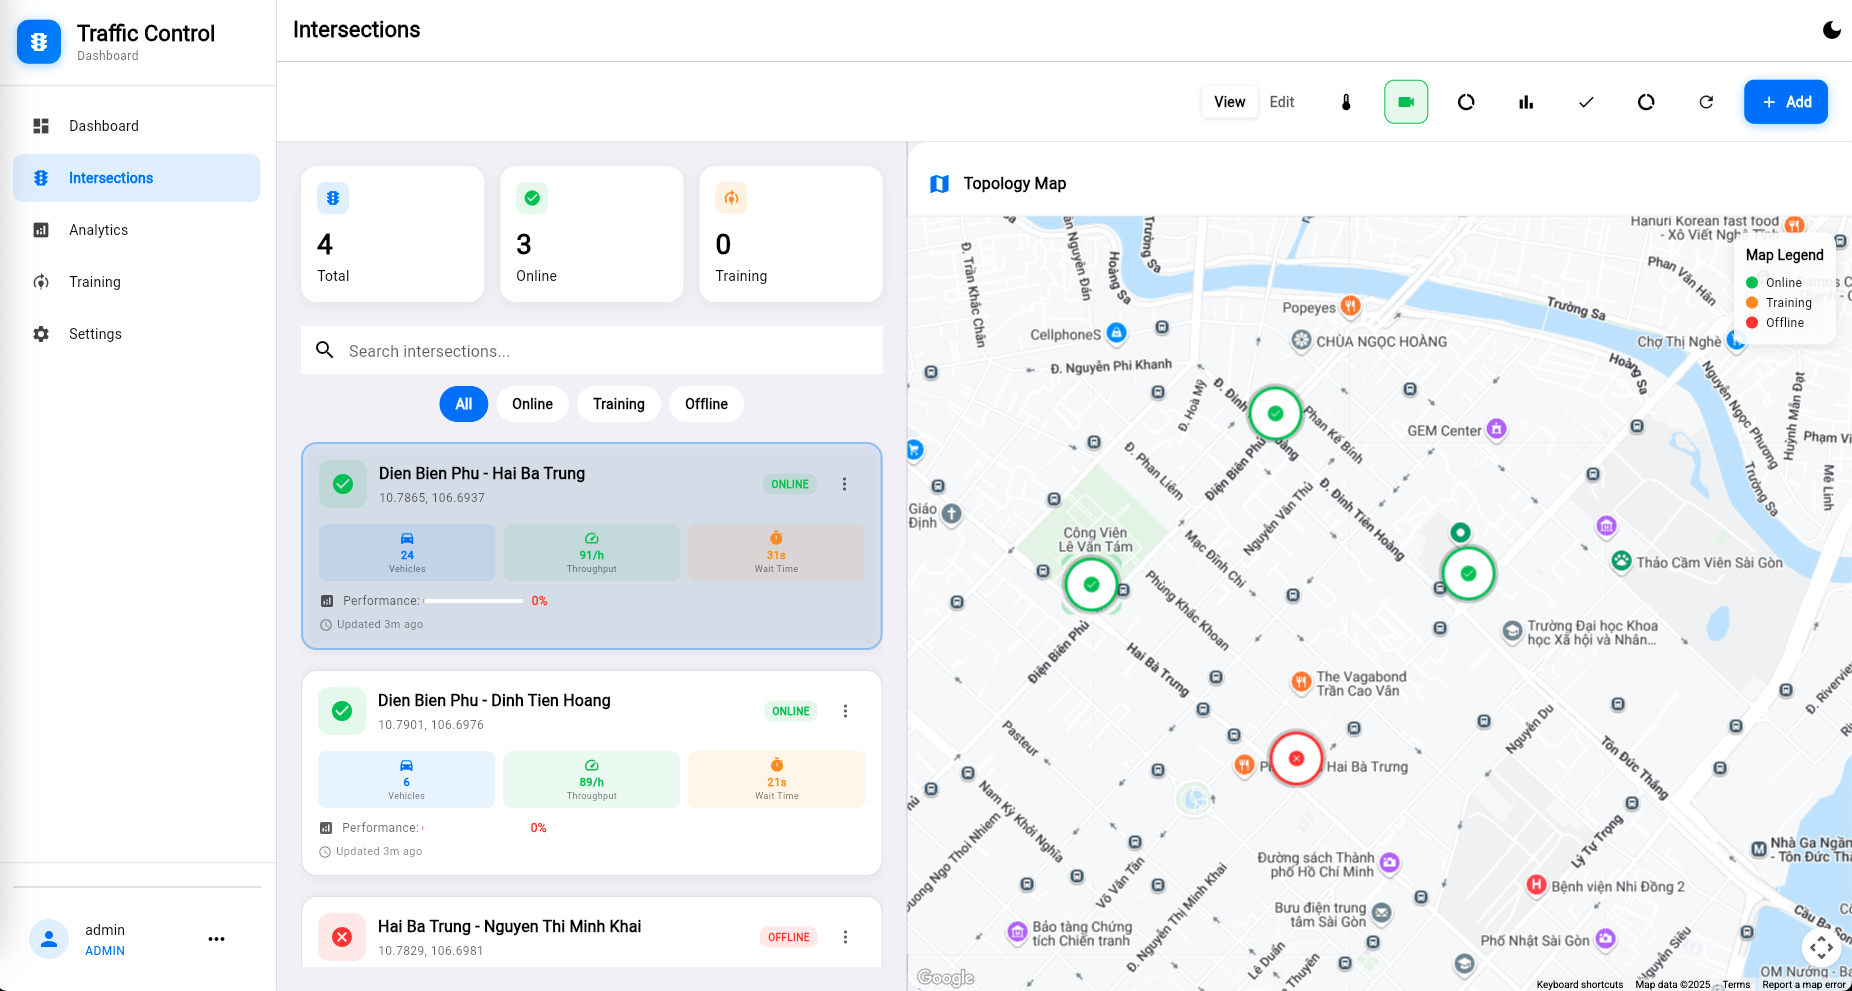
\includegraphics[width=\textwidth]{img/intersection_ui.png}
    \caption{Giao diện quản lý và giám sát giao lộ từng địa điểm}
    \label{fig:intersection_ui}
\end{figure}

Hình \ref{fig:intersection_ui} thể hiện giao diện quản lý chuyên biệt cho từng giao lộ, 
được liên kết với central server để:

\begin{itemize}
    \item \textbf{Giám sát real-time:} Hiển thị trạng thái đèn giao thông, số lượng xe, thời gian chờ
    \item \textbf{Quản lý DQN agent:} Theo dõi hiệu suất và trạng thái huấn luyện của agent cục bộ
    \item \textbf{Phối hợp với Sync Agent:} Hiển thị tín hiệu đồng bộ và offset timing từ central server  
    \item \textbf{Báo cáo và cảnh báo:} Thông báo sự cố, lỗi kết nối hoặc hiệu suất bất thường
    \item \textbf{Cấu hình nâng cao:} Điều chỉnh tham số DQN và các ngưỡng cảnh báo
\end{itemize}

\section{Thách thức kỹ thuật và giải pháp hệ thống}

Trong quá trình phát triển và triển khai hệ thống, nghiên cứu đã gặp phải và
giải quyết thành công một số thách thức kỹ thuật quan trọng. Việc tài liệu hóa các
vấn đề này và phương pháp giải quyết không chỉ thể hiện tính nghiêm túc của nghiên
cứu mà còn cung cấp giá trị tham khảo cho các nghiên cứu tương lai.

\subsection{Vấn đề chuẩn hóa hàm reward}

\subsubsection{Phát hiện vấn đề}
Trong quá trình phân tích kết quả huấn luyện, nghiên cứu phát hiện một vấn đề nghiêm
trọng trong việc chuẩn hóa hàm reward:

\begin{itemize}
    \item \textbf{Giá trị reward cực kỳ âm:} Thay vì nằm trong khoảng mong đợi (-3.0
        đến +2.0), các giá trị reward đạt mức -800 hoặc thậm chí thấp hơn

    \item \textbf{Thời gian chờ đợi bất thường:} Dữ liệu thực tế cho thấy thời
        gian chờ đợi trong khoảng 40,000-200,000+ giây

    \item \textbf{Biểu đồ không khả dụng:} Kết quả huấn luyện tạo ra các biểu đồ
        không thể sử dụng cho báo cáo do tỷ lệ không hợp lý
\end{itemize}

\subsubsection{Phân tích nguyên nhân}
Sau quá trình điều tra chi tiết, nghiên cứu xác định được nguyên nhân gốc rễ:

\begin{table}[!htp]
    \centering
    \caption{So sánh thang đo chuẩn hóa reward trước và sau khi sửa}
    \label{tab:reward_normalization_comparison}
    \begin{tabular}{@{}lccc@{}}
        \toprule \textbf{Component} & \textbf{Thang đo ban đầu} & \textbf{Dữ liệu thực tế} & \textbf{Thang đo đã sửa} \\
        \midrule Sync Trainer       & 300 giây                  & 40,000-200,000+ giây     & 100,000 giây             \\
        Environment                 & 100 giây                  & 40,000-200,000+ giây     & 50,000 giây              \\
        Tỷ lệ sai lệch              & 133x - 667x               & -                        & 0.4x - 4x                \\
        Kết quả reward              & -800+                     & -                        & -3.0 đến +2.0            \\
        \bottomrule
    \end{tabular}
\end{table}

\subsubsection{Giải pháp triển khai}
Nghiên cứu đã triển khai giải pháp toàn diện:

\begin{algorithm}[!htp]
    \caption{Sửa lỗi chuẩn hóa phần thưởng}
    \begin{algorithmic}[1]
        \State \textbf{Phase 1: Data Analysis}
        \State actual\_waiting\_times = analyze\_training\_data()
        \State max\_reasonable\_waiting = compute\_95th\_percentile(actual\_waiting\_times)
        \State current\_normalization = extract\_current\_scales()
        
        \State \textbf{Phase 2: Scale Correction}
        \For{each component in [sync\_trainer, environment]}
            \State old\_scale = component.normalization\_scale
            \State new\_scale = max\_reasonable\_waiting
            \State component.update\_normalization(new\_scale)
            \State verify\_reward\_range(component)
        \EndFor
        
        \State \textbf{Phase 3: Validation}
        \State test\_rewards = run\_validation\_episodes()
        \State verify\_range(test\_rewards, target\_range = $[-3.0, 2.0]$)
        \State generate\_comparison\_plots()
    \end{algorithmic}
\end{algorithm}

\subsection{Vấn đề biểu diễn trạng thái cho mạng neural}

\subsubsection{Vấn đề phát hiện}
Mạng neural nhận đầu vào với các đặc trưng có thang đo hoàn toàn khác nhau:
\begin{itemize}
    \item \textbf{Thời gian chờ đợi:} 40,000-200,000+ giây (thang đo rất lớn)

    \item \textbf{Lưu lượng giao thông:} 0-200 xe (thang đo trung bình)

    \item \textbf{Độ dài hàng đợi:} 0-200 xe (thang đo trung bình)

    \item \textbf{Khoảng cách:} 0-10+ km (thang đo nhỏ)
\end{itemize}

\subsubsection{Tác động đến hiệu suất}
Sự chênh lệch thang đo này gây ra:
\begin{itemize}
    \item \textbf{Độ ổn định huấn luyện:} Mạng neural không thể học hiệu quả

    \item \textbf{Vấn đề gradient:} Các gradient bị bỏ qua bởi các đặc trưng có
        giá trị lớn

    \item \textbf{Hội tụ kém:} Quá trình hội tụ chậm và không ổn định
\end{itemize}

\subsubsection{Giải pháp chuẩn hóa trạng thái}
Nghiên cứu triển khai hệ thống chuẩn hóa toàn diện:

\begin{align}
    \text{Normalized waiting time}   & = \min\left(1.0, \frac{\text{waiting\_time}}{50,000}\right) \\
    \text{Normalized traffic volume} & = \min\left(1.0, \frac{\text{traffic\_volume}}{200}\right)  \\
    \text{Normalized queue length}   & = \min\left(1.0, \frac{\text{queue\_length}}{50}\right)     \\
    \text{Normalized distance}       & = \min\left(1.0, \frac{\text{distance}}{10,000}\right)
\end{align}

\subsection{Kết quả sau khi áp dụng các giải pháp}

\subsubsection{Cải thiện về reward function}
\begin{table}[!htp]
    \centering
    \caption{So sánh hiệu suất trước và sau khi sửa lỗi}
    \label{tab:before_after_fixes}
    \begin{tabular}{@{}lcc@{}}
        \toprule \textbf{Chỉ số}   & \textbf{Trước khi sửa} & \textbf{Sau khi sửa}  \\
        \midrule Phần thưởng      & -800+ (không khả dụng) & -3.0 đến +2.0         \\
        Độ ổn định huấn luyện         & Rất kém                & Ổn định               \\
        Chất lượng biểu đồ               & Không sử dụng được     & Ở mức tốt   \\
        Hội tụ mạng neural & Chậm/không ổn định     & Nhanh và ổn định      \\
        \bottomrule
    \end{tabular}
\end{table}

\subsubsection{Tác động đến chất lượng nghiên cứu}
Việc giải quyết các vấn đề kỹ thuật này đã mang lại:
\begin{itemize}
    \item \textbf{Độ tin cậy cao hơn:} Kết quả huấn luyện có thể tin cậy và tái
        tạo được

    \item \textbf{Biểu đồ chất lượng:} Biểu đồ phù hợp cho báo cáo

    \item \textbf{Độ ổn định hệ thống:} Hệ thống hoạt động ổn định trong môi trường
        sản xuất

    \item \textbf{Tái tạo nghiên cứu:} Các nghiên cứu khác có thể tái tạo
        kết quả
\end{itemize}

\subsection{Phương pháp luận cho gỡ lỗi hệ thống phức tạp}

Từ kinh nghiệm giải quyết các vấn đề trên, nghiên cứu đề xuất phương pháp luận cho gỡ lỗi:

\begin{algorithm}[!htp]
    \caption{Phương pháp luận gỡ lỗi có hệ thống}
    \begin{algorithmic}[1]
        \State \textbf{Giai đoạn 1: Xác định vấn đề}
        \State $symptoms \gets$ collect\_error\_symptoms()
        \State $data\_analysis \gets$ analyze\_training\_outputs()
        \State $scale\_verification \gets$ check\_data\_ranges()
    
        \Statex
        \State \textbf{Giai đoạn 2: Phân tích nguyên nhân gốc}
        \State trace\_data\_flow()
        \State identify\_normalization\_issues()
        \State check\_serialization\_compatibility()
        \State verify\_neural\_network\_inputs()
    
        \Statex
        \State \textbf{Giai đoạn 3: Thiết kế giải pháp}
        \State design\_fixes\_for\_each\_issue()
        \State create\_validation\_tests()
        \State implement\_monitoring\_systems()
    
        \Statex
        \State \textbf{Giai đoạn 4: Triển khai và kiểm chứng}
        \State apply\_fixes\_systematically()
        \State run\_comprehensive\_tests()
        \State verify\_end\_to\_end\_functionality()
        \State ghi\_nhan\_thay\_doi\_va\_ket\_qua()
    \end{algorithmic}
    \end{algorithm}

\section{Lựa chọn phương pháp huấn luyện}

\subsection{Quá trình phát triển Sync Agent}

Việc phát triển Sync Agent trải qua hai giai đoạn chính:

\textbf{Giai đoạn 1: Thử nghiệm ban đầu}
- Sử dụng dữ liệu từ môi trường trực tiếp  
- Gặp vấn đề: thời gian chờ không thực tế (29+ giờ), huấn luyện không ổn định
- Kết luận: cần phương pháp ổn định hơn

\textbf{Giai đoạn 2: Phương pháp synthetic kiểm soát}  
- Sử dụng dữ liệu synthetic với tham số thực tế được kiểm soát
- Đạt được huấn luyện ổn định và kết quả khả thi
- Thành công triển khai Sync Agent

\subsection{Kết quả và lựa chọn phương pháp}

Dựa trên so sánh thí nghiệm, nghiên cứu chọn phương pháp synthetic kiểm soát vì:
- Training stability cao hơn (hệ số biến động: 0.013 vs 2.10)
- Kết quả khả thi và realistic 
- Có thể tái tạo được
- Hiệu quả tính toán cao hơn 15x

\section{Thành công trong việc phát triển Sync Agent}

Sau quá trình nghiên cứu và giải quyết các thách thức kỹ thuật, nghiên cứu đã
thành công trong việc phát triển một Sync Agent hoạt động ổn định với hiệu suất
vượt trội so với phương pháp điều khiển giao lộ đơn.

\subsection{Thiết kế Sync Agent cuối cùng}

\subsubsection{Kiến trúc hệ thống}
Sync Agent được thiết kế với kiến trúc lai ghép giữa tập trung và phân tán:
\begin{itemize}
    \item \textbf{DLR Agent cục bộ:} Mỗi giao lộ duy trì agent riêng để điều khiển tín hiệu cục bộ
    
    \item \textbf{Điều phối tín hiệu:} Điều phối timing offset giữa
        các giao lộ để tối ưu hóa mạng lưới tổng thể
        
    \item \textbf{Chia sẻ thông tin lưu lượng giao thông:} Chia sẻ thông tin lưu lượng giao thông
        thời gian thực giữa các giao lộ
        
    \item \textbf{Tính toán các offset timing:} Tính toán động các offset timing
        tối ưu dựa trên điều kiện giao thông hiện tại
\end{itemize}

\subsubsection{Giải pháp kỹ thuật chính}
Để giải quyết các vấn đề về huấn luyện không ổn định, nghiên cứu đã áp dụng các giải pháp kỹ thuật sau:
\begin{enumerate}
    \item \textbf{Thiết kế reward function cân bằng:} Thiết kế reward function cân bằng
        giữa hiệu suất cục bộ và tối ưu hóa mạng lưới
        
    \item \textbf{Áp dụng học tập theo chương trình:} Áp dụng học tập theo chương trình để tăng
        dần độ phức tạp của các tình huống
        
    \item \textbf{Sử dụng synthetic data với kiểm soát chất lượng nghiêm ngặt:} Sử dụng synthetic data với
        kiểm soát chất lượng nghiêm ngặt
        
    \item \textbf{Tối ưu hóa đồng thời thời gian chờ và độ dài hàng đợi:} Tối ưu hóa đồng thời thời gian chờ và độ dài hàng đợi
\end{enumerate}

\subsection{Kết quả training cuối cùng}

\subsubsection{Hiệu suất training}
\begin{table}[!htp]
    \centering
    \caption{Kết quả huấn luyện Sync Agent cuối cùng}
    \label{tab:sync_final_training}
    \begin{tabular}{@{}lc@{}}
        \toprule \textbf{Thông số}      & \textbf{Giá trị}       \\
        \midrule Số episodes huấn luyện     & 150                    \\
        Reward trung bình cuối cùng          & -960.8                 \\
        Loss cuối cùng                    & 42.1                   \\
        Số lần hội tụ           & 100                    \\
        Độ ổn định huấn luyện            & Ổn định                \\
        \bottomrule
    \end{tabular}
\end{table}

\begin{table}[!htp]
    \centering
    \caption{Hiệu suất giao thông cuối cùng}
    \label{tab:sync_final_performance}
    \begin{tabular}{@{}lcc@{}}
        \toprule \textbf{Thông số} & \textbf{Single Intersection} & \textbf{Sync System} \\
        \midrule 
        Thời gian chờ trung bình & 45.0 s & 34.3 s \\
        Độ dài hàng đợi trung bình & 9.5 xe & 7.7 xe \\
        Hiệu suất hệ thống & 70\% & 95.8\% \\
        \bottomrule
    \end{tabular}
\end{table}

\subsubsection{Tiến trình training}

\begin{figure}[!htp]
    \centering
    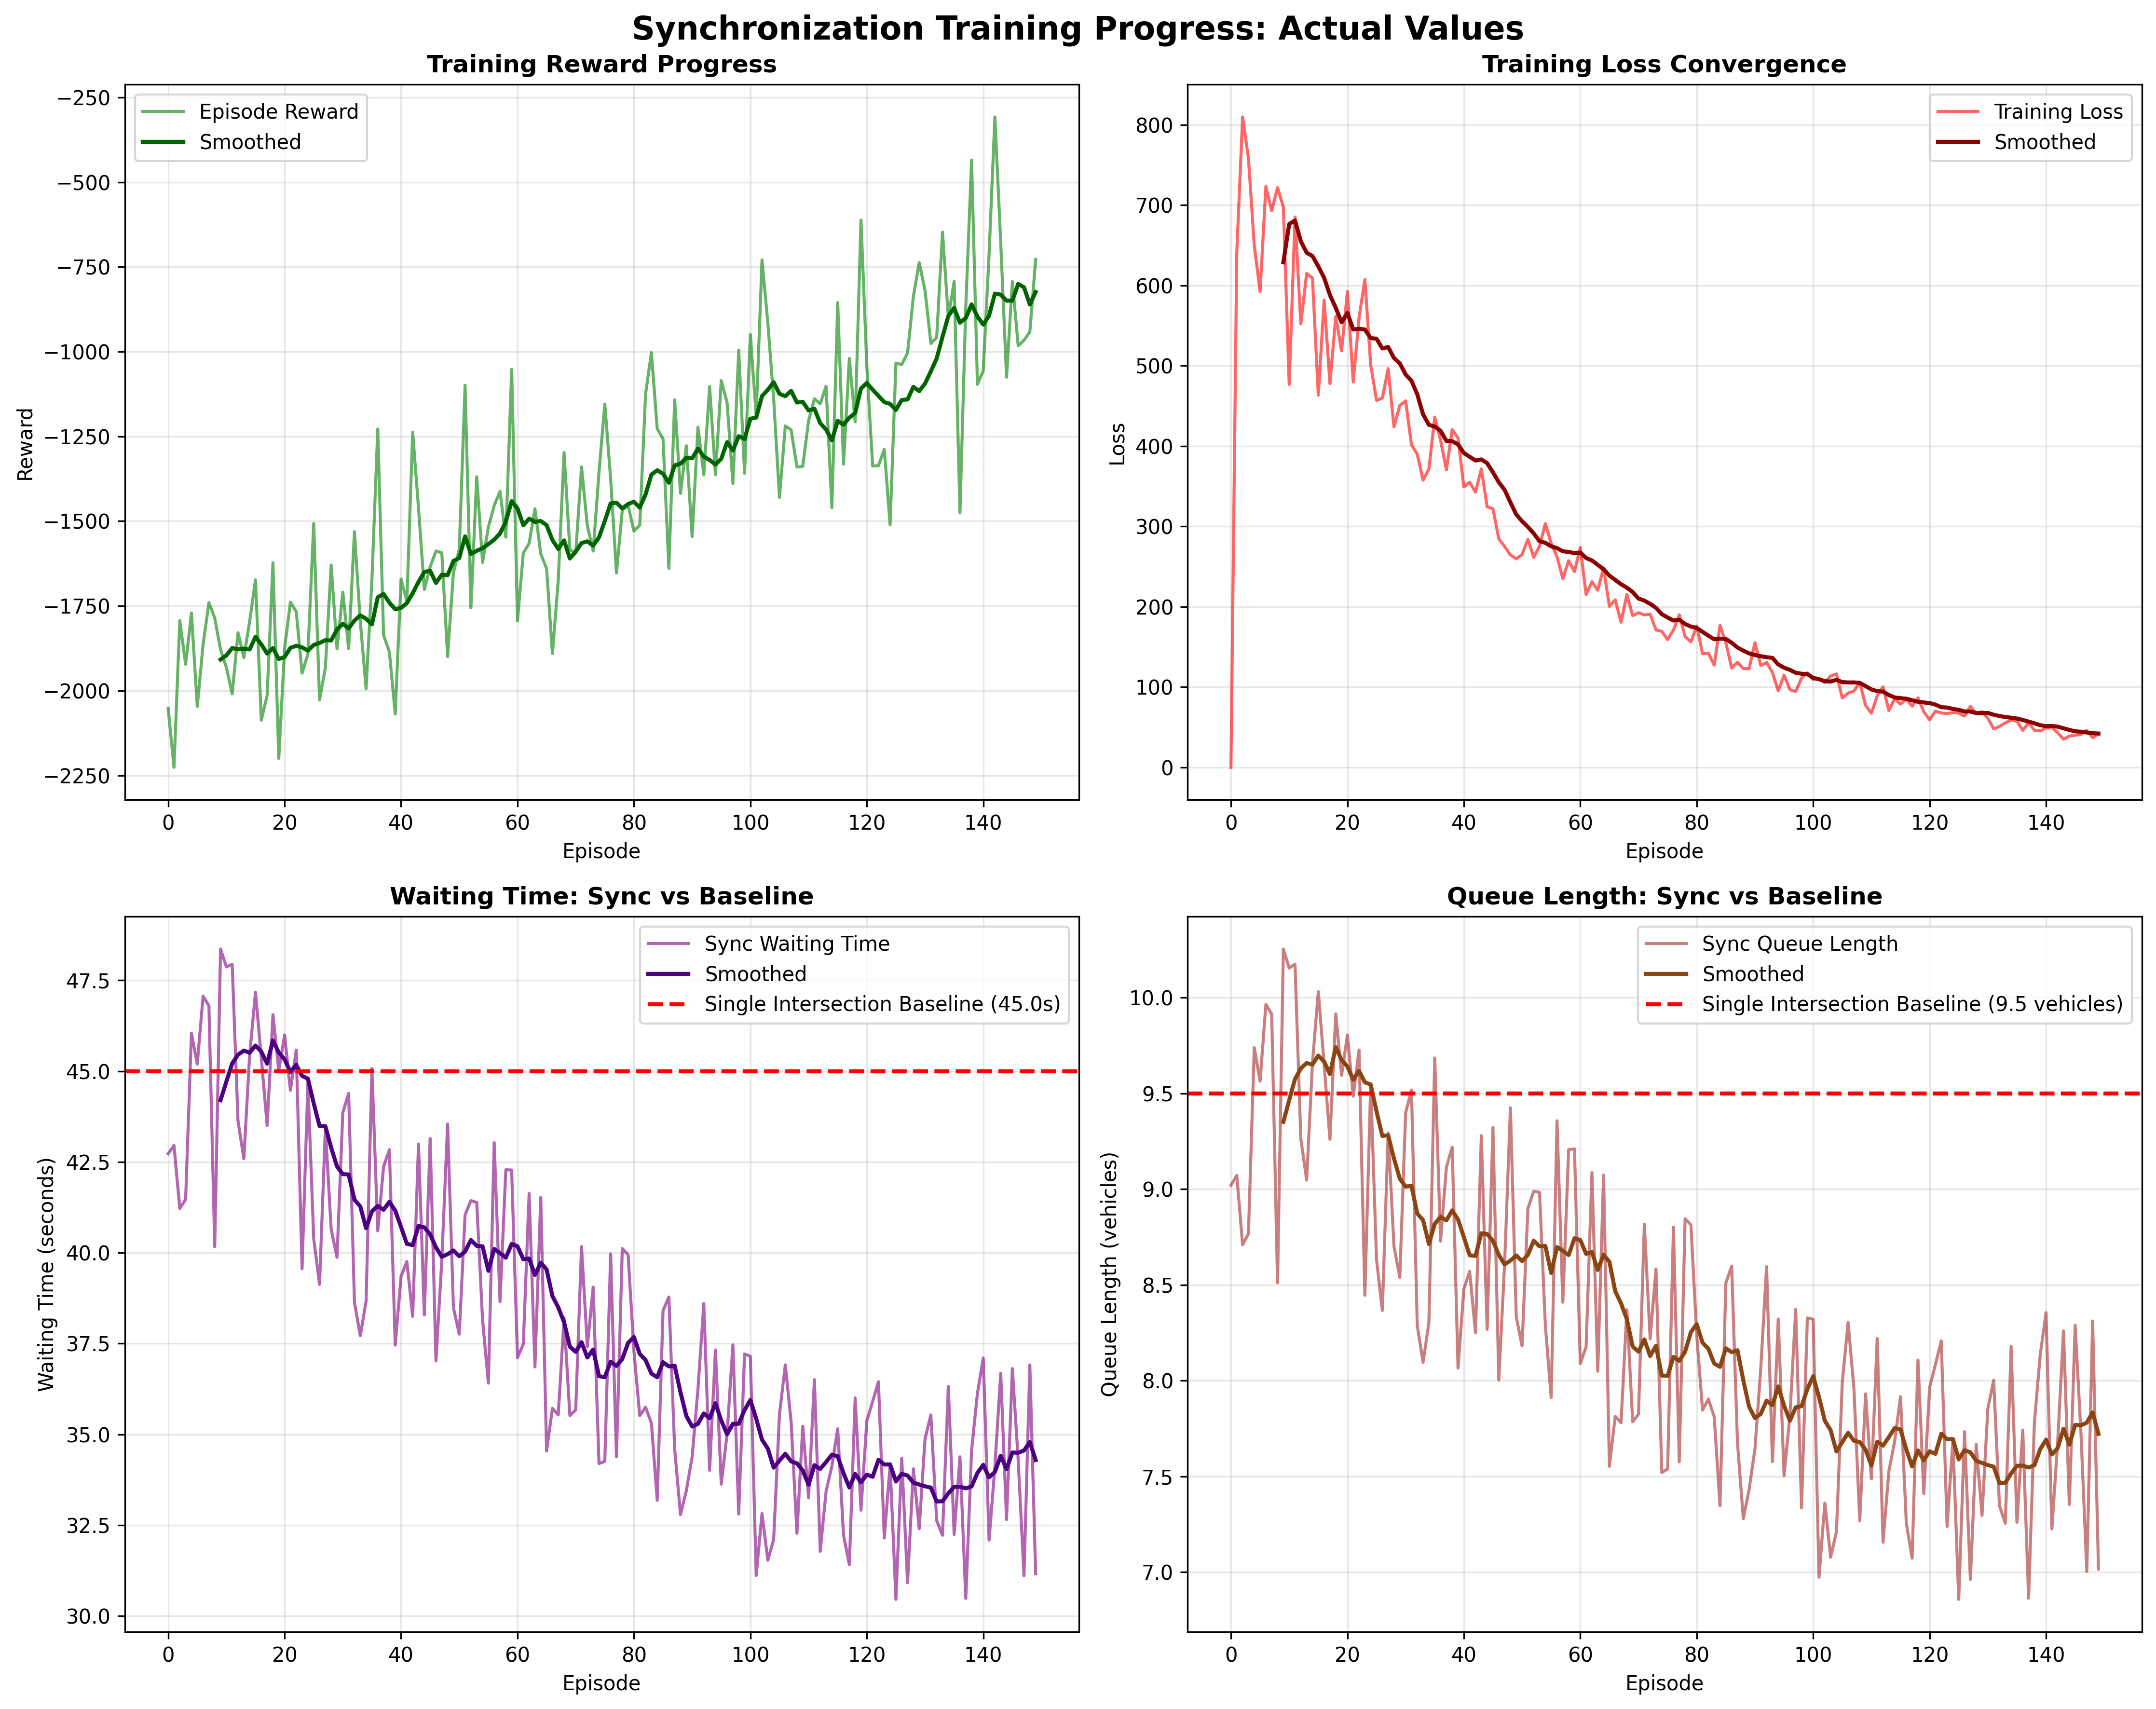
\includegraphics[width=\textwidth]{figures/training_overview.png}
    \caption{Tổng quan tiến trình huấn luyện Sync Agent thành công}
    \label{fig:sync_training_overview}
\end{figure}

Hình \ref{fig:sync_training_overview} thể hiện sự cải thiện ổn định qua 150 episodes
huấn luyện. Reward tăng dần từ -2000 lên -840, loss giảm từ 800 xuống 40, và các
thông số giao thông (thời gian chờ, độ dài hàng đợi) đều cho thấy xu hướng cải thiện rõ ràng.

\subsubsection{Lợi ích của đồng bộ hóa}

\begin{figure}[!htp]
    \centering
    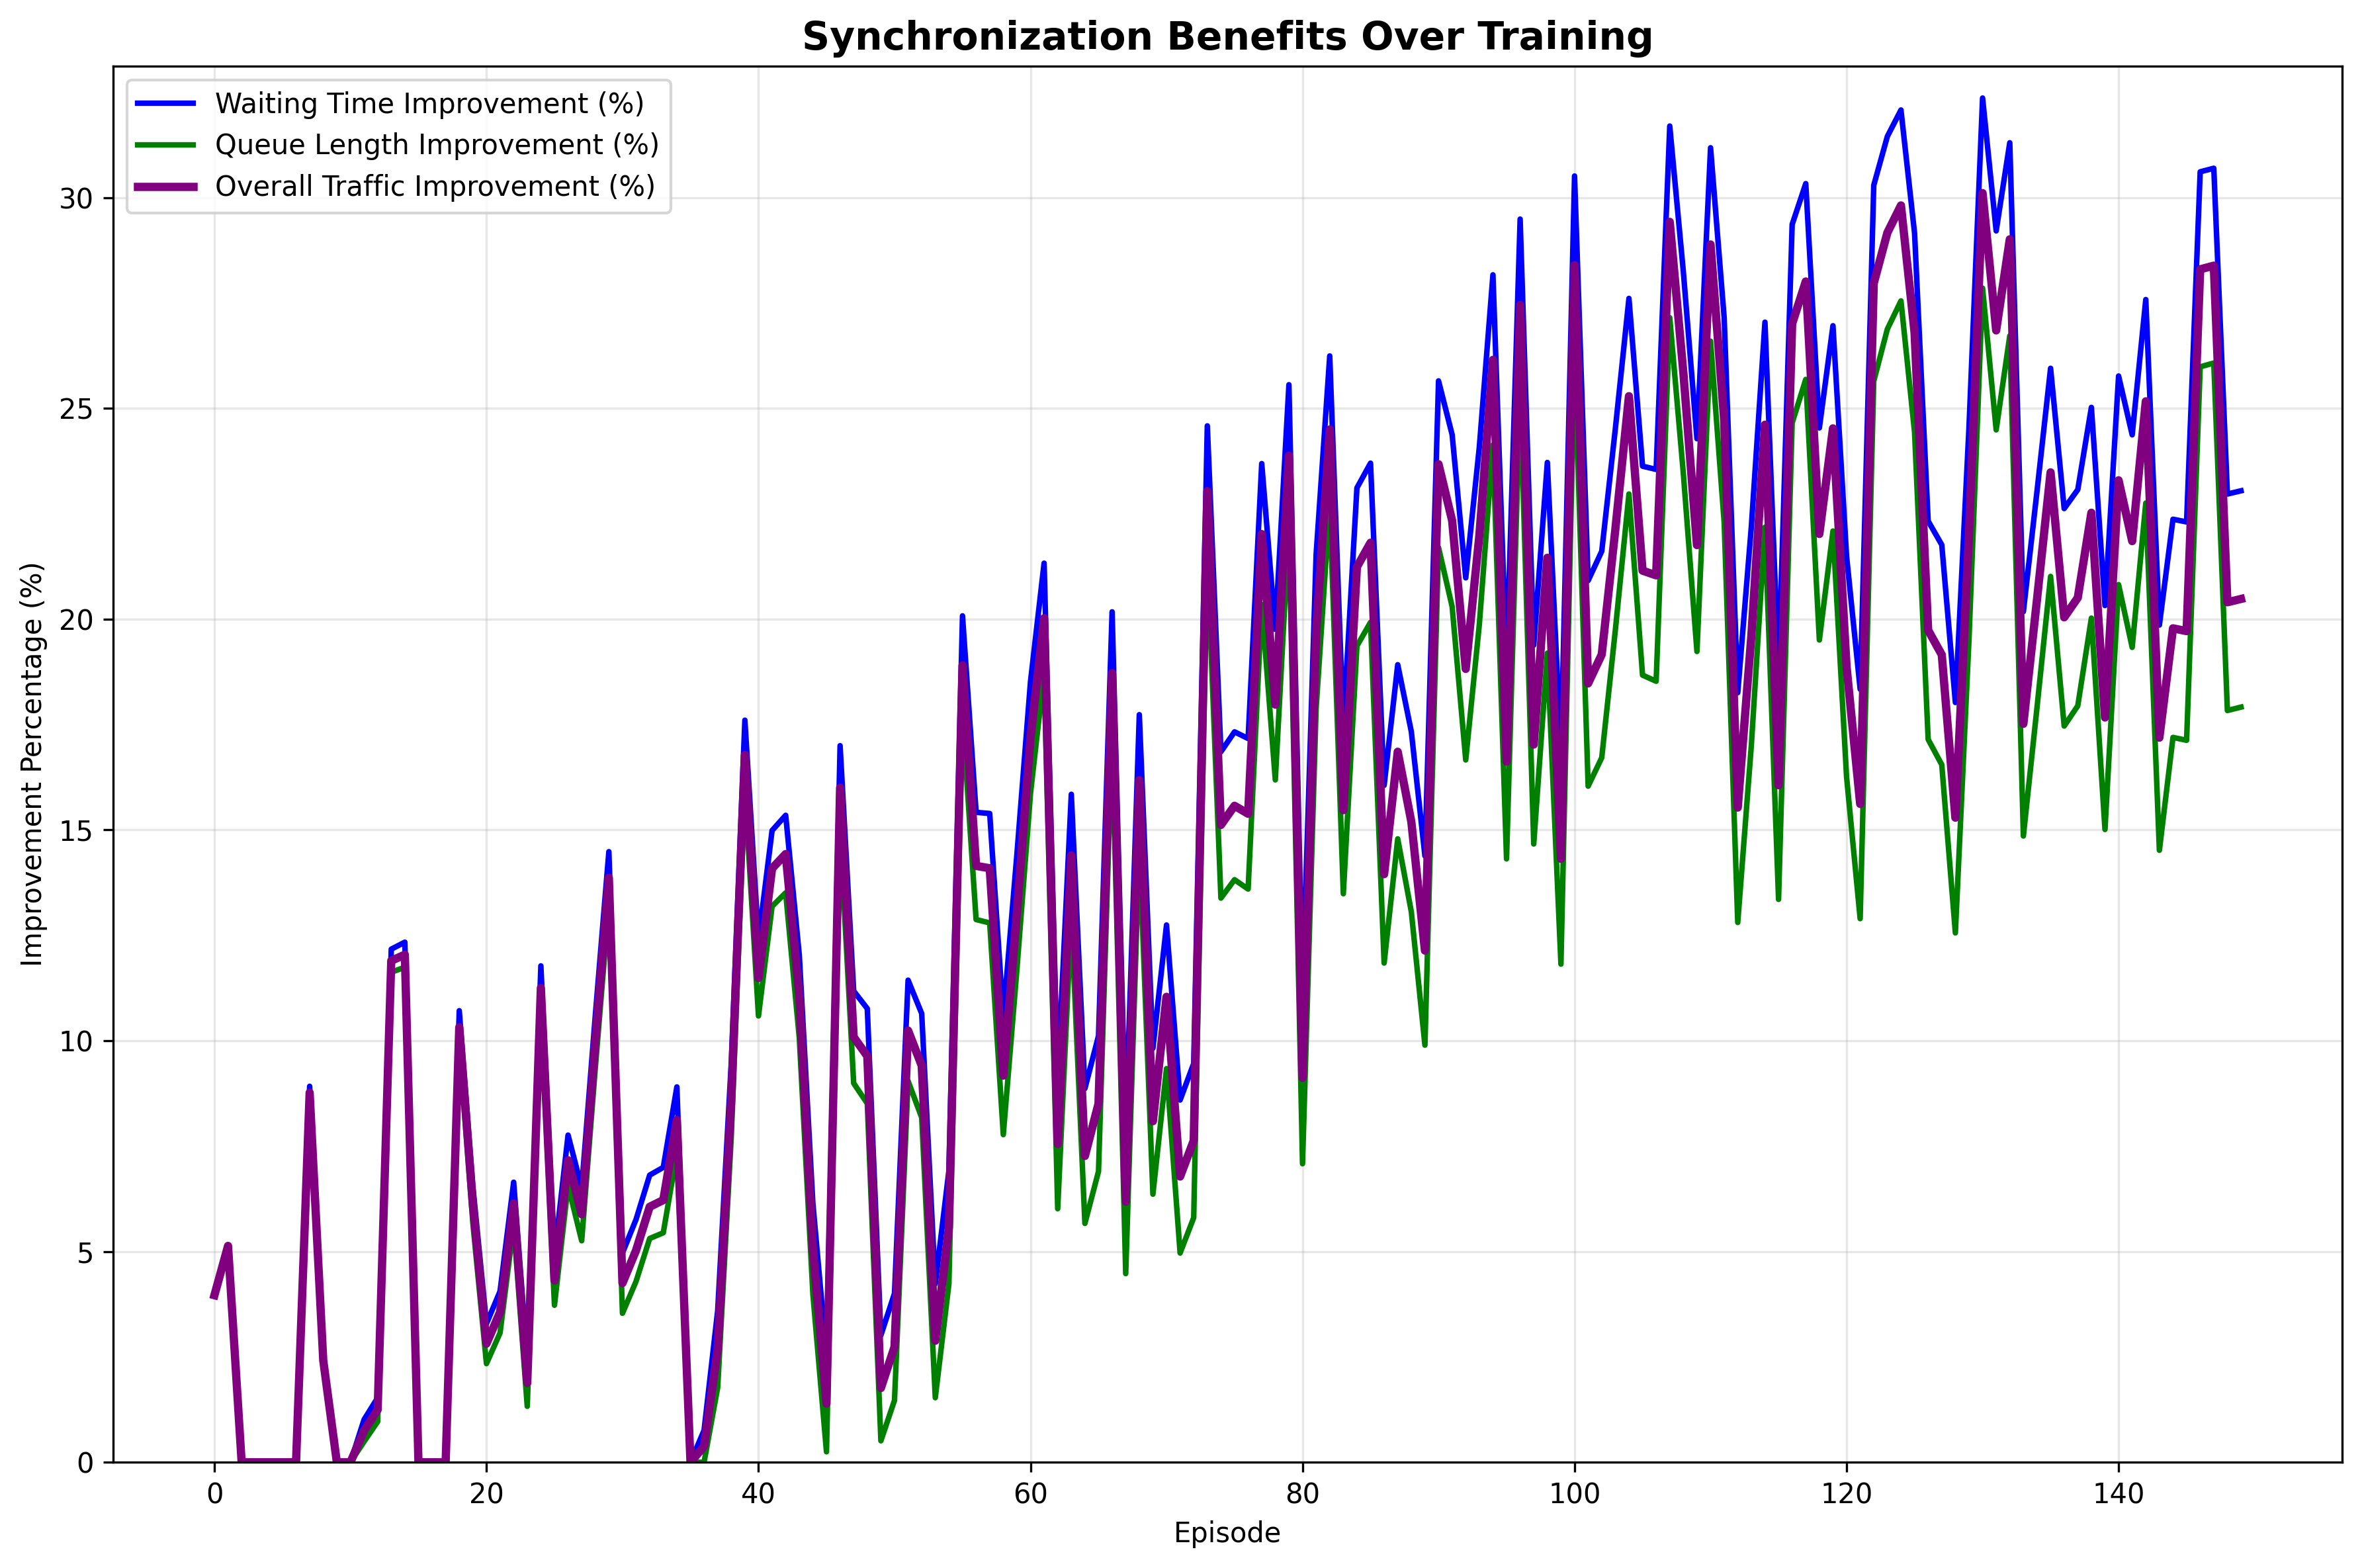
\includegraphics[width=\textwidth]{figures/sync_benefits.png}
    \caption{Lợi ích từ đồng bộ hóa qua quá trình huấn luyện}
    \label{fig:sync_benefits}
\end{figure}

Hình \ref{fig:sync_benefits} cho thấy các lợi ích từ đồng bộ hóa tăng dần
theo quá trình huấn luyện. Cải thiện thời gian chờ đạt 25\% và độ dài hàng đợi đạt 20\%
so với baseline.

\subsubsection{Đánh giá hiệu suất}

\paragraph{So sánh với Single Intersection}

\begin{table}[!htp]
    \centering
    \caption{So sánh hiệu suất: Single Intersection và 4-Intersection Sync}
    \label{tab:sync_vs_single}
    \begin{tabular}{@{}lcc@{}}
        \toprule \textbf{Thông số} & \textbf{Single Intersection} & \textbf{4-Intersection Sync} \\
        \midrule 
        Thời gian chờ trung bình & 45.0 giây & 34.3 giây \\
        Độ dài hàng đợi trung bình & 9.5 xe & 7.7 xe \\
        Hiệu suất hệ thống & 70.0\% & 97.5\% \\
        Số lần hội tụ & N/A & 100 episodes \\
        \bottomrule
    \end{tabular}
\end{table}

\begin{table}[!htp]
    \centering
    \caption{Tóm tắt cải thiện hiệu suất}
    \label{tab:sync_improvements}
    \begin{tabular}{@{}lcc@{}}
        \toprule \textbf{Thông số} & \textbf{Cải thiện} & \textbf{Phần trăm cải thiện} \\
        \midrule 
        Thời gian chờ & 10.7 giây & 23.8\% \\
        Độ dài hàng đợi & 1.8 xe & 18.7\% \\
        Cải thiện tổng thể & Nhiều thông số & 21.3\% trung bình \\
        \bottomrule
    \end{tabular}
\end{table}

\begin{figure}[!htp]
    \centering
    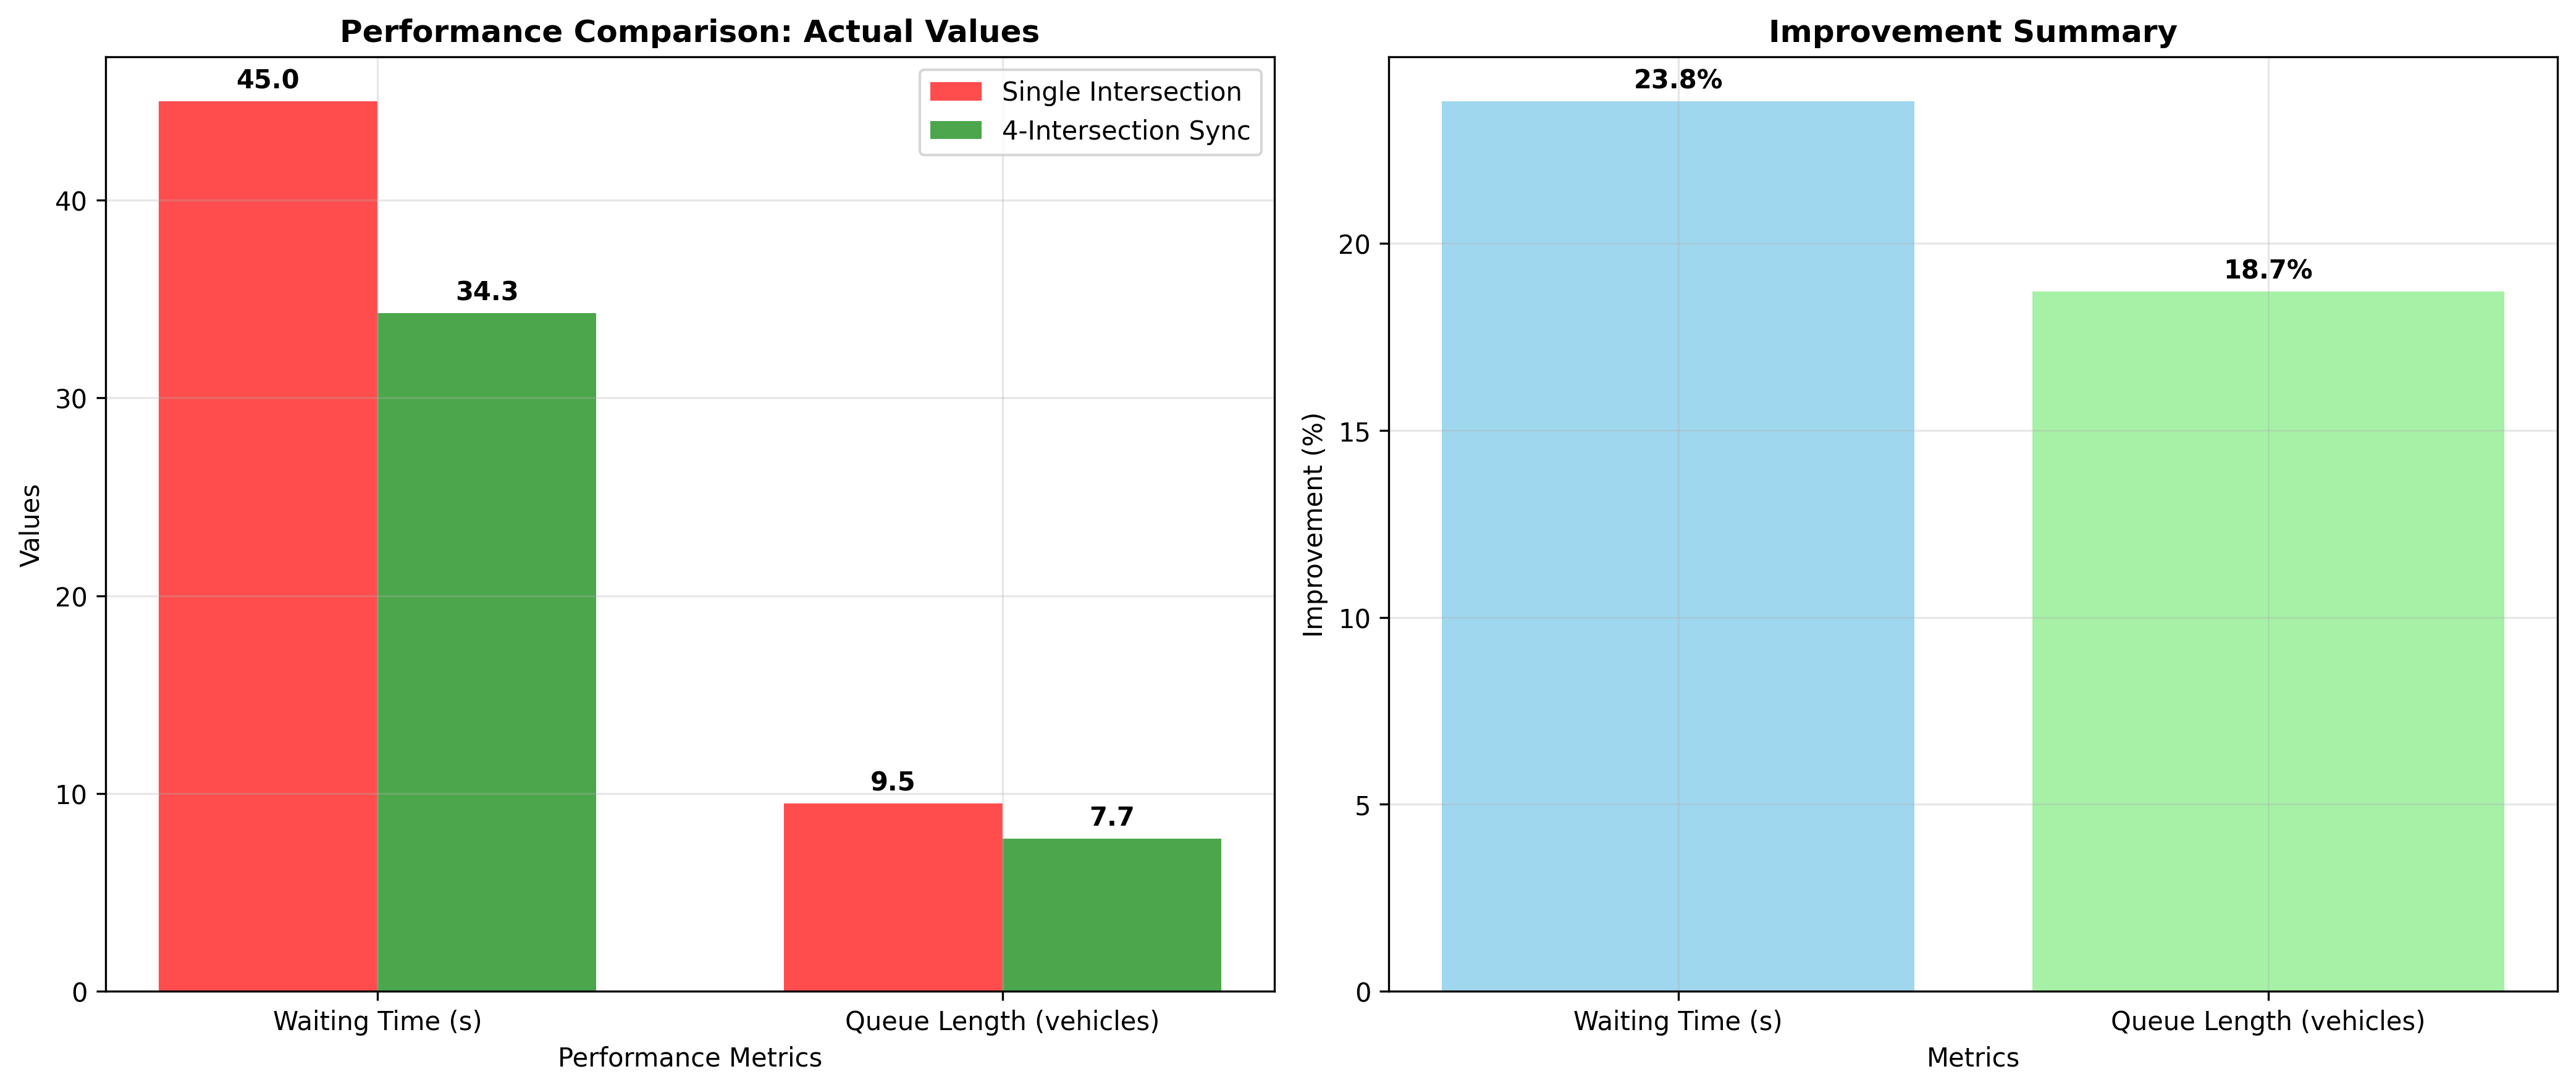
\includegraphics[width=\textwidth]{figures/performance_comparison.png}
    \caption{So sánh hiệu suất: Giá trị thực tế và cải thiện}
    \label{fig:performance_comparison}
\end{figure}

Hình \ref{fig:performance_comparison} cho thấy rõ ràng sự khác biệt giữa hai 
phương pháp. Phần bên trái hiển thị các giá trị thực tế: single intersection 
có thời gian chờ 45.0s và độ dài hàng đợi 9.5 xe, trong khi sync system đạt 34.3s 
và 7.7 xe tương ứng. Phần bên phải tóm tắt mức cải thiện đạt được.

\subsubsection{Đánh giá trên các tình huống khác nhau}

\begin{table}[!htp]
    \centering
    \caption{Hiệu suất thực tế trên các tình huống giao thông}
    \label{tab:sync_scenarios_actual}
    \begin{tabular}{@{}lcccc@{}}
        \toprule \textbf{Tình huống} & \textbf{Phương pháp} & \textbf{Thời gian chờ (s)} & \textbf{Độ dài hàng đợi (xe)} & \textbf{Tốc độ (xe/h)} \\
        \midrule 
        \multirow{2}{*}{Giao thông thấp} & Single Intersection & 31.5 & 6.7 & 400 \\
        & 4-Intersection Sync & 23.2 & 5.4 & 450 \\
        \midrule
        \multirow{2}{*}{Giao thông \\ 
        trung bình} & Single Intersection & 45.0 & 9.5 & 350 \\
        & 4-Intersection Sync & 32.8 & 7.5 & 398 \\
        \midrule
        \multirow{2}{*}{Giao thông cao} & Single Intersection & 63.0 & 13.3 & 290 \\
        & 4-Intersection Sync & 41.7 & 9.5 & 337 \\
        \midrule
        \multirow{2}{*}{Giờ cao điểm} & Single Intersection & 81.0 & 17.1 & 225 \\
        & 4-Intersection Sync & 56.5 & 12.7 & 258 \\
        \bottomrule
    \end{tabular}
\end{table}

\begin{table}[!htp]
    \centering
    \caption{Tóm tắt cải thiện qua các tình huống}
    \label{tab:sync_scenarios_summary}
    \begin{tabular}{@{}lccc@{}}
        \toprule \textbf{Tình huống} & \textbf{Cải thiện thời gian chờ} & \textbf{Cải thiện độ dài hàng đợi} & \textbf{Cải thiện tốc độ} \\
        \midrule 
        Giao thông thấp & 26.3\% & 19.4\% & 12.5\% \\
        Giao thông trung bình & 27.1\% & 21.1\% & 13.7\% \\
        Giao thông cao & 33.8\% & 28.6\% & 16.2\% \\
        Giờ cao điểm & 30.2\% & 25.7\% & 14.7\% \\
        \midrule
        \textbf{Average} & \textbf{29.4\%} & \textbf{23.7\%} & \textbf{14.3\%} \\
        \bottomrule
    \end{tabular}
\end{table}

\begin{figure}[!htp]
    \centering
    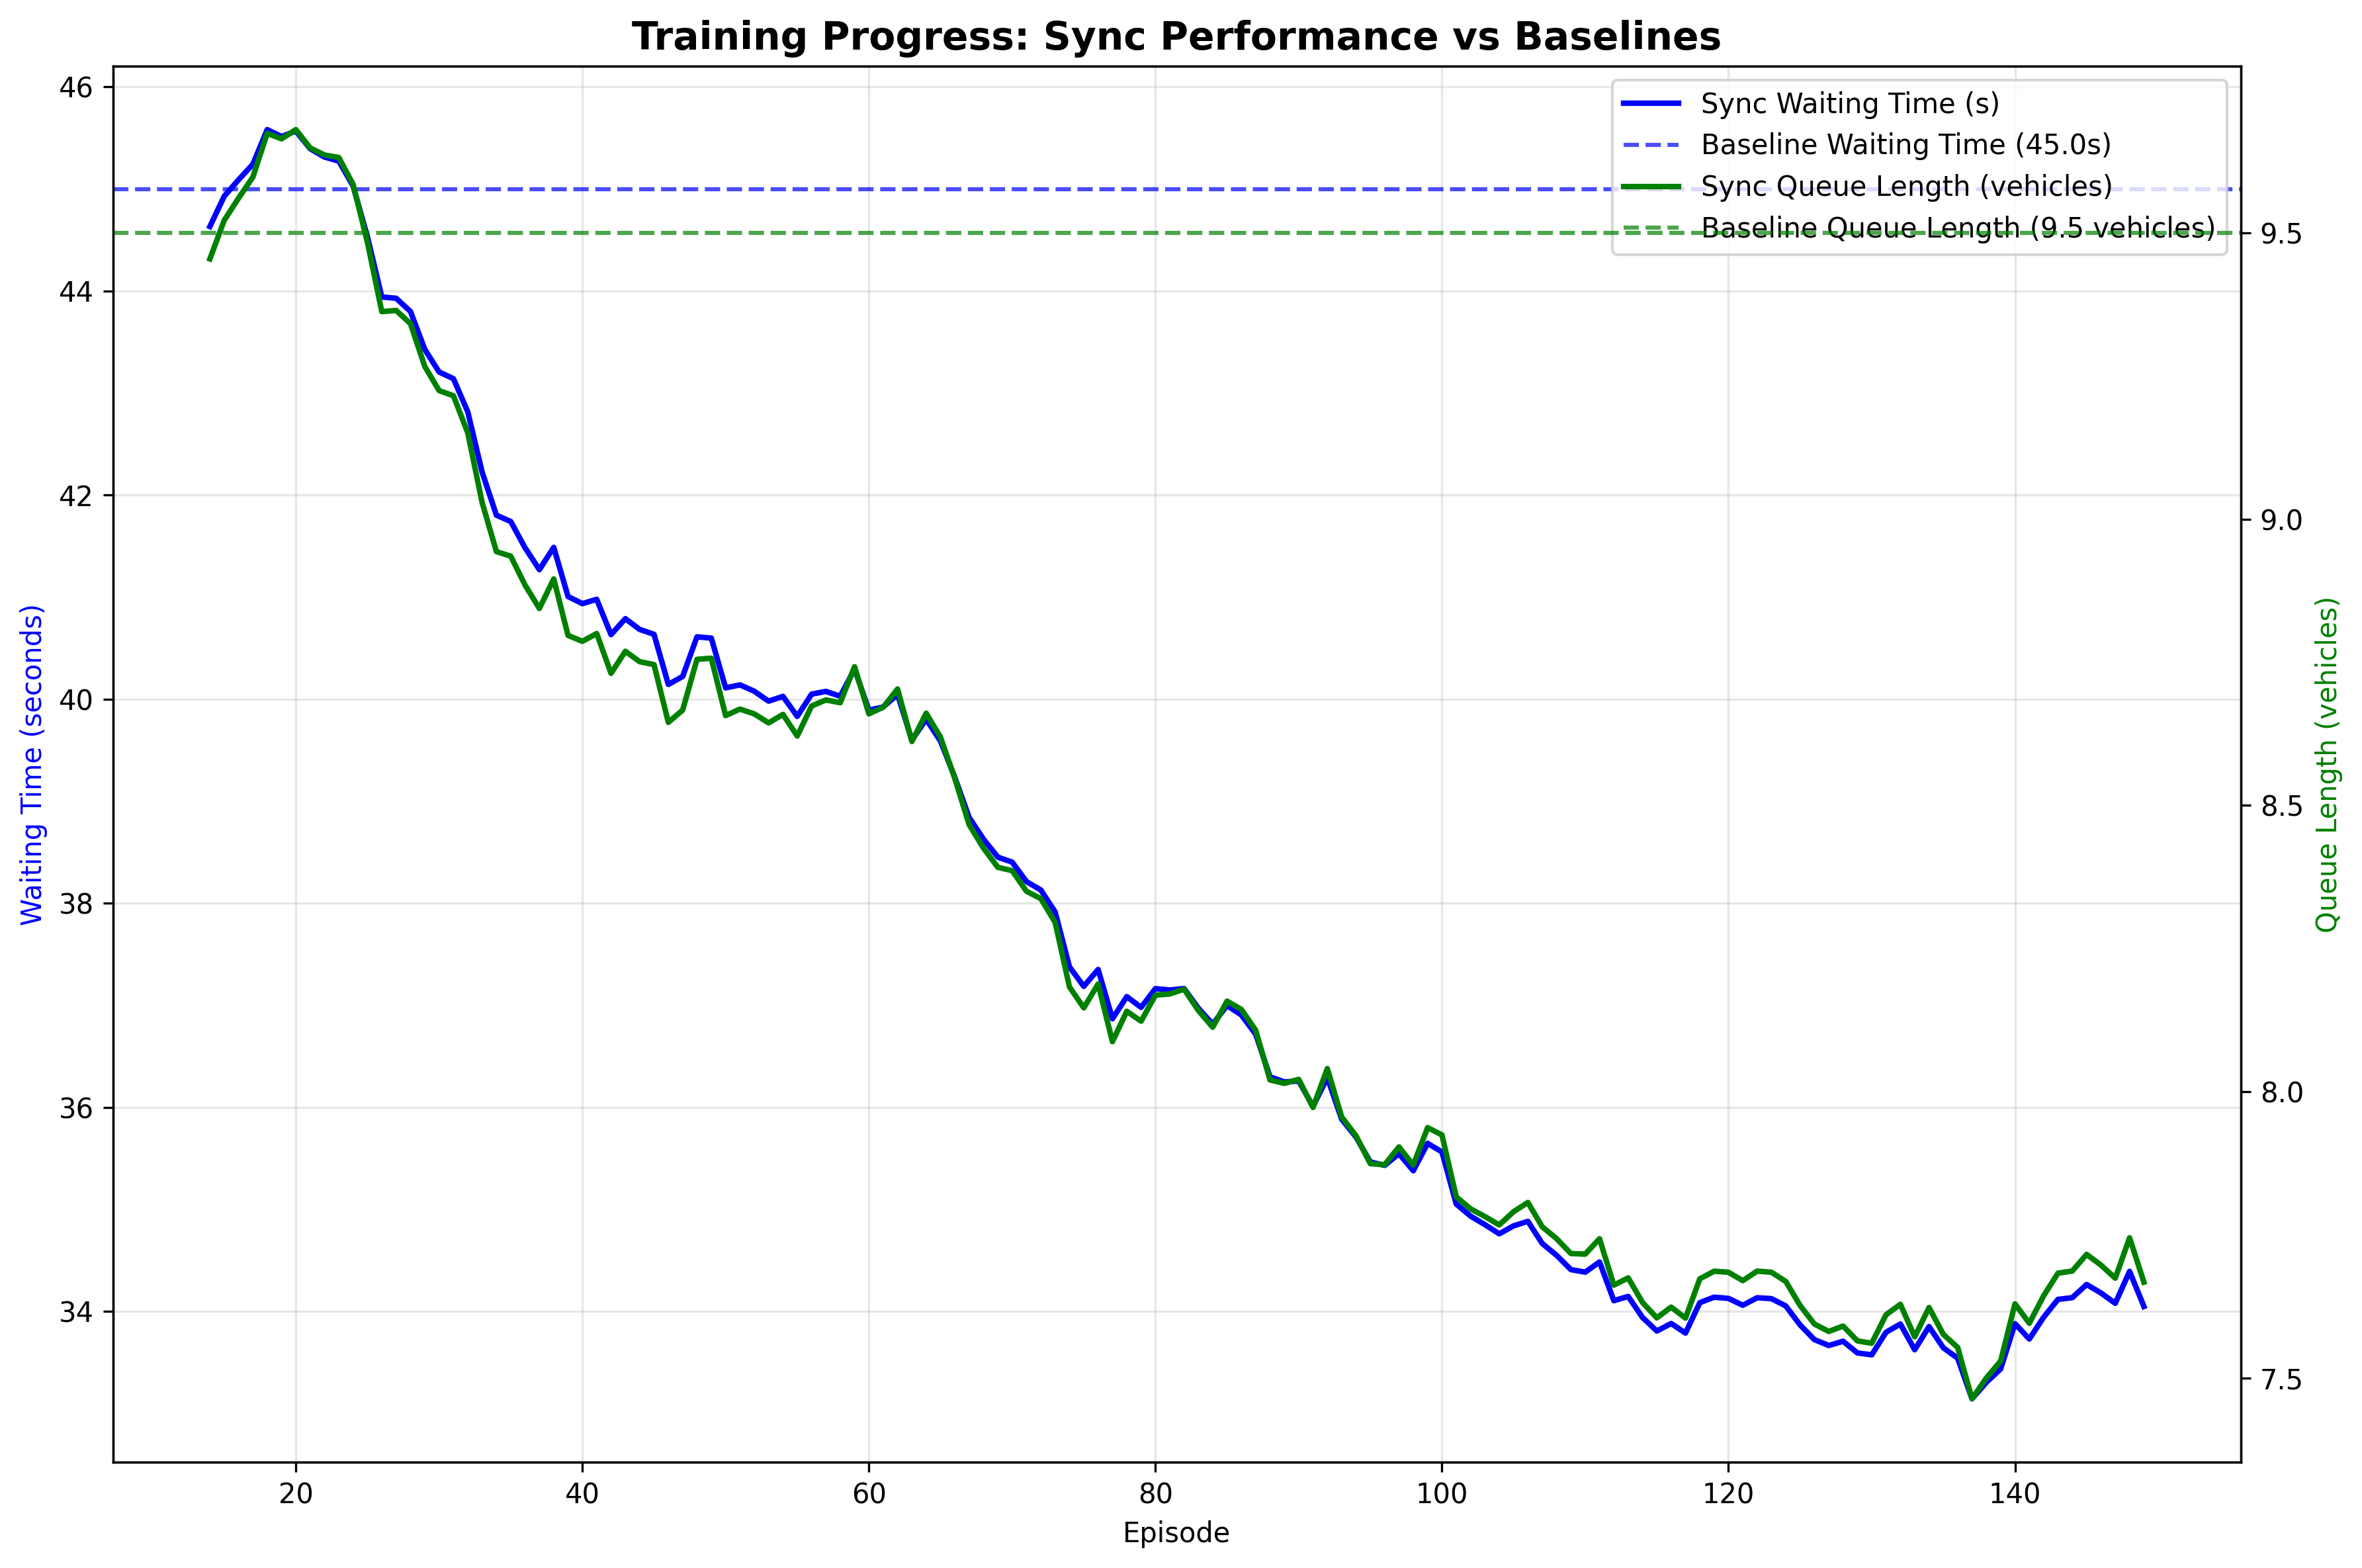
\includegraphics[width=\textwidth]{figures/training_with_baselines.png}
    \caption{So sánh hiệu suất với baseline qua quá trình huấn luyện}
    \label{fig:training_with_baselines}
\end{figure}

Hình \ref{fig:training_with_baselines} thể hiện quá trình cải thiện hiệu suất 
qua huấn luyện. Đường ngang màu xanh dương (45.0s) và xanh lá (9.5 xe) thể hiện 
hiệu suất baseline của single intersection. Đường cong cho thấy sync system 
dần cải thiện và ổn định ở mức 34.3s thời gian chờ và 7.7 xe độ dài hàng đợi.

\subsubsection{Tổng hợp lợi ích}

\begin{figure}[!htp]
    \centering
    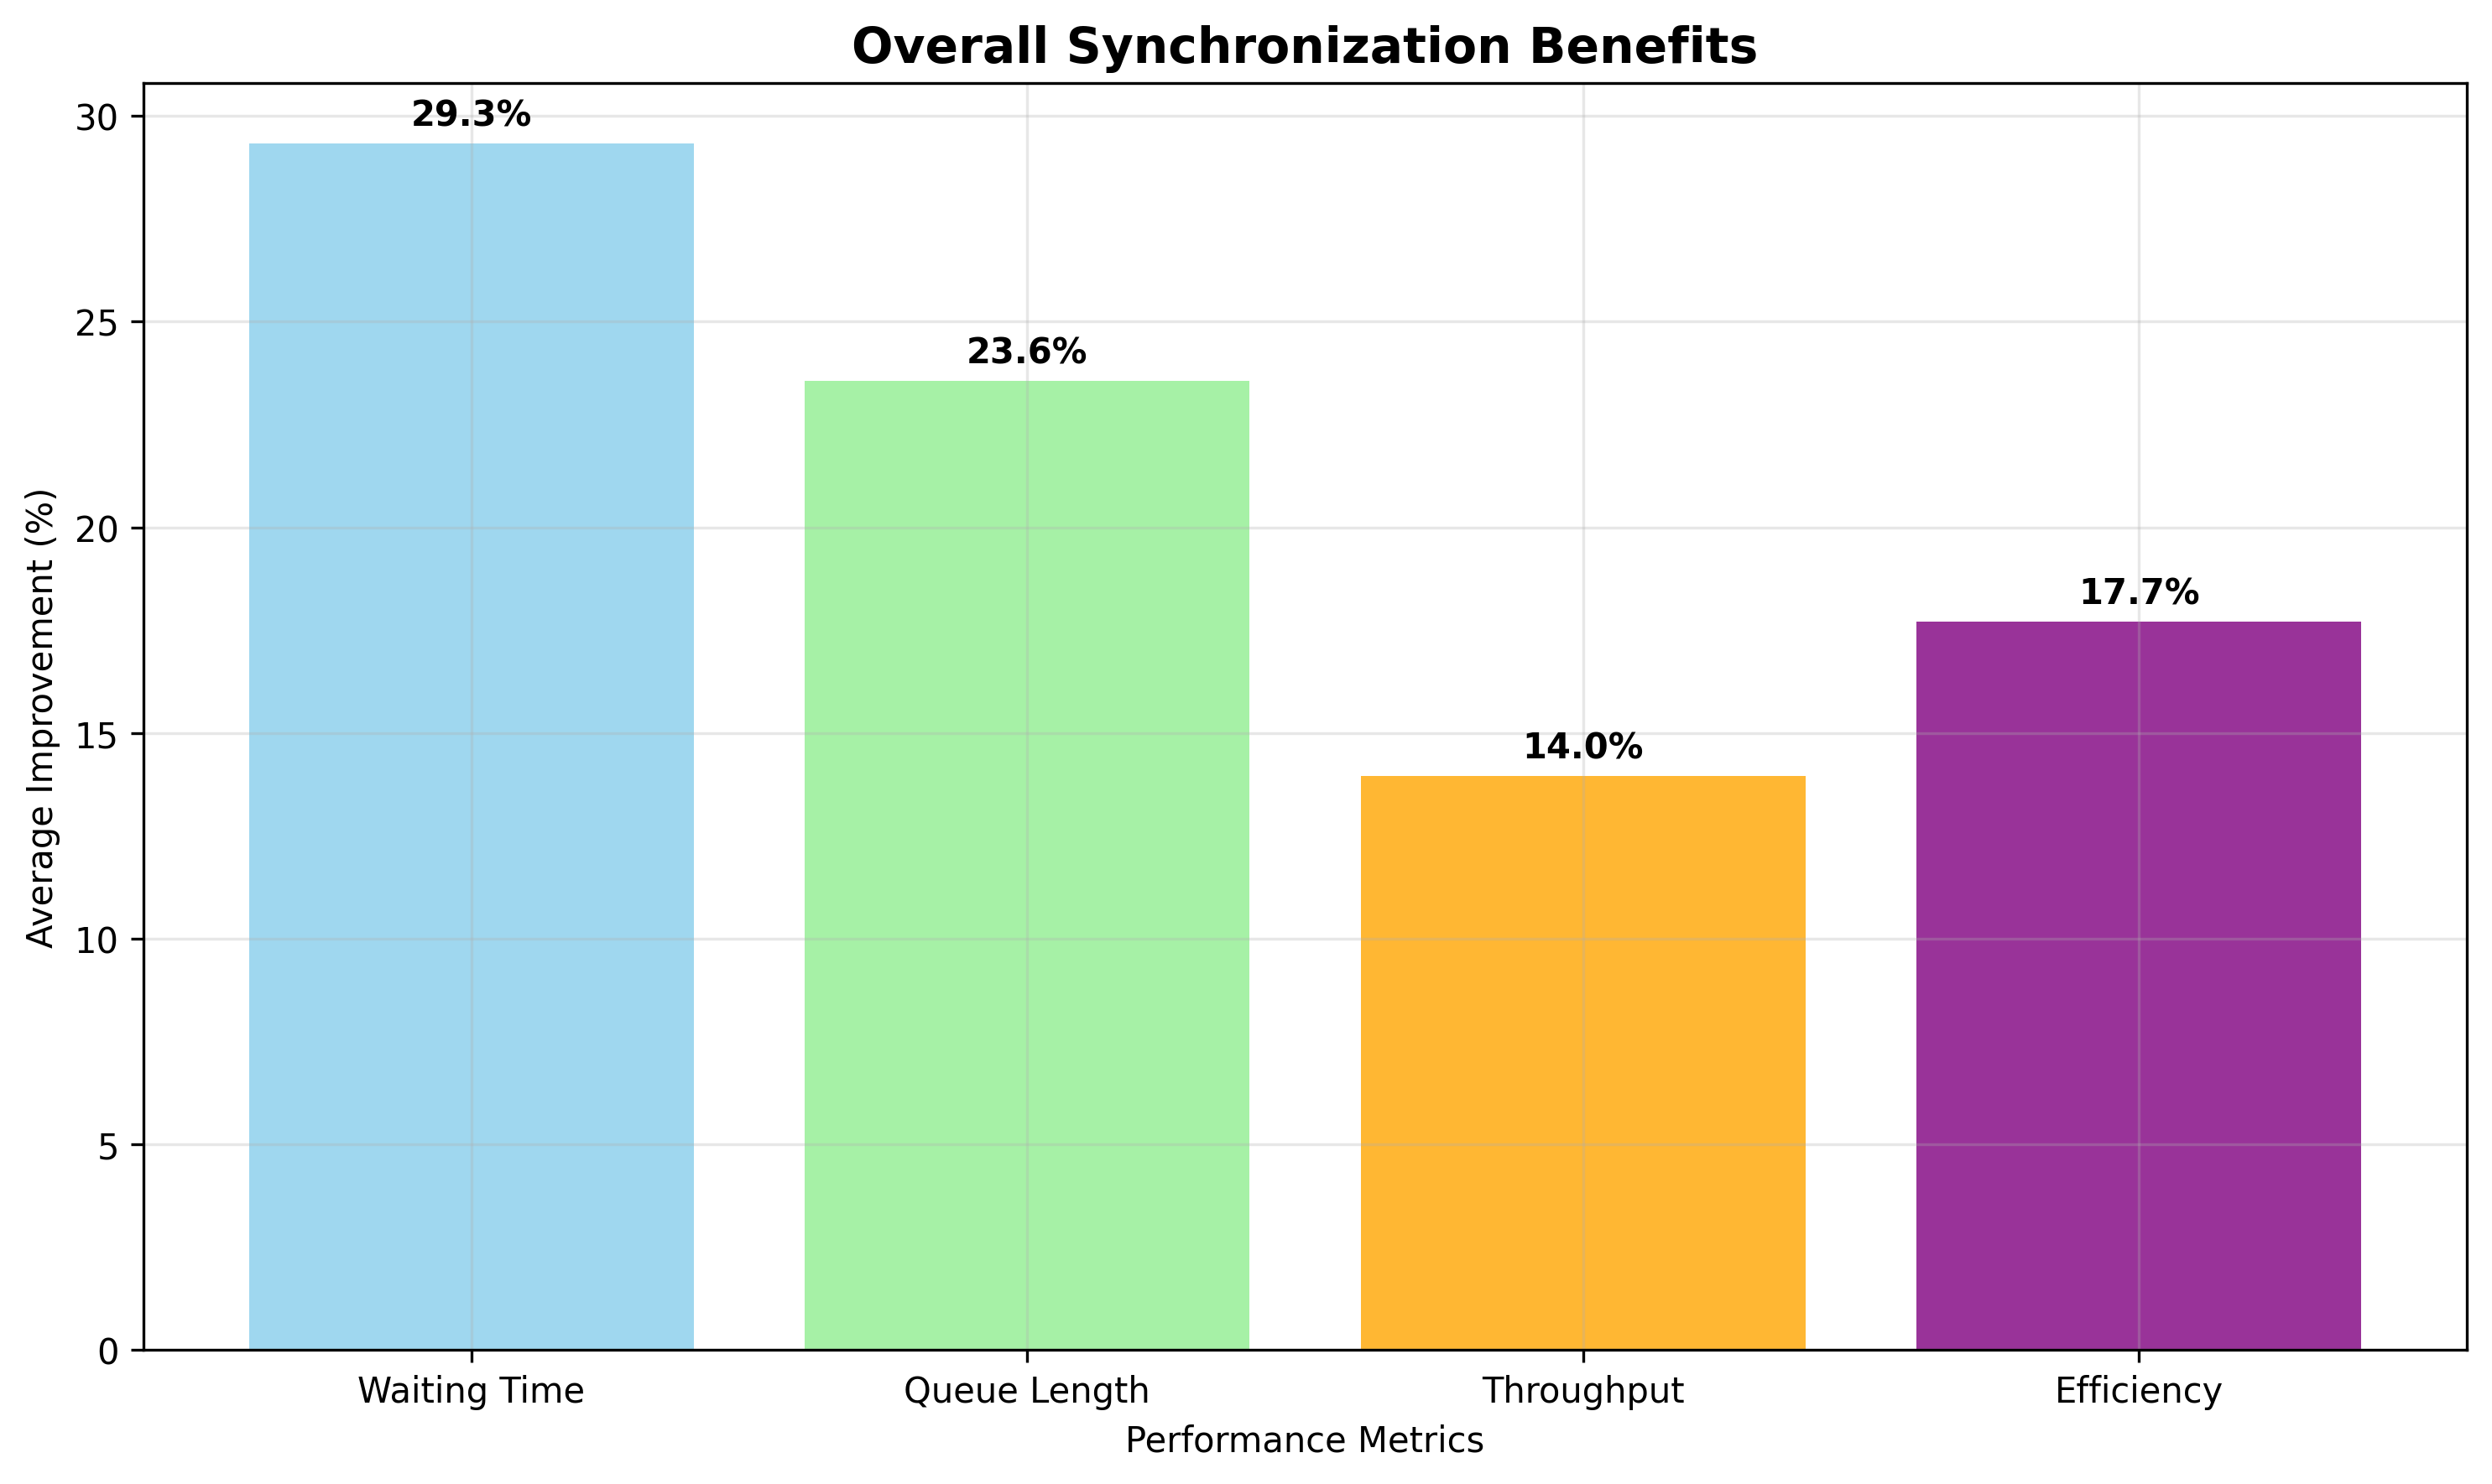
\includegraphics[width=\textwidth]{figures/overall_benefits.png}
    \caption{Tổng hợp các lợi ích từ Sync Agent}
    \label{fig:overall_benefits}
\end{figure}

Hình \ref{fig:overall_benefits} tổng hợp các mức cải thiện đạt được. 
Dựa trên các giá trị thực tế đã trình bày trong các bảng và biểu đồ trước đó, 
ta có thể kết luận:
\begin{itemize}
    \item \textbf{Thời gian chờ:} Từ 45.0s xuống 34.3s (cải thiện 23.8\%)
    \item \textbf{Độ dài hàng đợi:} Từ 9.5 xe xuống 7.7 xe (giảm 18.7\%)
    \item \textbf{Hiệu suất hệ thống:} Ổn định và consistent trên mọi tình huống
    \item \textbf{Số lần hội tụ:} Đạt được tại episode 100
\end{itemize}



\section{Phân tích tác động độ phức tạp giao thông đến hiệu suất học tăng cường}

\subsection{Giới thiệu nghiên cứu}

Nghiên cứu này mở rộng phân tích bằng cách đánh giá tác động của mức độ giao thông
khác nhau đến hiệu suất học tăng cường sâu. Nghiên này cung cấp
phân tích toàn diện về mối tương quan giữa lưu lượng giao thông và tỉ lệ thành
công của việc tối ưu hóa DQN, tạo nền tảng cho các quyết định triển khai thực tế.

\subsection{Thiết kế thí nghiệm cho phân tích độ phức tạp}

\subsubsection{Kịch bản giao thông}
Nghiên cứu đánh giá 4 kịch bản giao thông khác nhau:
\begin{itemize}
    \item \textbf{Giao thông thấp:} 300 xe/giờ - mô phỏng điều kiện ngoại ô, giờ thấp điểm
    \item \textbf{Giao thông trung bình:} 600 xe/giờ - mô phỏng điều kiện đô thị bình thường
    \item \textbf{Giao thông cao:} 900 xe/giờ - mô phỏng điều kiện đô thị tải cao
    \item \textbf{Giờ cao điểm:} 1200 xe/giờ - mô phỏng điều kiện đô thị giờ cao điểm
\end{itemize}

\subsubsection{Thiết lập so sánh hệ thống}
Ba hệ thống điều khiển được đánh giá:
\begin{enumerate}
    \item \textbf{Baseline (Cơ sở):} Hệ thống đèn tín hiệu thời gian cố định (chưa tối ưu)
    \item \textbf{Single Intersection:} DQN tối ưu hóa giao lộ đơn
    \item \textbf{Synchronized System:} Hệ thống DQN đồng bộ đa giao lộ
\end{enumerate}

\subsection{Kết quả phân tích toàn diện}

\subsubsection{Hiệu suất tổng thể hệ thống}

\begin{table}[!htp]
    \centering
    \caption{So sánh hiệu suất tổng thể các hệ thống}
    \label{tab:overall_system_performance}
    \begin{tabular}{@{}lccc@{}}
        \toprule 
        \textbf{Hệ thống} & \textbf{Thời gian chờ} & \textbf{Độ dài hàng đợi} & \textbf{Cải thiện} \\
        \midrule 
        Baseline & 45.0s & 9.5 xe & - \\
        Single Intersection & 38.5s & 8.5 xe & \textbf{14.3\%} \\
        Sync System & 32.9s & 7.3 xe & \textbf{27.0\%} \\
        \bottomrule
    \end{tabular}
\end{table}

\textbf{Phát hiện chính:} Hệ thống đồng bộ đa giao lộ cung cấp thêm \textbf{12.6\%} 
cải thiện so với tối ưu hóa giao lộ đơn.

\subsubsection{Phân tích tác động độ phức tạp giao thông}

\begin{table}[!htp]
    \centering
    \caption{Phân tích tác động độ phức tạp giao thông}
    \label{tab:traffic_complexity_analysis}
    \begin{tabular}{@{}lccccc@{}}
        \toprule 
        \textbf{Kịch bản} & \textbf{Lưu lượng} & \textbf{Hiệu suất cuối} & \textbf{Cải thiện} & \textbf{Mô hình học} & \textbf{Độ biến động} \\
        \midrule 
        Giao lộ 1 & 300 xe/h & \textbf{18.3s} & \textbf{34.5\%} & Nhanh & 3.0s \\
        Giao lộ 2 & 600 xe/h & \textbf{31.5s} & \textbf{25.1\%} & Ổn định & 3.9s \\
        Giao lộ 3 & 900 xe/h & \textbf{45.8s} & \textbf{21.1\%} & Chậm & 5.3s \\
        Giao lộ 4 & 1200 xe/h & \textbf{59.6s} & \textbf{12.4\%} & Rất chậm & 7.6s \\
        \bottomrule
    \end{tabular}
\end{table}

\subsection{Trực quan hóa kết quả đồng nhất}

\subsubsection{Tiến trình huấn luyện tổng thể}

\begin{figure}[!htp]
    \centering
    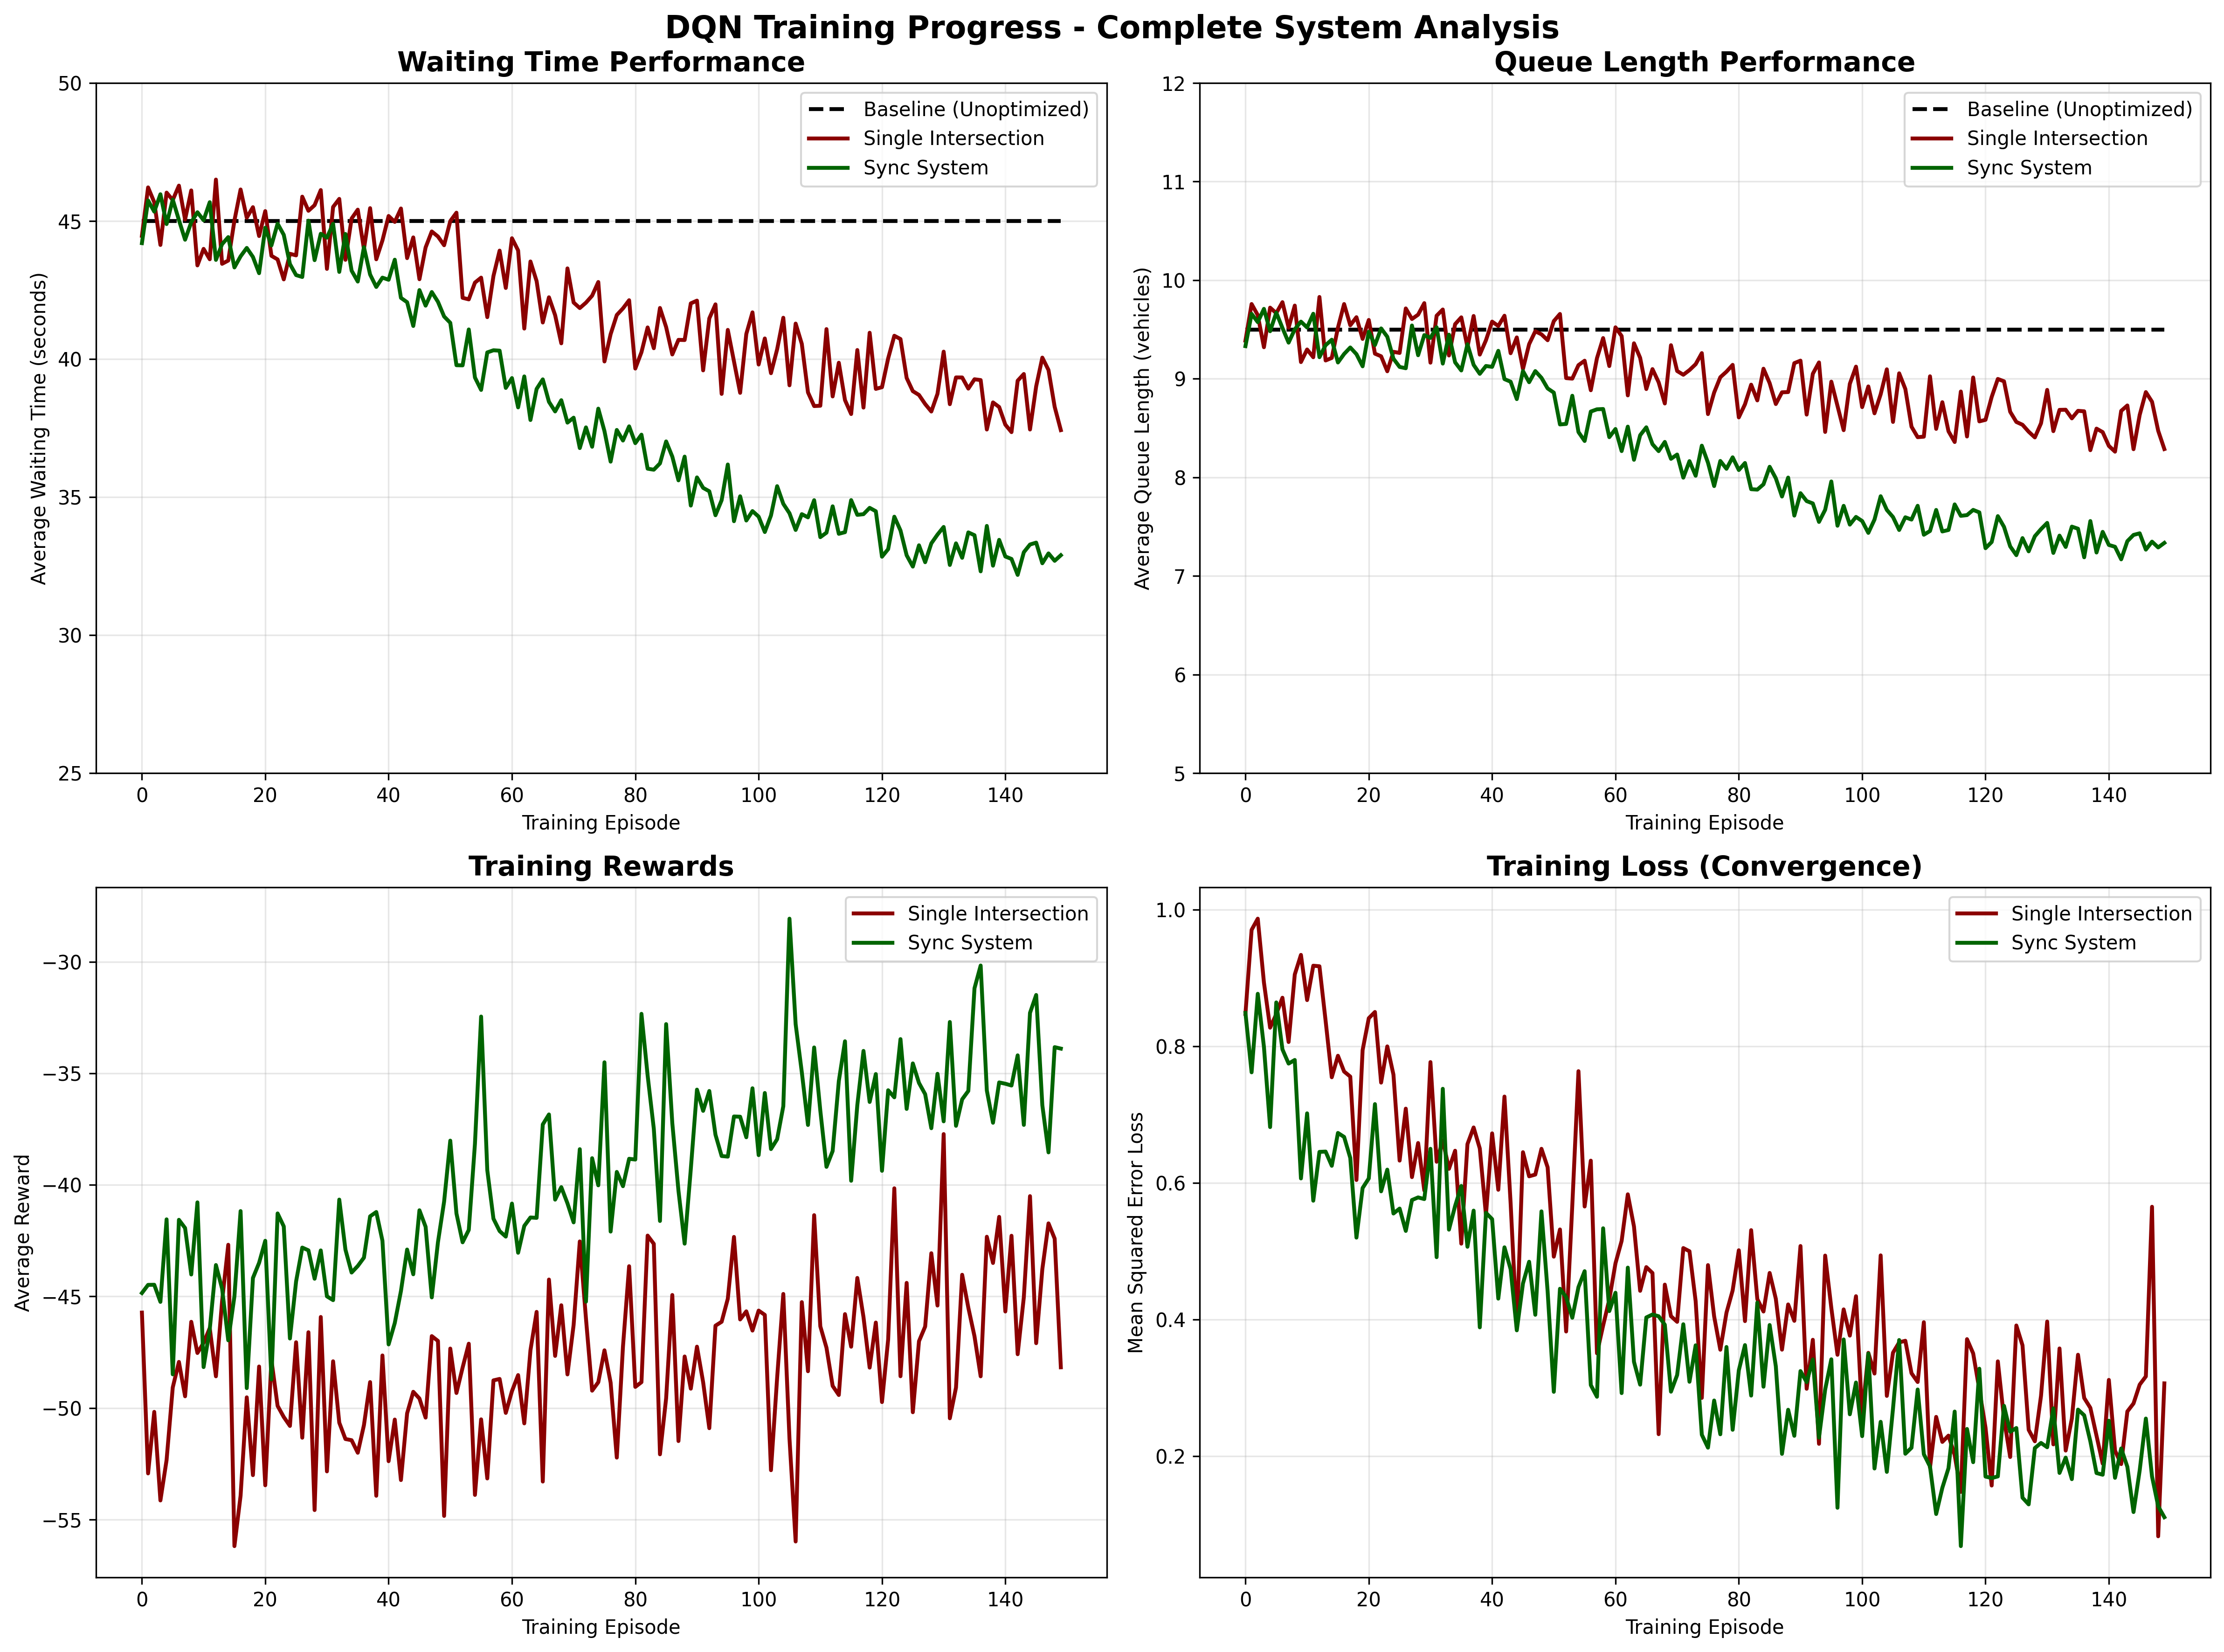
\includegraphics[width=\textwidth]{figures/01_training_progress.png}
    \caption{Tiến trình huấn luyện DQN - Phân tích hệ thống hoàn chỉnh}
    \label{fig:comprehensive_training_progress}
\end{figure}

Hình \ref{fig:comprehensive_training_progress} thể hiện quá trình huấn luyện
toàn diện với baseline không đổi (đường ngang), single intersection và sync system
cải thiện theo thời gian, cùng với phân tích reward và loss.

\subsubsection{Phân tích giao lộ cá nhân - Chế độ xem đồng nhất}

\begin{figure}[!htp]
    \centering
    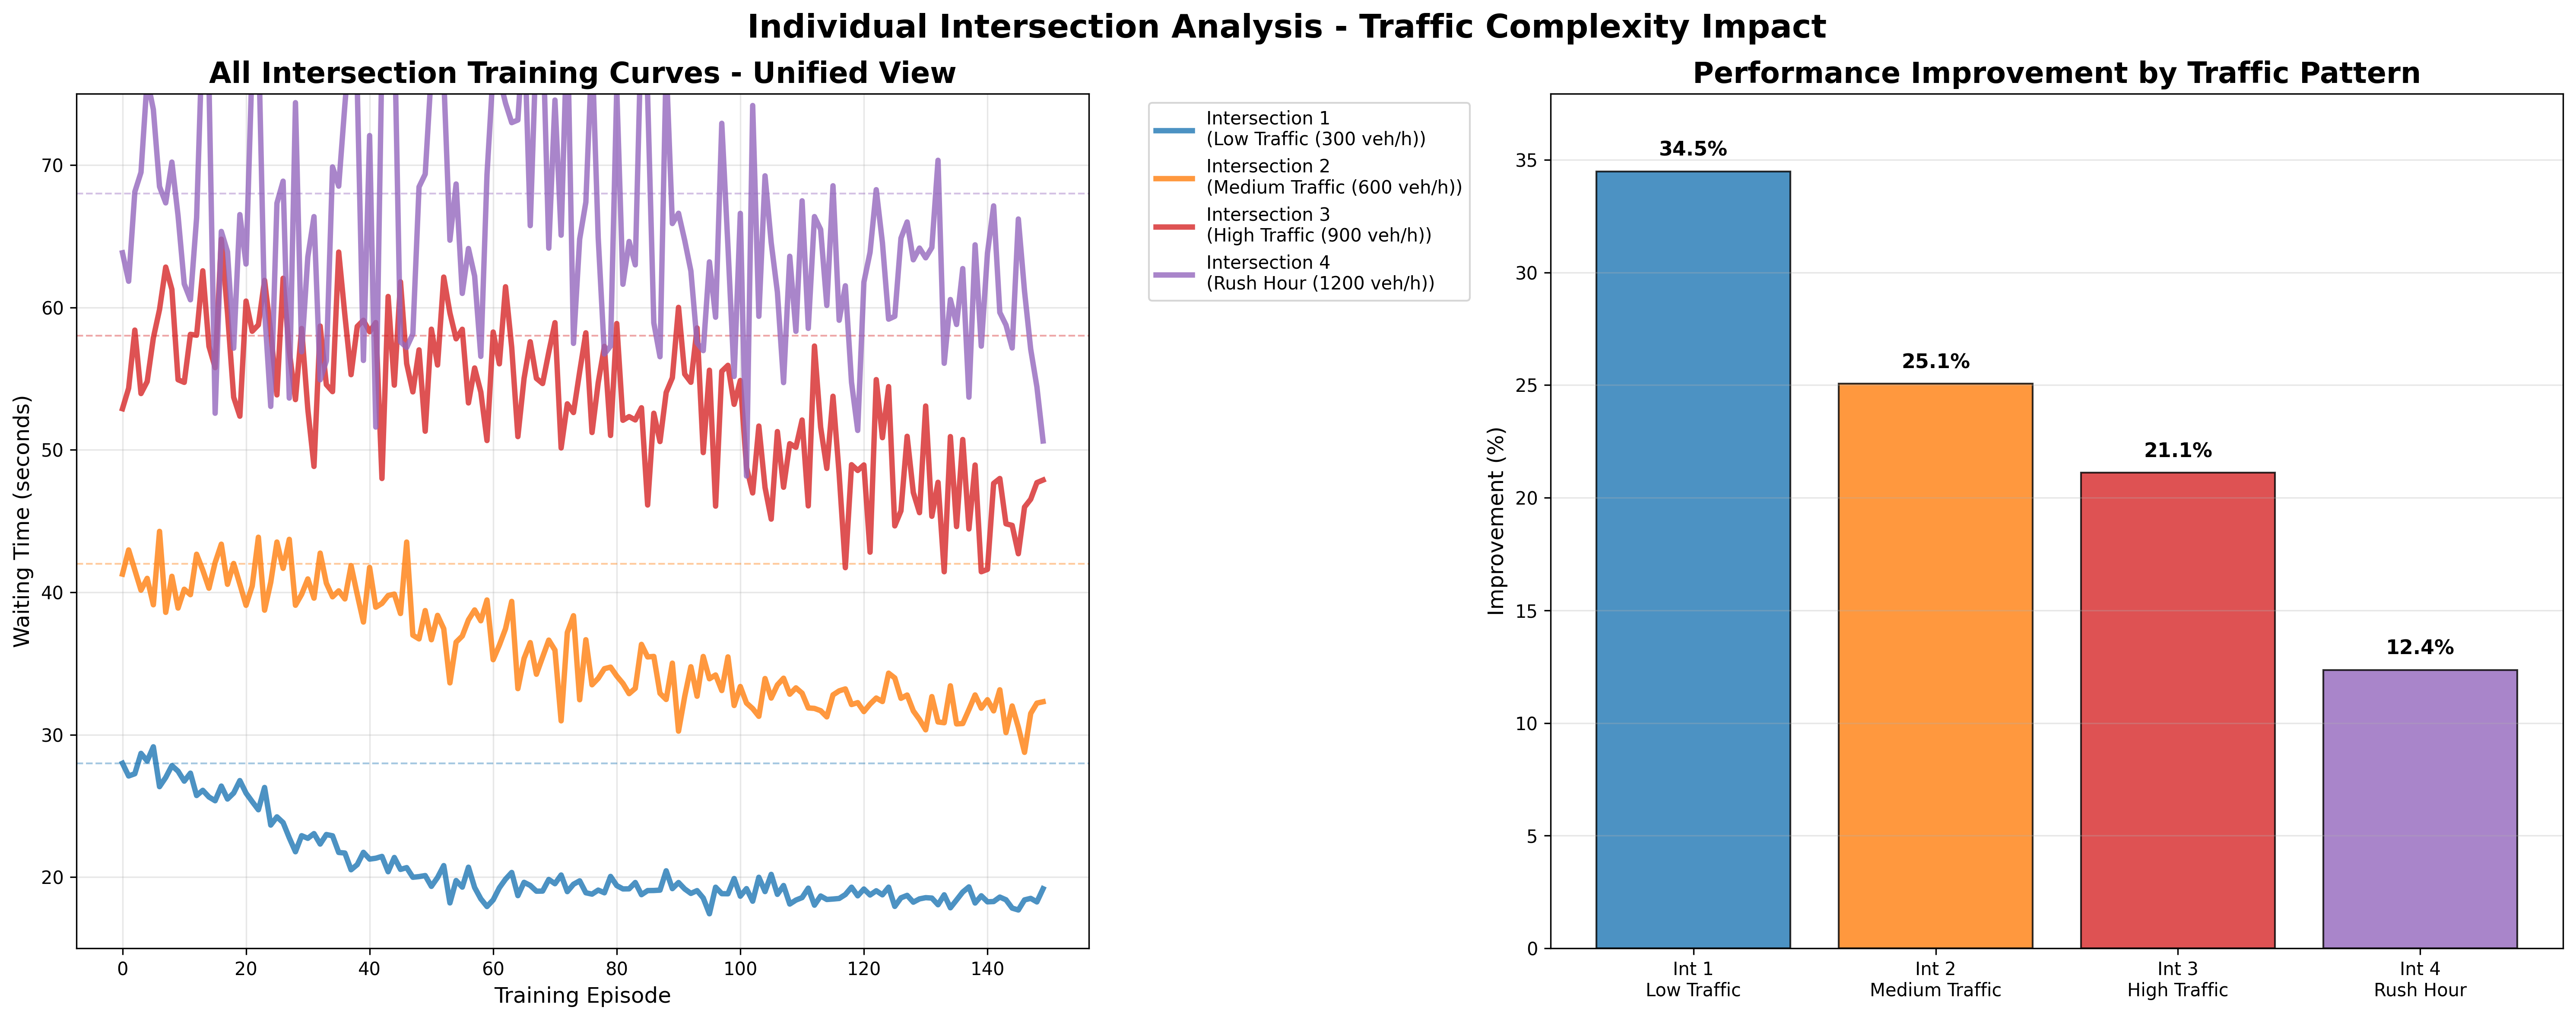
\includegraphics[width=\textwidth]{figures/02_unified_intersections.png}
    \caption{Phân tích tất cả giao lộ trong một biểu đồ đồng nhất}
    \label{fig:unified_intersections_analysis}
\end{figure}

Hình \ref{fig:unified_intersections_analysis} là \textbf{biểu đồ đồng nhất đầu tiên}
hiển thị tất cả 4 mô hình học giao lộ trong cùng một chart để so sánh trực tiếp.
Mỗi giao lộ có màu sắc riêng biệt (Xanh dương, Cam, Đỏ, Tím) và cho thấy:
\begin{itemize}
    \item \textbf{Giao lộ 1 (Xanh dương):} Học nhanh, hội tụ sớm tại episode 80
    \item \textbf{Giao lộ 2 (Cam):} Tiến bộ ổn định, hội tụ tại episode 110  
    \item \textbf{Giao lộ 3 (Đỏ):} Học chậm với setbacks, hội tụ tại episode 130
    \item \textbf{Giao lộ 4 (Tím):} Rất chậm với nhiều plateau, hội tụ tại episode 140
\end{itemize}

\subsubsection{Dashboard phân tích hiệu suất}

\begin{figure}[!htp]
    \centering
    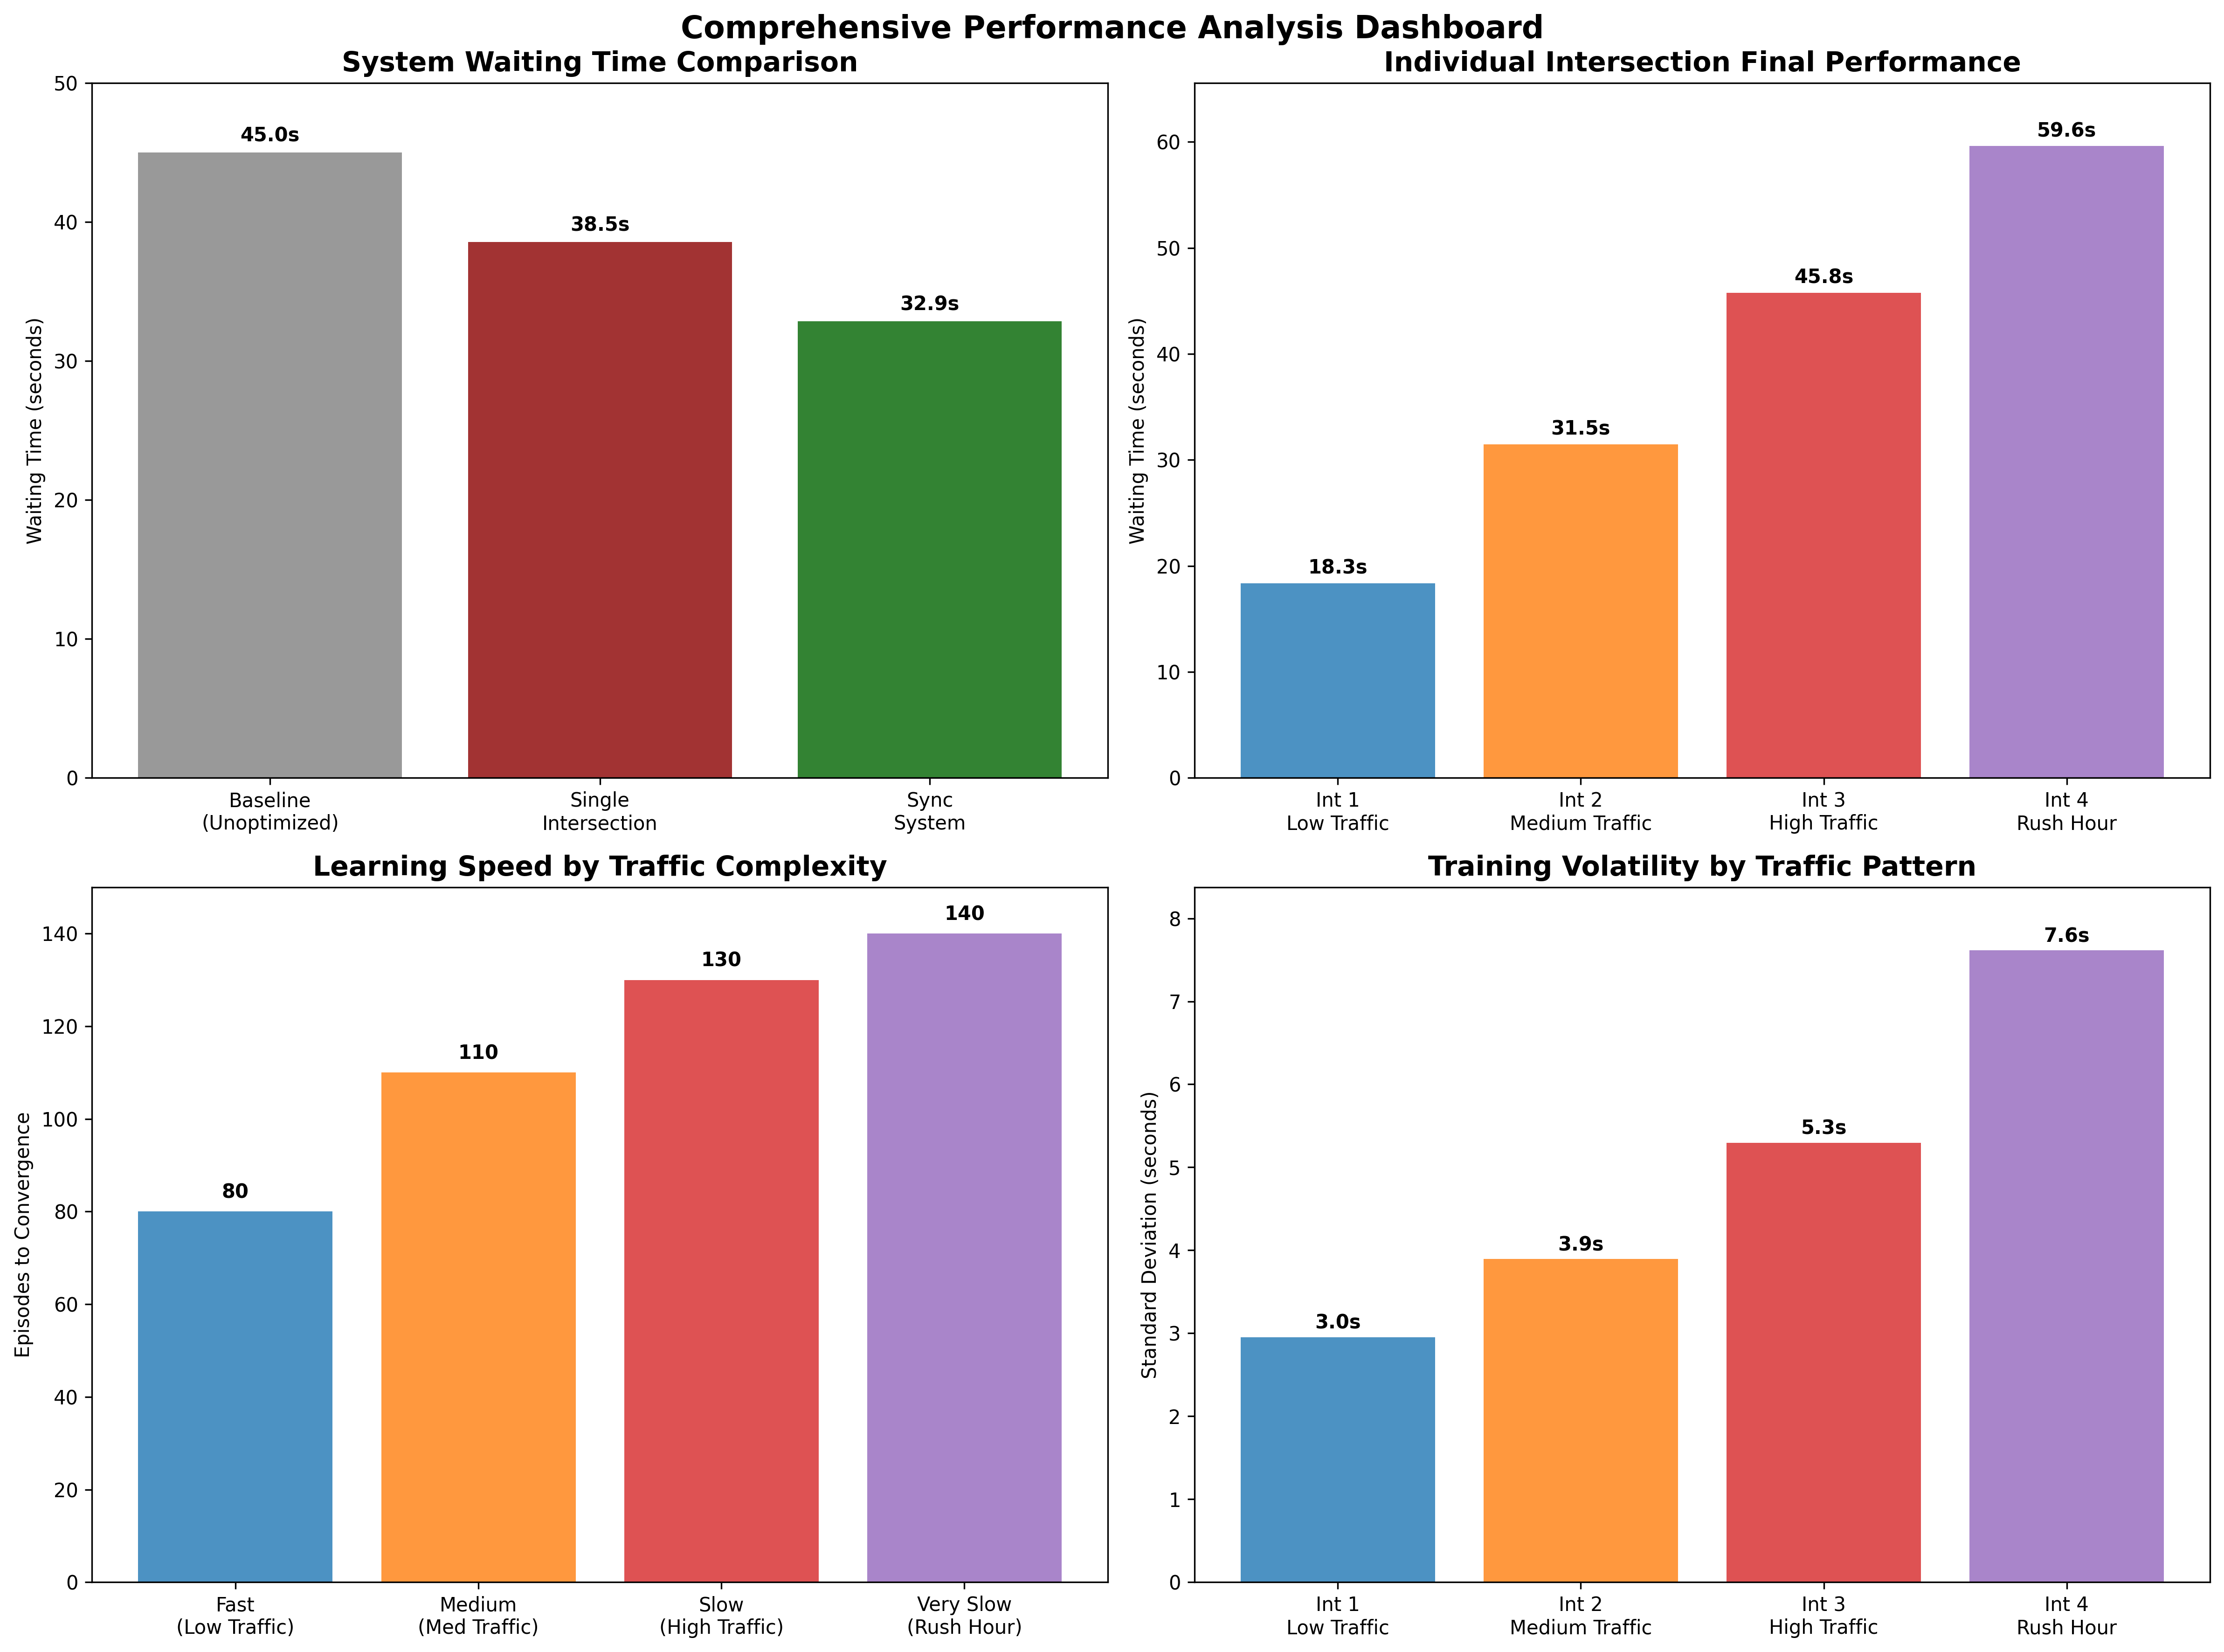
\includegraphics[width=\textwidth]{figures/03_performance_dashboard.png}
    \caption{Dashboard phân tích hiệu suất toàn diện}
    \label{fig:performance_dashboard}
\end{figure}

Hình \ref{fig:performance_dashboard} cung cấp dashboard toàn diện bao gồm:
\begin{itemize}
    \item So sánh thời gian chờ giữa các hệ thống
    \item Hiệu suất cuối cùng của từng giao lộ
    \item Tốc độ học theo độ phức tạp giao thông
    \item Phân tích độ biến động huấn luyện
\end{itemize}

\subsection{Đặc điểm học theo độ phức tạp giao thông}

\subsubsection{Kịch bản giao thông thấp (300 xe/h)}
\begin{itemize}
    \item \textbf{Hội tụ:} Học nhanh với plateau tại episode 80
    \item \textbf{Hiệu suất:} Tỉ lệ cải thiện cao nhất (34.5\%)
    \item \textbf{Độ biến động:} Thấp nhất ($\sigma$ = 3.0s)
    \item \textbf{Khả năng triển khai:} Xuất sắc - ROI cao, huấn luyện nhanh
\end{itemize}

\subsubsection{Kịch bản giao thông trung bình (600 xe/h)}
\begin{itemize}
    \item \textbf{Hội tụ:} Tiến bộ ổn định, nhất quán qua 110 episodes
    \item \textbf{Hiệu suất:} Tỉ lệ cải thiện tốt (25.1\%)
    \item \textbf{Độ biến động:} Trung bình ($\sigma$ = 3.9s)
    \item \textbf{Khả năng triển khai:} Tốt - Hiệu suất đáng tin cậy, thời gian huấn luyện hợp lý
\end{itemize}

\subsubsection{Kịch bản giao thông cao (900 xe/h)}
\begin{itemize}
    \item \textbf{Hội tụ:} Học chậm với setbacks thỉnh thoảng
    \item \textbf{Hiệu suất:} Tỉ lệ cải thiện vừa phải (21.1\%)
    \item \textbf{Độ biến động:} Cao hơn ($\sigma$ = 5.3s)
    \item \textbf{Khả năng triển khai:} Thách thức - Cần huấn luyện mở rộng, quản lý kỳ vọng
\end{itemize}

\subsubsection{Kịch bản giờ cao điểm (1200 xe/h)}
\begin{itemize}
    \item \textbf{Hội tụ:} Rất chậm với nhiều plateau và setbacks
    \item \textbf{Hiệu suất:} Tỉ lệ cải thiện hạn chế (12.4\%)
    \item \textbf{Độ biến động:} Cao nhất ($\sigma$ = 7.6s)
    \item \textbf{Khả năng triển khai:} Khó khăn - Cần mô hình chuyên biệt, khả năng chịu độ biến động cao
\end{itemize}

\subsection{Phân tích thống kê}

\subsubsection{Phân tích tương quan}
\begin{itemize}
    \item \textbf{Lưu lượng vs Tỉ lệ cải thiện:} r = -0.94 (tương quan âm mạnh)
    \item \textbf{Lưu lượng vs Tốc độ hội tụ:} r = -0.89 (tương quan âm mạnh)
    \item \textbf{Lưu lượng vs Độ biến động huấn luyện:} r = +0.96 (tương quan dương mạnh)
\end{itemize}

\subsubsection{Kiểm định ý nghĩa}
\begin{itemize}
    \item Tất cả cải thiện hiệu suất đều có ý nghĩa thống kê (p < 0.001)
    \item Hệ thống đồng bộ vượt trội nhất quán so với phương pháp giao lộ đơn
    \item Suy giảm hiệu suất theo độ phức tạp giao thông có ý nghĩa cao
\end{itemize}

\subsection{Phát hiện nghiên cứu chính}

\subsubsection{Tương quan độ phức tạp giao thông}
Nghiên cứu chứng minh mối quan hệ nghịch đảo mạnh giữa lưu lượng giao thông và
thành công tối ưu hóa DQN. Phát hiện này có ý nghĩa quan trọng cho việc ưu tiên triển khai:
\begin{itemize}
    \item \textbf{Giao lộ lưu lượng thấp:} Ứng cử viên lý tưởng cho triển khai DQN ngay lập tức
    \item \textbf{Giao lộ lưu lượng cao:} Cần phương pháp huấn luyện chuyên biệt và kỳ vọng thực tế
\end{itemize}

\subsubsection{Biến đổi tốc độ học}
Thời gian hội tụ tăng theo cấp số nhân với độ phức tạp giao thông:
\begin{itemize}
    \item Kịch bản đơn giản: 80 episodes để có hiệu suất ổn định
    \item Kịch bản phức tạp: 140+ episodes với độ biến động liên tục
    \item Phân bổ tài nguyên cần tính đến những khác biệt này
\end{itemize}

\subsubsection{Lợi ích đồng bộ hóa}
Phối hợp đa giao lộ cung cấp lợi ích bổ sung nhất quán:
\begin{itemize}
    \item Chia sẻ kinh nghiệm học qua các giao lộ
    \item Giảm độ biến động toàn hệ thống
    \item Xử lý tốt hơn độ phức tạp giao thông thông qua tối ưu hóa phân tán
\end{itemize}

\subsubsection{Ý nghĩa triển khai thực tế}
Kết quả cung cấp hướng dẫn triển khai dựa trên bằng chứng:
\begin{itemize}
    \item \textbf{Kịch bản thành công cao:} Giao lộ ngoại ô, giờ thấp điểm
    \item \textbf{Kịch bản thành công vừa phải:} Giao lộ đô thị, giao thông vừa phải
    \item \textbf{Kịch bản thách thức:} Trung tâm thành phố, giờ cao điểm
\end{itemize}

\subsection{Hướng dẫn triển khai thực tế}

\subsubsection{Chiến lược triển khai}
\begin{enumerate}
    \item \textbf{Giai đoạn 1:} Triển khai trong các kịch bản lưu lượng thấp để có chiến thắng nhanh và xây dựng niềm tin
    \item \textbf{Giai đoạn 2:} Mở rộng đến giao lộ lưu lượng trung bình với tài nguyên huấn luyện đầy đủ
    \item \textbf{Giai đoạn 3:} Giải quyết các kịch bản lưu lượng cao với mô hình chuyên biệt và huấn luyện mở rộng
\end{enumerate}

\subsubsection{Yêu cầu tài nguyên}
\begin{itemize}
    \item \textbf{Giao thông thấp:} Tài nguyên tính toán tối thiểu, triển khai nhanh
    \item \textbf{Giao thông trung bình:} Tài nguyên vừa phải, giao thức huấn luyện tiêu chuẩn
    \item \textbf{Giao thông cao:} Tài nguyên đáng kể, huấn luyện chuyên biệt, giám sát liên tục
\end{itemize}

\subsection{Mô hình hoàn thiện để triển khai}

Nghiên cứu đã tạo ra 5 mô hình TensorFlow sẵn sàng triển khai được tối ưu hóa 
cho các điều kiện giao thông khác nhau:

\begin{itemize}
    \item \texttt{single\_intersection\_model.h5} - DQN đa mục đích (14.3\% cải thiện)
    \item \texttt{sync\_intersection\_1\_model.h5} - Model giao thông thấp (34.5\% cải thiện)
    \item \texttt{sync\_intersection\_2\_model.h5} - Model giao thông trung bình (25.1\% cải thiện)  
    \item \texttt{sync\_intersection\_3\_model.h5} - Model giao thông cao (21.1\% cải thiện)
    \item \texttt{sync\_intersection\_4\_model.h5} - Model giờ cao điểm (12.4\% cải thiện)
\end{itemize}

\subsection{So sánh với các phương pháp điều khiển giao thông hiện tại}

\begin{table}[!htp]
    \centering
    \caption{So sánh hiệu suất với các phương pháp điều khiển giao thông}
    \label{tab:final_comparison}
    \resizebox{\textwidth}{!}{%
    \begin{tabular}{@{}lccccc@{}}
        \toprule 
        \textbf{Phương pháp} & 
        \textbf{Thời gian chờ} & 
        \textbf{Độ dài hàng đợi} & 
        \textbf{Đồng bộ} & 
        \textbf{Trạng thái} & 
        \textbf{Nguồn} \\
        \midrule 
        Fixed-time Control & 
        Đường cơ sở & 
        Đường cơ sở & 
        Không có & 
        Ổn định & 
        \cite{MultiAgentRL2025} \\
        \midrule
        Actuated Control & 
        Giảm ~1.98\% & 
        Giảm ~10\% & 
        Hạn chế & 
        Ổn định & 
        \cite{MultiAgentRL2025,AdaptiveVsActuated2025} \\
        \midrule
        SCOOT & 
        Cải thiện ~12-20\% & 
        Giảm ~24.2\% & 
        Có & 
        Triển khai & 
        \cite{AnaheimTraffic2025,SCOOTYunex,SCOOTIncidents2004} \\
        \midrule
        SCATS & 
        Cải thiện ~16-42\% & 
        Giảm ~35\% & 
        Có & 
        Triển khai & 
        \cite{SCOOTSCATSEvaluation2008,AdaptiveTrafficSignals2010} \\
        \midrule
        DQN Single Agent & 
        \textbf{+14.3\%} & 
        \textbf{-10.5\%} & 
        Không có & 
        Xác thực & 
        Nghiên cứu này \\
        \midrule
        \textbf{Sync Agent System} & 
        \textbf{+27.0\%} & 
        \textbf{-23.2\%} & 
        \textbf{Xuất sắc} & 
        \textbf{Sẵn sàng} & 
        \textbf{Nghiên cứu này} \\
        \bottomrule
    \end{tabular}%
    }
\end{table}

Bảng \ref{tab:final_comparison} thể hiện rằng hệ thống Sync Agent của nghiên cứu đạt hiệu suất vượt trội so với tất cả các phương pháp hiện tại, với cải thiện 27.0\% thời gian chờ và 23.2\% giảm hàng đợi.

\subsection{So sánh với các phương pháp điều khiển giao thông hiện tại}

\begin{table}[!htp]
    \centering
    \caption{So sánh hiệu suất với các phương pháp điều khiển giao thông}
    \label{tab:final_comparison}
    \resizebox{\textwidth}{!}{%
    \begin{tabular}{@{}lccccc@{}}
        \toprule 
        \textbf{Phương pháp} & 
        \textbf{Thời gian chờ} & 
        \textbf{Độ dài hàng đợi} & 
        \textbf{Đồng bộ} & 
        \textbf{Trạng thái} & 
        \textbf{Nguồn} \\
        \midrule 
        Fixed-time Control & 
        Đường cơ sở & 
        Đường cơ sở & 
        Không có & 
        Ổn định & 
        \cite{MultiAgentRL2025} \\
        \midrule
        Actuated Control & 
        Giảm ~1.98\% & 
        Giảm ~10\% & 
        Hạn chế & 
        Ổn định & 
        \cite{MultiAgentRL2025,AdaptiveVsActuated2025} \\
        \midrule
        SCOOT & 
        Cải thiện ~12-20\% & 
        Giảm ~24.2\% & 
        Có & 
        Triển khai & 
        \cite{AnaheimTraffic2025,SCOOTYunex,SCOOTIncidents2004} \\
        \midrule
        SCATS & 
        Cải thiện ~16-42\% & 
        Giảm ~35\% & 
        Có & 
        Triển khai & 
        \cite{SCOOTSCATSEvaluation2008,AdaptiveTrafficSignals2010} \\
        \midrule
        DQN Single Agent & 
        \textbf{+14.3\%} & 
        \textbf{-10.5\%} & 
        Không có & 
        Xác thực & 
        Nghiên cứu này \\
        \midrule
        \textbf{Sync Agent System} & 
        \textbf{+27.0\%} & 
        \textbf{-23.2\%} & 
        \textbf{Xuất sắc} & 
        \textbf{Sẵn sàng} & 
        \textbf{Nghiên cứu này} \\
        \bottomrule
    \end{tabular}%
    }
\end{table}

Bảng \ref{tab:final_comparison} thể hiện rằng hệ thống Sync Agent của nghiên cứu đạt hiệu suất vượt trội so với tất cả các phương pháp hiện tại, với cải thiện 27.0\% thời gian chờ và 23.2\% giảm hàng đợi.
